\documentclass[11pt,a4paper,twocolumn]{report}
\usepackage[margin=2cm]{geometry}

%-- Encoding, Language --%

\usepackage[utf8]{inputenc}
\usepackage[danish]{babel}

%-- Included Packages --%

\linespread{1.2}
\usepackage{eso-pic}
\usepackage{graphicx}
\usepackage{amsthm}
\usepackage{amsmath}
\usepackage{url}
\usepackage{tikz}
\usepackage{amsfonts}
\usepackage{lscape}
\usepackage{graphicx}
\usepackage[babel]{csquotes}
\usepackage{capt-of}
\usepackage{minted}
\usepackage[toc,page]{appendix}
\usepackage{caption}
\usepackage{hyperref}
\usepackage{listings}
\usepackage{color}

%-- Code listings --%
\definecolor{codegreen}{rgb}{0,0.6,0}
\definecolor{codegray}{rgb}{0.5,0.5,0.5}
\definecolor{codepurple}{rgb}{0.58,0,0.82}
\definecolor{backcolour}{rgb}{0.95,0.95,0.92}
\lstdefinestyle{codestyle}{
    backgroundcolor=\color{backcolour},   
    commentstyle=\color{codegreen},
    keywordstyle=\color{magenta},
    numberstyle=\tiny\color{codegray},
    stringstyle=\color{codepurple},
    basicstyle=\footnotesize,
    breakatwhitespace=false,         
    breaklines=true,                 
    captionpos=b,                    
    keepspaces=true,                 
    numbers=left,                    
    numbersep=5pt,                  
    showspaces=false,                
    showstringspaces=false,
    showtabs=false,                  
    tabsize=2
}
\lstset{style=codestyle}

%-- Bibliography --%

%\usepackage[backend=biber,style=verbose]{biblatex}
\usepackage[
    hyperref=auto,
    backend=bibtex,
    sorting=ynt,
    style=alphabetic, %numeric
    citestyle=alphabetic %verboze
]{biblatex}
\bibliography{bibliography}

%-- Authors --%

\author{
  Adam Honoré\\
  \texttt{030991-2721}\\
  \texttt{qgf142@alumni.ku.dk}
  \and
  Alexander Olsen\\
  \texttt{200692-2875}\\
  \texttt{bdj816@alumni.ku.dk}
  \and
  Rasmus Andersen\\
  \texttt{200491-2457}\\
  \texttt{hmd200@alumni.ku.dk}
}

%-- Title --%

\title{
  \vspace{3cm}
  \Huge{Bachelorprojekt} \\
  \Large{Fitts' lov}
}

%-- Frontpage, TOC --%
\begin{document}

\AddToShipoutPicture*{
    \put(0,0){
        \includegraphics*[viewport=0 0 700 600]{include/natbio-farve}}}
\AddToShipoutPicture*{
    \put(0,602){
        \includegraphics*[viewport=0 600 700 1600]{include/natbio-farve}}}
\AddToShipoutPicture*{
    \put(0,0){
        \includegraphics*{include/nat-en}}}

\clearpage\maketitle
\thispagestyle{empty}
\newpage
\tableofcontents
\newpage

%\begin{abstract}

%\end{abstract}

\addcontentsline{toc}{chapter}{Indledning}
\chapter*{Indledning}
I 1954 udgav Paul M. Fitts en artikel\footcite{fitts1954} som søgte at finde informationskapaciteten af det menneskelige motoriske system - og dermed en generel formulering for sammenhængen mellem distancen til og størrelsen af et mål i en motorisk opgave og den tid det tager at udføre opgaven. Fitts så et behov for et samlende begreb for den menneskelige motoriske kapacitet, grundet de tydelige problemer med at forene mange af de fakta, der var blevet beskrevet i tidligere litteratur. Hans forklaring var, at der var blevet overset en overordnet sammenhæng mellem amplituden, varigheden og variabiliteten i bevægelserne ved motoriske opgaver.


\addcontentsline{toc}{chapter}{Teori}
\chapter*{Teori}
%For at påvise den sammenhæng som Fitts mente var til stede, udførte han en række eksperimenter\footcite{fitts1954}, hvorfra han ud fra indsamlet data kunne opstille en formel til at beskrive den tid det tager at udføre en given motorisk opgave afhængigt af afstanden til og størrelsen på målet. I alt udførte Fitts tre eksperimenter, det første af dem dog med to forskellige pegeredskaber, hvilket gav anledning til data fra fire forskellige motoriske opgaver.
I dette kapitel vil vi kigge nærmere på teorierne bag Fitts' lov. Vi vil først give en opsumering af Fitts' egne tanker, hvorefter vi beskriver tre alternative formulering af Fitts' lov.

\addcontentsline{toc}{section}{Fitts' tre eksperimenter}
\section*{Fitts' tre eksperimenter}
Fitts var interesseret i at vise at informationsteori kunne bruges til at beskrive det menneskelige motoriske system og udførte derfor en række eksperimenter\cite{fitts1954}. Fitts' udførte i alt tre eksperimenter, det første af dem dog med to forskellige pegeredskaber, hvilket gav anledning til data fra fire forskellige motoriske opgaver. Fitts' arbejdede med de tre eksperimenter udfra følgende hypotese, hvor $E$ er .... og $S$ er forsøgspersonen
\begin{quotation}
\textit{If the amplitude and tolerance limits of a task are controlled by E, and S is instructed to work at his maximum rate, then the average time per response will be directly proportional to the minimum average amount of information per response demanded by the particular conditions of amplitude and tolerance.}
\end{quotation}
Vi vil i denne sektion se nærmere på de tre eksperimenter og Fitts konklusioner.

\addcontentsline{toc}{subsection}{Eksperiment 1}
\subsection*{Eksperiment 1: \textit{Reciprocal Tapping}}
Fitts gjorde i dette eksperiment brug af et pegeredskab og seks plader af samme længde. De to af pladerne, centerpladerne, var placeret med en forudbestemt afstand imellem sig, imens én af hver af de sidste fire plader blev placeret på hver side af centerpladerne. De to centerplader kunne antage fire forskellige bredder og de kunne placeres på fire måder, hver med en ny afstand imellem dem. Testpersonen skulle gentagene gange føre pegeredskabet fra den ene centerplade til den anden med vægt på præcision frem for fart, de omkringliggende pladers formål var at måle eventuelle fejl. Figur \ref{fig:FittsEx1} viser opstillingen, hvor de to stiplede plader er centerpladerne.

Testdeltagerne, 16 højrehåndede universitetsstuderende mænd, fik 15 sekunder til hver af de 16 opgaver i tilfældig rækkefølge med en mellemliggende pause på 55 sekunder imellem hver af dem. Eksperimentet blev udført med to forskellige pegeredskaber et lettere i vægt end det andet.

\begin{figure}[h]
\centering
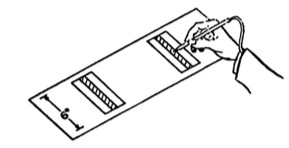
\includegraphics{images/illustrations/fitt_ex1}
\caption{Opstillingen brugt til Fitts' første eksperiment \footcite{fitts1954}}
  \label{fig:FittsEx1}
\end{figure}

\addcontentsline{toc}{subsection}{Eksperiment 2}
\subsection*{Eksperiment 2: \textit{Disc Transfer}}
I dette eksperiment brugte Fitts to pinde og otte runde plader. De otte runde plader havde et hul i midten som kunne antage fire forskellige størrelser, dog havde alle otte plader den samme hulstørrelse i hver enkel opgave. De to pinde kunne ligesom i eksperiment 1 være placeret med fire forskellige afstande imellem sig. 

Hver af de 16 forsøgsmuligheder blev i tilfældig rækkefølge udført af 16 højrehåndede universitetsstuderende mænd. Figur \ref{fig:FittsEx2} viser, hvordan eksperimentet blev udført.
\begin{figure}[h]
\centering
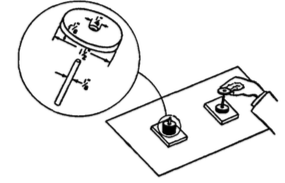
\includegraphics[scale=0.9]{images/illustrations/fitt_ex2}
\caption{Opstillingen brugt til Fitts' andet eksperiment \footcite{fitts1954}}
\label{fig:FittsEx2}
\end{figure}

\addcontentsline{toc}{subsection}{Eksperiment 3}
\subsection*{Eksperiment 3: \textit{Pin Transfer}}
Udførelsen af dette eksperiment krævede et sæt af otte pinde og 16 huller delt i to sæt. Diameteren på de otte pinde kunne antage fire forskellige størrelser alt imens afstanden imellem de to sæt huller kunne være af fem forksellige længder, opstillingen kan ses af figur \ref{fig:FittsEx3}.

Hver af de 20 mulige forsøgsopstillinger blev udført i tilfældig rækkefølge af 20 universitetsstuderende mænd.
\begin{figure}[h]
\centering
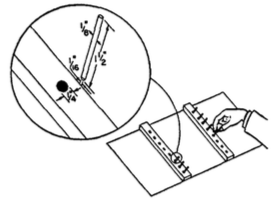
\includegraphics[scale=0.9]{images/illustrations/fitt_ex3}
\caption{Opstillingen brug til Fitts' tredje eksperiement \footcite{fitts1954}}
\label{fig:FittsEx3}
\end{figure}

\addcontentsline{toc}{subsection}{Fitts' konklusion}
\subsection*{Fitts' konklusion}
Resultaterne som Fitts fik fra de udførte eksperimenter viste, at des større afstand målene imellem desto længere tid brugte testdeltagerne. For at bevise sin teori udledte Fitts et \textit{Index of Difficulty}, ID, som beskriver sværhedsgraden af en given motorisk opgave på baggrund af størrelsen, $W$, på og afstanden, $A$, til målet.
\begin{align*}
ID = -\log_2\left(\frac{W}{2A}\right)
\end{align*}

Brugen af $\log_2$ i formlen er baseret på baggrund af Fitts kendskab til Shannon's sætning 17 \footcite{goldberg2015}. For at sikre, at ID altid giver en positiv værdi valgte Fitts at gøre brug af $2A$ frem for $A$, da det kan garanteres at $2A > W$, hvilket sikre det samme fortegn på logaritmen i alle tilfælde. Da $log\left(\frac{W}{2A}\right)<0$, for $0<\frac{W}{2A}<1$, valgte Fitts at multiplicere det med $-1$, hvilket sikre at ID altid er positiv.

Ved brug af ID udregnede Fitts et \textit{Index of Performance}, IP, som beskriver hvor godt en opgave er udført i forhold til sværhedsgraden, ID, og tiden $t$.
\begin{align*}
IP &= \frac{ID}{t}\Leftrightarrow\\
IP &= \frac{-1}{t}\log_2\left(\frac{W}{2A}\right)
\end{align*}

Denne formel er dog ikke den klassiske formel for Fitts lov, men ved matematiske omregninger kan den findes. Vi ser først på ID.
\begin{align*}
ID &= -\log_2\left(\frac{W}{2A}\right) \Leftrightarrow\\
ID &= -\log_2\left(W\right)-\left(-\log_2\left(2A\right)\right) \Leftrightarrow\\
ID &= \log_2\left(2A\right)-\log_2\left(W\right) \Leftrightarrow\\
ID &= log_2\left(\frac{2A}{W}\right)
\end{align*}
Vi kan indsætte dette i formlen for IP og isolere et udtryk for tiden $t$.
\begin{align*}
IP &=\frac{-1}{t}\log_2\left(\frac{W}{2A}\right) \Leftrightarrow\\ 
IP &= \frac{1}{t}\log_2\left(\frac{2A}{W}\right) \Leftrightarrow\\ 
t &= \frac{\log_2\left(\frac{2A}{W}\right)}{IP}
\end{align*}
Da det virker uoverskueligt i sådan en formel at dividere med IP så substitueres denne værdi med $IP = \frac{1}{b}$, hvilket giver en pænere formel.
\begin{align*}
t &= \frac{\log_2\left(\frac{2A}{W}\right)}{\frac{1}{b}} \Leftrightarrow\\ 
t &= b \cdot \log_2\left(\frac{2A}{W}\right)
\end{align*}
Når man regner med det menneskelige motoriske system, så skal der medregnes den tid det tager for et menneske at opfatte at en opgave er startet. Fitts fandt frem til denne faktor, $a$, ved at tilpasse sine data ved lineær regression.
\begin{equation}
\label{eq:FittsLov}
T = a + b \cdot log_2\left(\frac{2A}{W}\right)
\end{equation}
Dette er hvad der i dag kendes som Fitts lov.

\addcontentsline{toc}{section}{Alternative formuleringer}
\section*{Alternative formuleringer}
Siden udgivelsen af Fitts’ artikel, har flere forskere forsøgt at finde en formel, der passer bedre på det motoriske system, end Fitts’ originale lov. Der har indenfor menneske-datamaskine interaktion været flere udgivelser, som mener at have fundet en mere præcis formel end Fitts’ lov, eller som kigger på andre former for eksperimenter. Vi vil i dette afsnit se nærmere på tre sådanne formuleringer.

\addcontentsline{toc}{subsection}{Welfords formel}
\subsection*{Welfords formel}

I \cite{welford1968} beskriver Welford en række fundamentale forudsætninger for det menneskelige motoriske system. Her kiggede han blandt andet på Fitts' lov og de data han indsamlede i sit første forsøg. Han mente at Fitts' lov i princippet gengav den indsamlede data præcist, men han så også tre utilfredsstillende egenskaber, hvilket fik ham til at foreslå følgende modifikationer.
\begin{figure}[h]
\centering
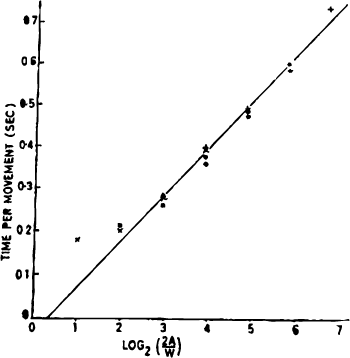
\includegraphics{images/illustrations/welford_plot}
\caption{Denne graf er pt medtaget for at kunne forklare Welford's tanker. Den vil blive erstattet af en pænere graf!}
\label{fig:WelfordGraf}
\end{figure}
Welford argumenteret for at der skulle undlades at multiplicere $A$ med $2$, da det på data fra Fitts' første forsøg ville resultere i en negativ $a$-værdi. Derved bliver Ligning \ref{eq:FittsLov} til
\begin{align}
\label{eq:Crossman}
T = a + b \cdot log\left(\frac{A}{W}\right)
\end{align}
som også tidligere var blevet udledt af Crossman\cite{crossman1957}. Hvis data fra Fitts' første forsøg indsættes i Ligning \ref{eq:Crossman}, så vil $a$ ligge tæt på $0.05$. Dette passer med Crossman's eksperiment, hvor han får tiden man bruger inden bevægelsen begynder til at være cirka $0.05$\cite{crossman1957}. Man kunne argumentere for at man derved helt kunne undlade $a$, da det beskriver tiden inden bevægelsen. I et lignende eksperiment\cite{welford1958} fandt man dog at resultaterne generelt var mere uniforme og plausible, hvis $a$-leddet var medtaget.

Den kurve der passer Figur \ref{fig:WelfordGraf} bedst ville være en let opdagående kurve. Welford mente at kurven kunne gøres væsentlig mindre, ved at lave følgende modifikationer til Ligning \ref{eq:FittsLov}:
\begin{align}\label{eq:WelfordsLov}
T = K \cdot log\left(\frac{A + \frac{1}{2}W}{W}\right) = K \cdot log\left(\frac{A}{W} + 0.5\right)
\end{align}
Ligning \ref{eq:WelfordsLov} er sidenhen blevet kendt som Welfords lov og har betydning for hvordan tiden, $T$, opfattes. Tiden vil i Ligning \ref{eq:WelfordsLov} blive afhænging af en Weber Fraction, da testpersonen skal skelne mellem længderne til målets fjerneste og næreste kant. Testpersonen skal altså udvælge en længde, $W$, ud fra den totale længde mellem startpunktet og målets fjerneste kant. Det er her vigtigt at notere at Ligning \ref{eq:WelfordsLov} også opretholder den fordel, som Fitts hævdede der var ved at multiplicere $A$ med $2$. Dette ses udfra det mest ekstreme tilfælde, hvor bevægelsens startpunkt er på målets kant, da $A = \frac{1}{2}W$ vil gælde, hvorved $T = K \cdot log\left(\frac{A + \frac{1}{2}W}{W}\right) = K \cdot log\left(\frac{W}{W}\right)$. Da $W > 0$ vil $log(W) > 0$.

Den sidste observation, der blev gjort, var at kurven i figur~\ref{fig:WelfordGraf} viser en tydelig udfladning i den lave ende. Welford noterede at det sandsynligvis var grundet en begrænsende faktor som beskriver en minimumstid per bevægelse, hvor kort eller uhindret bevægelse end måtte være. Welford's egne undersøgelser har påvist at denne begrænsende faktor har betydning for hvor meget af målet der rent faktisk bliver brugt. Når målene er brede og længden mellem dem kort, så vil testpersonen kun bruge en sub-længde af målets fulde længde. Han overfører mere information end Ligning \ref{eq:WelfordsLov} ville beskrive, fordi den effektive W er kortere. Den kortere bredde kan i nogen omfang afspejles i en reduktion af fejl og, hvis reduktionen sker med behørigt hensyn, så holder Ligning \ref{eq:WelfordsLov} stadig\footnote{Evt. skrive noget om hvordan fejl reduktionen sker: Welford FoS side 147-149}.

Ud fra de tre ovenstående modifikationer indførte Welford igen Fitts' data fra hans første forsøg i et koordinatsystem. Denne gang havde dataen dog været igennem fejl reduktion og blev indsat op imod Welford's formulering, hvilket viste at Ligning \ref{eq:WelfordsLov} var bedre til at beskrive dataen end Ligning \ref{eq:FittsLov} \footnote{Indsætte figur 5.4 fra FoS side 148}.

\addcontentsline{toc}{subsection}{MacKenzies formel}
\subsection*{MacKenzies formel}
MacKenzie udgav i 1992 en artikel~\cite{mackenzie1992}, hvor han ser nærmere på Fitts' Lov og seks alternative studier af samme. Han gennemgår en række forbedringer af den originale model, og fremstiller en alternativ formulering til $ID$, som han beskriver som værende mere teoretisk forsvarlig, nemlig:
\begin{align}
T=a+b\cdot\log_2\left({\frac{A+W}{W}}\right)
\end{align}

Han nævner i afsnittet \emph{Physical Interpretation} at skæringspunktet ideelt set vil ligge i nul, hvilket tyder på, at en opgave med $ID=0$ vil tage 0 sekunder. Ifølge MacKenzie modvises dette normalt ved lineær regression på forsøgsdata, som ofte medfører et skæringspunkt, der ikke ligger i nul. Dette bruger han som argument for, at der findes en additiv faktor som er urelateret til ID.\\

En af de mest accepterede udledninger af Fitts' lov stammer fra modellen \emph{deterministic error-corrections} originalt fremstillet af \cite{crossman1983}, og bygger på idéen om at en bevægelsesopgave består af en række iterative korrigerende bevægelser. MacKenzie refererer til simpliciteten af denne model som værende appellerende, men kalder de underliggende antagelser for suspekte. Han refererer til \cite{langolf1976}, hvor der blev observeret bevægelsesopgaver som kun indeholdte én korrigerende bevægelse, selvom det generelt forudses at der vil være flere korrigerende bevægelser ved en vis størrelse af $A/W$.\\

% TODO: Indsæt citat fra artiklen i stedet, for at give en idé om MacKencies holdning til Fitts' originale formulering
%MacKenzie ser Fitts' lov som en analogi med et behov for en teori til at støtte op om den - teori baseret på menneskelig motorik, ikke informationsteori.\\\\

\begin{figure}[h]
\centering
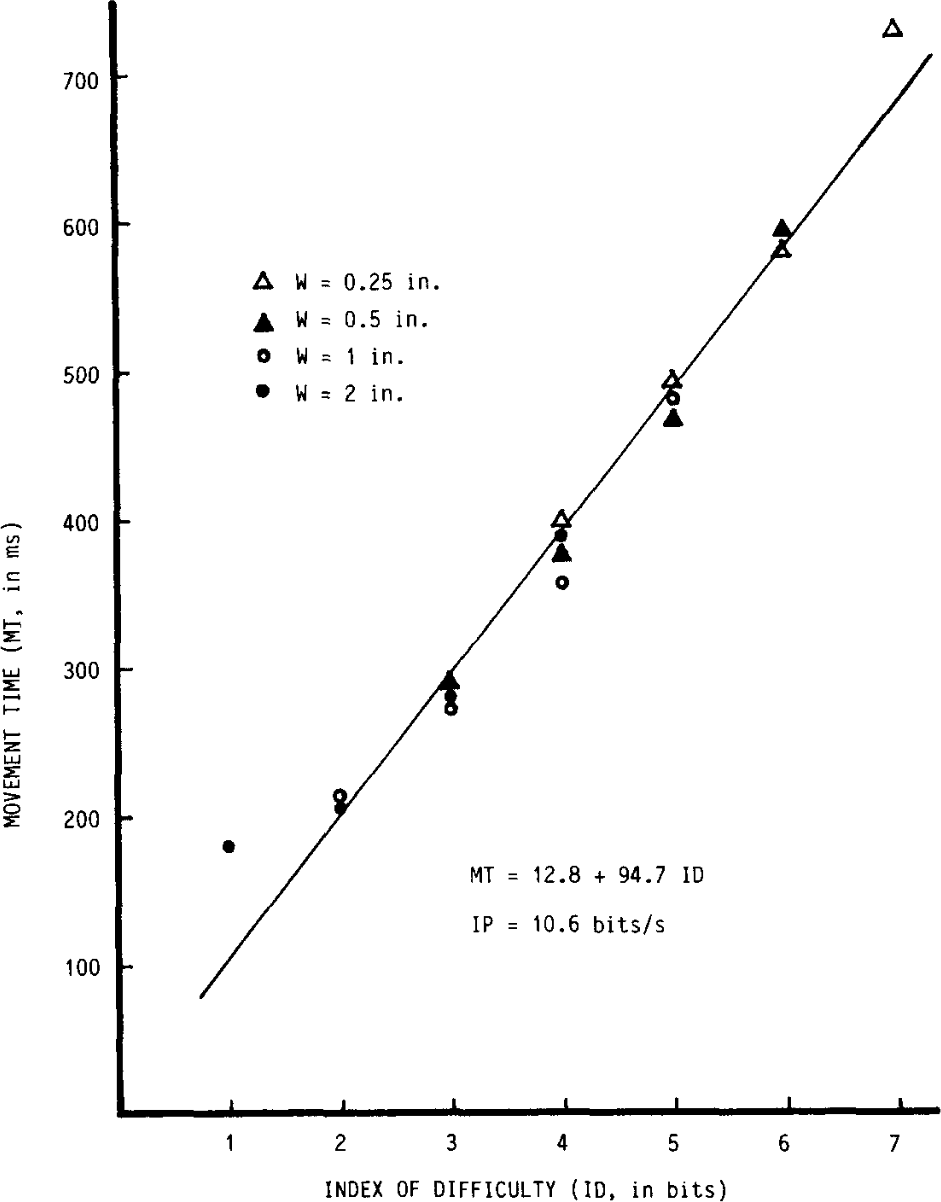
\includegraphics[scale=0.5]{images/illustrations/mackenzie_plot_1}
\caption{Index of difficulty i forhold til movement time ved forskellige værdier af $W$}
\label{fig:MacKenziePlot1}
\end{figure}
MacKenzie beskriver at et af problemerne med Fitts' Lov er den tætte relation mellem $ID$ og $MT$. Figur~\ref{fig:MacKenziePlot1} illustrerer hvordan punkterne flader ud, ved lave værdier af $ID$, mens kurven beholder sit $1:1$-forhold mellem $ID$ og $MT$. Der er altså en usammenhæng mellem de observerede og forudsagte værdier, hvilket også er blevet observeret i flere andre studier som \cite{welford1960, buck1986, crossman1983, drury1975, klapp1975, langolf1976, meyer1988, wallace1978}\\
Han fremhæver dog at der er lavet en del studier af Fitts' lov, og at der er blevet præsenteret en del alternative formuleringer som forsøger at få den reelle data til at passe bedre til modellen. Specielt fremhæver han Welford's~\cite{welford1960,welford1968}, da den er udbredt som alternativ til Fitts' originale formulering. MacKenzie nævner den ekstreme lighed mellem Welford og Shannons formulering, og beskriver hvordan det for nyligt er blevet vist at Paul Fitts originale formulerings forhold mellem $A$ og $W$ havde baggrund i en approksimation af Shannon's sætning~\cite[p. 388]{fitts1954}, som var blevet introduceret med en advarsel om at brugbarheden kun gjaldt ved et højt signal-til-støj forhold. Dette giver selvfølgelig problemer når der i Fitts' originale forsøg bliver brugt et forhold helt ned til 1:1 mellem A og W. MacKenzie foreslår at man benytter sig af en form der minder meget om Welford's, men her er en direkte analogi til Shannon's formulering:
\begin{align}
\text{Shannon: }C=B\times&\log{\frac{S+N}{N}}\\
\text{Welford: }MT=a+b\times&\log{\frac{A+0.5W}{W}}\\
\text{MacKenzie: }MT=a+b\times&\log{\frac{A+W}{W}}
\end{align}

Forskellen mellem Fitts' originale formulering for $ID$, og MacKenzie's bud på en ny formulering lavet som en direkte analogi til Shannon's bliver sammenlignet i figur~\ref{fig:MacKenziePlot2}, hvor det tydeligt at der ved lavere værdier af $A$ sker en udfladning af kurven, hvilket passer med data i figur~\ref{fig:MacKenziePlot1}.\\
\begin{figure}[h]
\centering
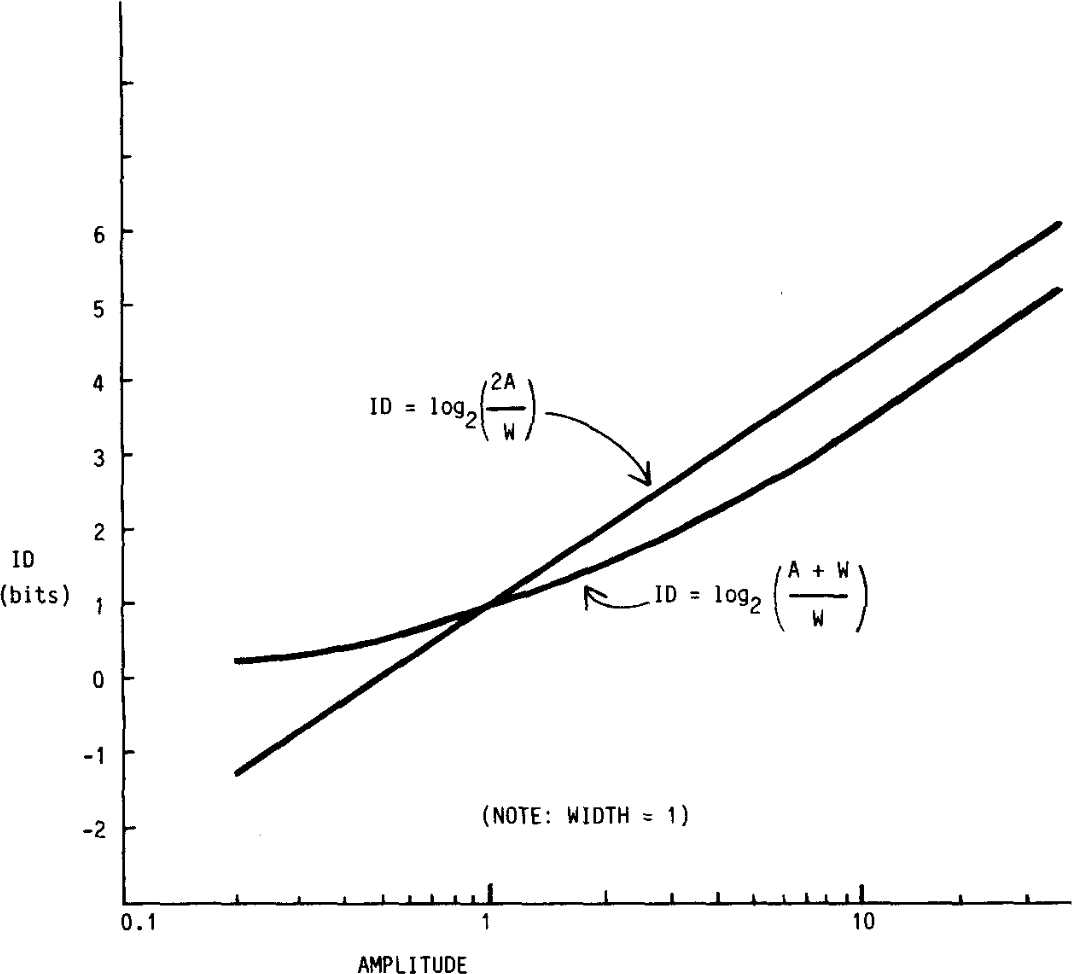
\includegraphics[scale=0.5]{images/illustrations/mackenzie_plot_2}
\caption{Sammenligning af Fitts' ID og MacKenzies ID baseret på Shannon's formulering}
\label{fig:MacKenziePlot2}
\end{figure}
MacKenzie ser hans formulering som værende en mindre forbedring i forhold til Welford's, og mener ikke at man vil kunne se den store forskel mellem Welfords og sin formulering, medmindre man har at gøre med $ID$ som er under 3 bits. Han kommer frem til de 3 bits ved at se på figur~\ref{fig:MacKenziePlot2} hvor det ses at de to formuleringer for $ID$ er paralelle med hinanden, indtil omkring 3 bits eller derunder.\\

Det generelle problem med MacKenzie's artikel er at han ikke kommer med noget teoretisk grundlag for hans formulering, og derved ikke kan forklare hvorfor hans formulering er mere præcis end andre, eller hvorfor det netop er bedre med en direkte analogi til Shannon's i forhold til Welford's. I artiklen~\cite{drewes2010} bliver der stillet spørgsmålstegn ved dette. Men hvis man ser bort fra det manglende teoretiske grundlag, så er MacKenzies formulering stadig en af de mest udbredte og brugte varianter af Fitt's lov, og har vist sig at passe godt på udførte forsøg~\cite{goldberg2015}.

\addcontentsline{toc}{subsection}{Meyers formel}
\subsection*{Meyers formel}
\begin{figure}[h]
\centering
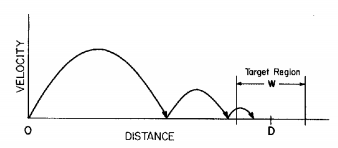
\includegraphics[scale=1.0]{images/illustrations/meyer_plot_theory}
\caption{Stochastic optimized-submovement modellen - Den horisontale akse repræsentere afstand og den vertikale akse bevægelseshastighed. De faste linjer repræsentere primære underbevægelser, mens stiplede linjer er korrigerende underbevægelser. Bevægelserne tager udgangspunkt i en startende position (afstand = 0) og skal bevæge sig til et mål, med center i D og bredde W.}
\label{fig:MeyerTheory}
\end{figure}
Som beskrevet i forrige afsnit, så basere Fitts' lov sig på \emph{deterministic error-corrections} modellen. Meyer et. al foreslog en ny model, kaldet stochastic optimized-submovement modellen, som de baserede deres formel på\cite{meyer1988}. Som det ses af Figur \ref{fig:MeyerTheory} så basere denne model sig på at personer laver en primær underbevægelse og derefter, hvis der er behov for det, en korrigerende underbevægelse. Udfra denne model kan den gennemsnitlige tid, $T$, forudsiges til at være
\begin{equation}
\label{eq:meyer}
T = a + b \sqrt{\frac{A}{W}}
\end{equation}

Meyer et. al udfører et teoretisk og to praktiske forsøg, hvor der i det teoretiske forsøg bliver gjort flere udregninger med forskellige værdier af A og W, som viser en god approksimation i forhold til Fitts' formulering. De praktiske forsøg gør brug af simplere motoriske opgaver end dem kendt fra Fitts' egne forsøg. Den eneste rummelige frihed i Meyers forsøg er håndledendes rotation. Derudover er det vigtigt at notere sig at Meyer igennem hele artiklen benytter sig af at en motorisk opgave er delt ind i en primær underbevægelse, og nogle efterfølgende korrigerende underbevægelser. Dette har dog ikke nogen betydning for sammenligningen med Fitts’ formulering, da den totale tid af alle underbevægelser vil approksimere den logaritmiske funktion af A/W, hvilket medfører at Fitts model også passer på modeller med iterative fejlkorrigerende underbevægelser.

Når man kigger på Ligning \ref{eq:meyer}, så er det vigtigt at notere sig, at den vil udvise en form svarende til $log_2(2A/W)$ og derved efterligne Ligning \ref{eq:FittsLov}. Grunden til dette er at $\sqrt{\frac{A}{W}}$ er en monotont voksende funktion, når $\frac{A}{W}$ bliver større. 

\cite{goldberg2015} notere dog at der er nogle ulemper ved denne formel. Hvis testdeltageren når målet i en enkelt bevægelse, så går modellen hen og bliver lineær, hvilket ikke passer godt med observeret værdier. For en fast positiv værdi af $\frac{A}{W}$ vil Meyers formel gå mod $1$, når antallet af underbevægelser går mod uendelig.

\addcontentsline{toc}{subsection}{Sammenligning}
\subsection*{Sammenligning}
Formlerne for de fire forskellige formuleringer af Fitts' lov, opridset i (9)-(12), 
\begin{align}
\text{Fitts: } T &= a+b\cdot\log\left(\frac{2A}{W}\right)\\
\text{Welford: } T &= K\cdot\log\left(\frac{A+0.5W}{W}\right)\\
\text{Mckenzie: } T &= a+b\cdot\log\left(\frac{A+W}{W}\right)\\
\text{Meyer: } T &= a+b\cdot\sqrt{\frac{A}{W}}
\end{align}

Welfords formulering har, indeholder den eneste, ikke nogen additiv konstant, $a$. Vi vil derfor omskrive (10) og forsøge at finde en formel som er lettere sammenligning med resten af formuleringerne.
\begin{align*}
T &= K\cdot\log\left(\frac{A+0.5W}{W}\right)\Leftrightarrow\\
T &= K\left(1-1+\log\left(\frac{A+0.5W}{W}\right)\right)\Leftrightarrow\\
T &= -K+K\left(1+\log\left(\frac{A+0.5W}{W}\right)\right)\Leftrightarrow\\
T &= -K+K\left(\log(2)+\log\left(\frac{A+0.5W}{W}\right)\right)\Leftrightarrow\\
T &= -K+K\left(\log\left(2\left(\cdot\frac{A+0.5W}{W}\right)\right)\right)\Leftrightarrow\\
T &= -K+K\cdot\log\left(\frac{2A+W}{W}\right)
\end{align*}

Bemærk, at dette resultat indeholder et negativt konstant led, $a=-K$. Dette ville betyde at tiden det tager for en testdeltager at påbegynde en opgave er negativ, og vi vil derfor kun benytte ID ledet af denne formel til den følgende sammenligning og ellers forkaste omskrivningen igen.

\begin{align*}
&\log\left(\frac{2A}{W}\right) &&\log\left(\frac{2A+W}{W}\right) &&&\log\left(\frac{A+W}{W}\right) &&&&\Leftrightarrow\\
&\log\left(2A\right) &&\log\left(2A+W\right) &&&\log\left(A+W\right) &&&&\Leftrightarrow\\
&1+\log(A) && 1+\log(A+0.5W) &&& &&&&\Leftrightarrow
\end{align*}

%\addcontentsline{toc}{section}{Forudsætninger for formuleringerne (Fitts vs Meyers vs Shannons)}

%\section*{Forudsætninger for formuleringerne (Fitts vs Meyers vs Shannons)}
%Sammenligning af en og to dimensioner

\newpage
\addcontentsline{toc}{chapter}{Design}
\chapter*{Design}
I dette afsnit beskriver vi det design der er brugt i vores forsøg. Derudover vil vi også beskrive vores forsøgsopstillinger.

\addcontentsline{toc}{section}{Forsøgsopstilling}
\section*{Forsøgsopstilling}
Vi har valgt at udføre to brugerundersøgelser, for at undersøge deltagernes bevægelsesbaner. Det første vil være et kontrolleret 'laboratorieeksperiment', mens det andet er et ukontrolleret crowdsourcing og webbaseret eksperiment.\\\\
Større dele af vores eksperiment har vi valgt at udføre ligesom tidligere udførte forsøg, da de er udført at folk med meget mere erfaring, og ekspertise på dette område, end os.
Det drejer sig om følgende dele af vores eksperiment:
\begin{itemize}
\item Spørgsmål som blev stillet før crowdsourcing-deltagerne kunne udføre forsøget\cite{goldberg2015}
\item Design af pegeopgave, inklusiv værdier af A og W\cite{goldberg2015}
\item Størrelser af A og W til tunnelopgave\cite{accot1997}
\item Antal vindinger af spiral til spiralopgave\cite{accot1997}
\end{itemize}
Derudover har vi brugt samme udformning af tunnel- og spiralopgave, som i pegeopgaven. Det vil sige, at vi har samme farver til mål, og samme design af testfladen.

\addcontentsline{toc}{section}{Platform og udviklingsværktøj}
\section*{Platform og udviklingsværktøj}
Vi har valgt at bruge JavaScript til at udvikle vores forsøg, da vi alle er bekendte med sproget, så vi skal ikke til at sætte os ind i noget nyt. Derudover er det integreret i alle browsere nu om dage, hvilket gør det nemt at crowdsource. For at generere vores opgaver har vi valgt at gøre brug af JavaScript-frameworket $paper.js$. Det gør brug af HTML5 canvas og er bagudkompatibelt til IE9. Frameworket gør det muligt at autogenerere cirkler til vores pegeopgaver, gemme bevægelsesbaner og tegne tunneller, til tunnelopgaverne.

\addcontentsline{toc}{section}{Opgavetyper}
\section*{Opgavetyper}
I denne sektion vil vi beskrive hvordan tunnel- og pegeopgaverne er designet.
 % Beskriv typen af opgaver ud fra ovenstående, antallet af opgaver, og hvor lang tid de skal vare

\addcontentsline{toc}{subsection}{Tunnelopgave}
\subsection*{Tunnelopgave}
I denne opgave skal testdeltageren føre markøren gennem fire tunneller af varierende længde og indmunding. Et eksempel på en sådan tunnel kan ses i Figur \ref{fig:tunnelopgaver}. Tunnellernes længde varierer med ($A = 100, 250, 300, 400$) og indmundingen med ($W = 20, 30 ,40, 50$), alle målt i pixel. Udmundingen vil i alle tilfælde være 8 pixels bred.

Ved begyndelsen af en opgave er to vertikale grønne linjer vist i hver ende af tunnellen. Når deltageren passerer første linje, fra venstre mod højre, vil linjen blive rød for at indikere at opgaven er i gang. Herefter vil en blå linje blive tegnet, hvor deltageren bevæger sin pegeenhed. Først når deltageren passerer anden linje fra venstre vil opgaven slutte, indikeret ved at de to vertikale linjer og bevægelsesbanen bliver gule. Næste opgave blev først startet når deltageren klikker på knappen 'continue', som kun er tilgængelig når én opgave er slut. I tilfælde af at testdeltageren rammer eller ryger uden for kanterne vil de kunne fortsætte ubemærket. Hele bevægelsesbanen og tiden det tager at gennemføre hver tunnel vil blive gemt.\\

\addcontentsline{toc}{subsection}{Spiralopgave}
\subsection*{Spiralopgave}
I denne opgave skal testdeltageren føre markøren gennem fire spiraler af varierende vindinger. Et eksempel på en sådan spiral kan ses i Figur \ref{fig:spiralopgave}. Spiralernes vindinger varierer med ($A = 1, 2, 3, 4$). Bredden er på de tre første spiraler ens, mens den sidste spiral kun har halv bredde af de tre forrige.

Ved begyndelsen af en opgave er spiralens udmunding markeret som en grøn streg. Når deltageren passerer denne linje, vil linjen blive stort. På samme tid vil den inderste linje i spiralen blive grøn. En grøn streg vil blive tegnet, hvor deltageren bevæger sin pegeenhed. Først når deltageren passerer den inderste linje vil opgaven slutte, indikeret ved at spiralen fjernes. Næste opgave blev først startet når deltageren klikker på knappen 'continue', som kun er tilgængelig når én opgave er slut. I tilfælde af at testdeltageren rammer eller ryger uden for kanterne vil de kunne fortsætte ubemærket. Hele bevægelsesbanen og tiden det tager at gennemføre hver tunnel vil blive gemt.
I denne opgave vil testdeltageren skulle føre markøren igennem fire spiraler af varierende størrelser og brede. Et eksempel på én af spiralerne kan ses i figur \ref{fig:spiralopgave}. Spiralerne kom i fire størrelser Hver test starter når testdeltageren fører musen forbi den grønne linje i spiralens indmunding

\addcontentsline{toc}{subsection}{Pegeopgave}
\subsection*{Pegeopgave}
I denne opgave vil testdeltageren blive præsenteret for en sekvens af 25 cirkulære mål af skiftene størrelse og position. Målene præsenteres i rækkefølgen som ses i Tabel \ref{tab:pegeopgave}. Hver test i sættet starter, når testdeltageren klikker inden for en fastplaceret cirkel i vinduets center og slutter når testdeltageren klikker indenfor målet. Hvert cirkulært mål varierer i distance fra center-cirklen og varierer i diameter, hvilket giver ændringer i A/W-sværhedsgrad som ses i Tabel \ref{tab:pegeopgave}. Center-cirklen vil  blive præsenteret i en grøn farve og vil ved klik skifte til blå - alle mål-cirklerne er vist i grøn farve. Et eksempel herpå ses i Figur \ref{fig:pegeopgave}. Vi vil i løbet af opgaven registrere tiden det tager fra at testpersonen trykker på center-cirklen, til de trykker på målet. Dertil vil banen som testdeltageren bruger også blive registreret.

\addcontentsline{toc}{subsection}{Generelt for de tre opgaver}
\subsection*{Generelt for de tre opgaver}
I alle opgaverne vil deltagerne blive informeret om, hvor mange opgaver de mangler at gennemføre, så de har en fornemmelse af, hvornår de er færdige. Hvis deltagerne bevæger pegeenheden uden for det canvas som opgaven skal udføres i vil denne del af banen ikke komme med i vores gemte data.

\addcontentsline{toc}{chapter}{Eksperimenter}
\chapter*{Eksperimenter}

\addcontentsline{toc}{section}{Udførsel af eksperimenter}
\section*{Udførsel af eksperimenter}

\addcontentsline{toc}{subsection}{Laboratorieeksperiment}
\subsection*{Laboratorieeksperiment}
Laboratorieeksperimentet vil blive udført af 10 tilfældigt udvalgte universitetsstuderende - dog ikke dataloger.
Forsøget foretages fra kl 9-13 - tidligt på dagen - for at sikre, at folk stadig er friske. Det vil foregå i en 4-personers sofabås på H.C. Ørstedsinstituttet, hvor der er privat og uden forstyrrelser.
Tidsmæssigt vil der være afsat 20 minutter til hver deltager, dog med plads til ekstra tid hvis nødvendigt.
Hver deltager bliver først introduceret til vores projekt og derefter introduceret til hhv. tunnel-, spiral- og pegeopgaven.
Herefter bliver testdeltageren bedt om at udføre tunnelopgaven - efterfulgt af spiral- og pegeopgaven - hvor der vil være et antal opgaver som skal udføres, hhv. 4 for tunnelopgaven, 4 for spiralopgaven og 25 for pegeopgaven.

\addcontentsline{toc}{subsection}{Crowdsourcingeksperiment}
\subsection*{Crowdsourcingeksperiment}
Crowdsourcingeksperimentet vil foregå på internettet, og vi har derfor gjort vores program tilgængeligt online. Ved crowdsourcingeksperimentet vil hver deltager udfylde formularen, som ses i Figur \ref{fig:Questions}, før de kan fortsætte. Når formularen er udfyldt forsætter deltageren til opgaverne. Her skal der, ligesom laboratorieeksperimentet, udføres 4 spiralopgaver, efterfulgt af 4 tunnelopgaver og til sidst 25 pegeopgaver. Efter deltageren har udført alle opgaver vil deres data blive sendt til en server, hvorefter deltageren får en informationsmeddelelse.
Vi har valgt at dele vores eksperiment på et antal af reddit-sider, da det er et meget populært internetfora, og muliggør at vi kan nå ud til så mange mennesker som overhovedet muligt.
\begin{itemize}
\item reddit.com/r/denmark\\
Vi valgte $/r/denmark$ fordi det er et aktivt subreddit.
\item reddit.com/r/helpme\\
\item reddit.com/r/care\\
Vi valte $/r/helpme$ og $/r/care$, da begge disse subredits er lavet til at spørge folk om hjælp.
\end{itemize}

Som det sidste vil vi også dele forsøget på vores egne Facebook-profiler.
\begin{figure}[h]
\centering
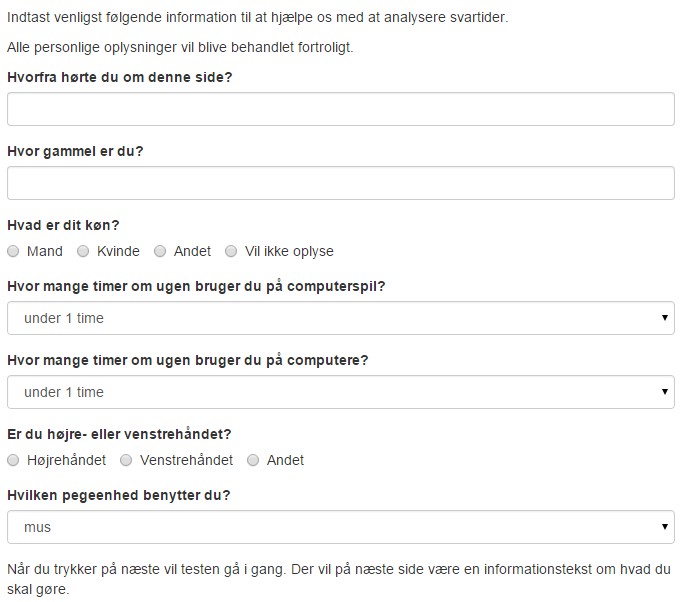
\includegraphics[scale=0.7]{images/screenshots/ex_questions}
\caption{Spørgsmål som blev stillet før crowdsourcing-deltagerne kunne udføre forsøget.}
\label{fig:Questions}
\end{figure}

\addcontentsline{toc}{section}{Resultat af eksperimenter}
\section*{Resultat af eksperimenter}

\addcontentsline{toc}{subsection}{Laboratorieeksperiment}
\subsection*{Laboratorieeksperiment}
Vi, P1, P2 og P3, udførte vores laboratorieeksperiment den 20. april 2015 på H.C. Ørsted instituttet. På trods af, at der på dagen ikke var mange mennesker til stede, så fik vi alligevel 10 personer igennem vores eksperiment i løbet af fire timer. De 10 testdeltagere var af varierende køn og nationalitet. Alle testdeltagere blev hvervet af P1 og blev derefter introduceret til eksperimentet af enten P2 eller P3. Herefter udførte alle testdeltagere forsøget uden behov for yderlig assistance. Testdeltagerne syntes godt om forsøget. Alt i alt forløb vores forsøg som forventet, uden problemer eller forstyrrelser.

\addcontentsline{toc}{subsection}{Crowdsourcingeksperiment}
\subsection*{Crowdsourcingeksperiment}
Forsøget gik godt - 264 personer gennemførte vores forsøg og har suppleret os med vital data. Vi fik delt vores forsøg på størstedelen af de tidligere beskrevne sider, dog med nogle få undtagelser. Generelt set var reddit det mest lukrative sted, hvorfra 140 personer har skrevet siden på som deres reference - hvorimod 74 skrev at de var blevet refereret fra Facebook.\\
Det var ikke muligt at dele vores forsøg på $reddit.com/r/helpme$ og $reddit.com/r/care$, da vi ikke havde nok "karma" for at kunne lave et indlæg på disse sites.\\
Efterfølgende har vi lukket for muligheden for at deltage i vores forsøg den 30/04/2015, og skrevet en besked på forsøgssiden hvor vi takker folk for deres deltagelse.

\begin{minipage}[t]{.5\textwidth}
\centering
\vspace{0pt}
\captionof{figure}{Illustration af pegeopgave}
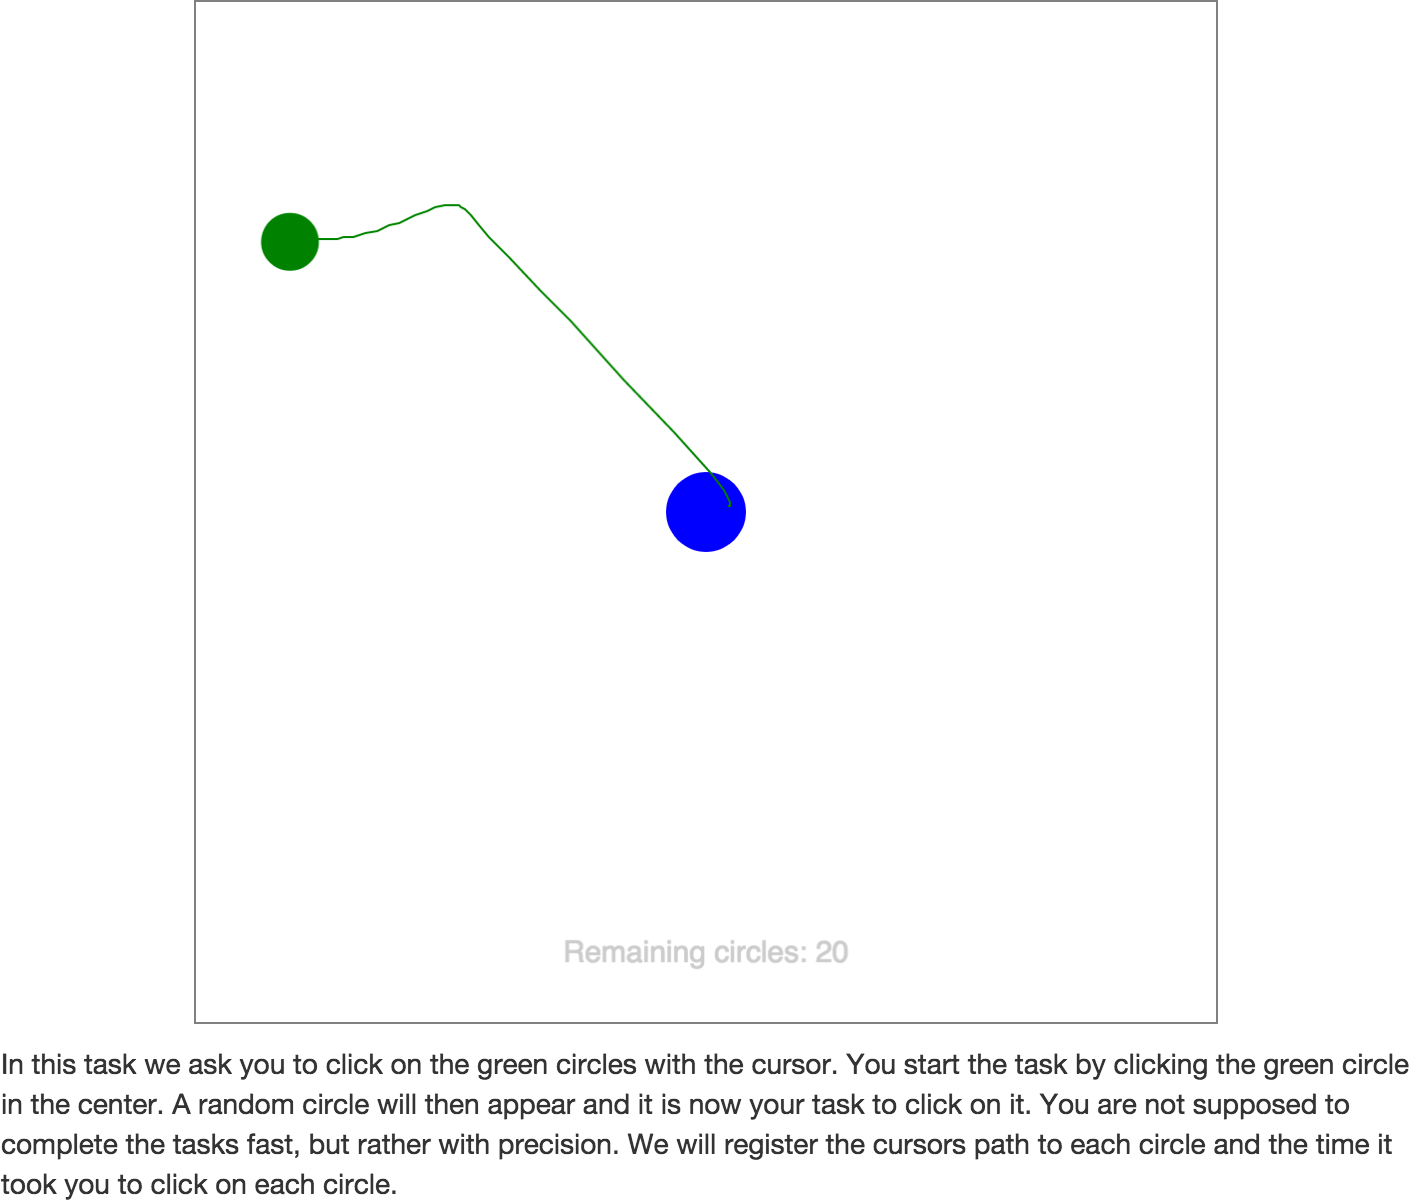
\includegraphics[width=\textwidth, trim = 7cm 20cm 15cm 5cm, clip]{images/screenshots/ex_step_6_pointing_path}
\label{fig:pegeopgave}
\caption{Illustration af tunnelopgave}
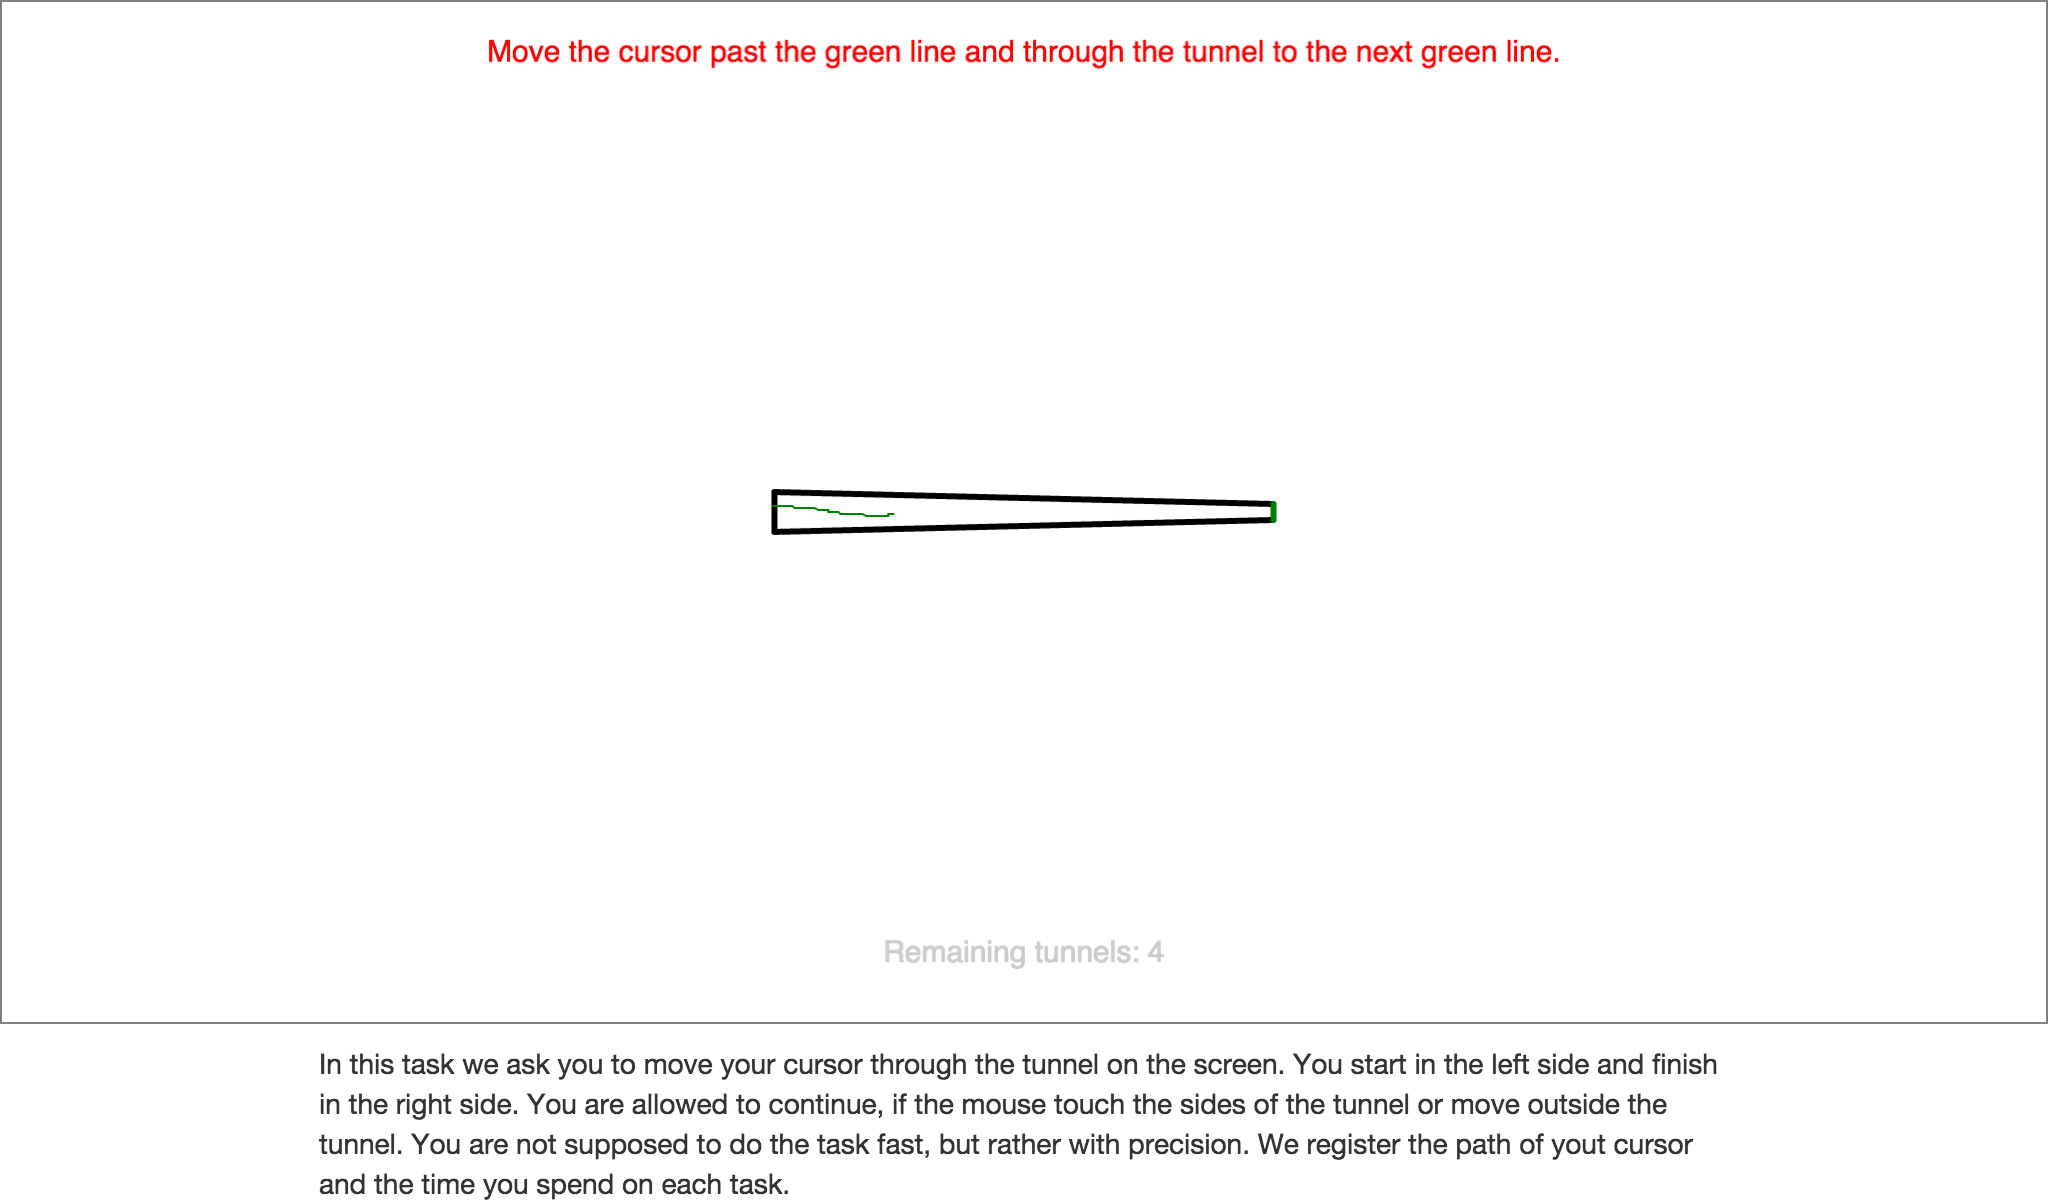
\includegraphics[width=\textwidth, trim = 25cm 15cm 25cm 10cm, clip]{images/screenshots/ex_step_4_tunnel_path}
\label{fig:tunnelopgaver}
\caption{Illustration af spiralopgave}
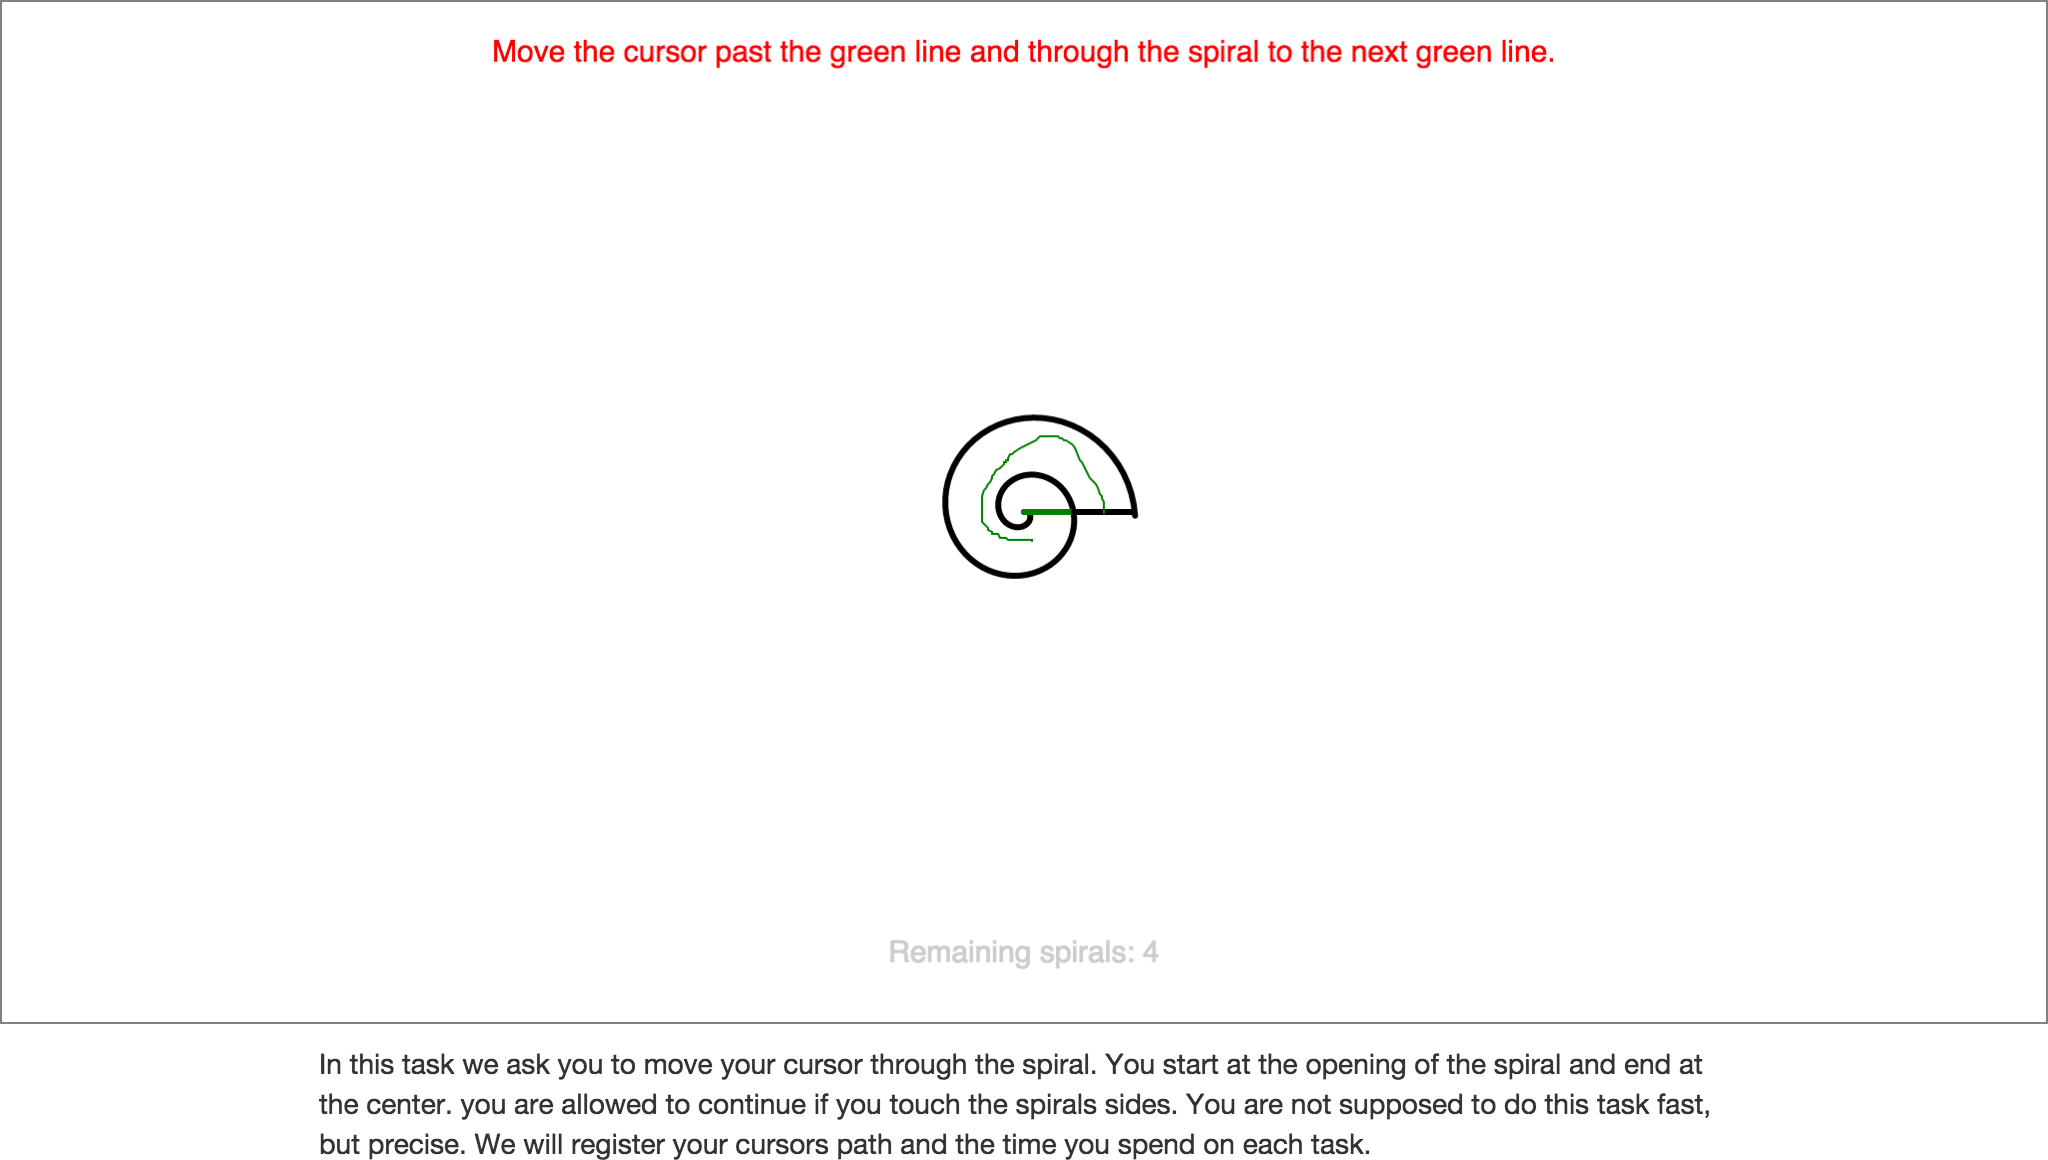
\includegraphics[width=\textwidth, trim = 25cm 15cm 25cm 10cm, clip]{images/screenshots/ex_step_5_spiral_path}
\label{fig:spiralopgave}

\end{minipage}\hfill
\begin{minipage}[t]{.5\textwidth}
\centering
\vspace{0pt}
    \begin{tabular}{ c c c c }
        Forsøg & $A$ & $W$ & $A/W$ \\\hline\hline
        1  & 67  & 20 & 3.35  \\
        2  & 184 & 38 & 4.84  \\
        3  & 280 & 14 & 20.00 \\
        4  & 230 & 29 & 7.93  \\
        5  & 144 & 55 & 2.62  \\
        6  & 249 & 29 & 8.59  \\
        7  & 255 & 14 & 18.21 \\
        8  & 96  & 50 & 1.92  \\
        9  & 225 & 19 & 11.84 \\
        10 & 263 & 12 & 21.92 \\
        11 & 259 & 25 & 10.36 \\
        12 & 229 & 20 & 11.45 \\
        13 & 215 & 31 & 6.94  \\
        14 & 198 & 83 & 2.39  \\
        15 & 301 & 16 & 18.81 \\
        16 & 194 & 66 & 2.94  \\
        17 & 260 & 12 & 21.67 \\
        18 & 296 & 14 & 21.14 \\
        19 & 180 & 44 & 4.09  \\
        20 & 278 & 11 & 25.27 \\
        21 & 283 & 37 & 7.65  \\
        22 & 40  & 32 & 1.25  \\
        23 & 233 & 10 & 23.30 \\
        24 & 191 & 50 & 3.82  \\
        25 & 179 & 18 & 9.94  \\\hline
    \end{tabular}
    \captionof{table}{Afstand og størrelse på målet}\label{tab:pegeopgave}
\end{minipage}

%\addcontentsline{toc}{chapter}{Statistik}
%\chapter*{Statistik}

\newpage
\addcontentsline{toc}{chapter}{Analyse}
\chapter*{Analyse}
\addcontentsline{toc}{section}{Modeludvælgelse}
\section*{Modeludvælgelse}
Som det kan ses af de fire formuleringer for Fitts' lov, så kan de alle sammen opfattes som lineære modeller, med tiden, T, som y-variabel og ID som x-variabel. Bemærk, at Welfords formel har en skæring med y-aksen i 0, dvs. $a=0$. 

For at kunne finde ud af, hvilken af de fire lineære modeller, som beskriver vores data bedst, har vi overvejet følgende sammenligningskriterier.

\begin{itemize}
\item{Least Squared Errors (LSE).}
\item{Mallow's $C_p$.}
\item{Akaike Information Criterion (AIC).}
\item{Bayesian Information Criterion (BIC).}
\end{itemize}

LSE er bestemt ved at finde gennemsnittet af kvadratet på afstandene fra punkterne til modellen, den model som har det laveste gennemsnit bliver vurderet som bedst. Et problem ved udelukkende at benytte dette kriterium er, at en model altid kan beskrive alle data punkter perfekt ved blot at inkludere flere parametre. Dette er hvad der kan klassificeres som overfitting.

Mallow's $C_p$ kriteriet bliver beregnet ud fra LSE men inddrager også antallet af parametre i beregningen for netop at undgå overfitting. Tilsvarende gør sig gældende for AIC og BIC, de beregnes dog ved hjælp af maximum likelihood i stedet for LSE.

For et givent datasæt med parametre og udfald og en tilhørende statistisk model vil likelihood funktionen beregne sandsynligheden for at modellens parametre vil resultere i de givne udfald. Ved maximum likelihood findes de værdier for modellens parametre som maksimere likelihood funktionen, det vil sige har størst sandsynlighed for at hænde. Forskellen imellem AIC og BIC er, at BIC vægter antallet af parametre mere negativt end AIC.

Af de fire beskrevne modeller har vi valgt at bruge AIC, da det er den mest udbredte at basere sin modeludvælgelse på. Hvis vi lader $L$ være maximum likelihood værdierne for modellens parametre og $k$ antallet af parametre, så er AIC givet ved
\begin{align}
AIC = 2k - 2\ln(L)
\end{align}
Vi har til vores analyse brugt programmeringssproget R, som både har lineær regression og AIC funktionalitet indbygget. $lm()$\footnote{R dokumentation om $lm()$: \url{https://stat.ethz.ch/R-manual/R-patched/library/stats/html/lm.html}} fitter en lineær model ud fra de (x,y) datasæt der gives som input. Modellen bliver baseret på least squares, og kan også tvinges til at gå igennem origo (for Welford).

$AIC()$\footnote{R dokumentation om $AIC()$: \url{https://stat.ethz.ch/R-manual/R-patched/library/stats/html/AIC.html}} bruger (13) som udgangspunkt til sine beregninger, og tager som input en model, der har metoden $logLik()$\footnote{R dokumentation om $logLik()$: \url{https://stat.ethz.ch/R-manual/R-patched/library/stats/html/logLik.html}}, hvilket $lm()$'s output-modeller har. $lm()$ og $AIC()$ gør det derfor muligt at sammenligne modellerne med R.

\addcontentsline{toc}{section}{Indledende analyse}
\section*{Indledende analyse}
For at være sikre på, at vores data kan bruges til at sammenligne de fire formuleringer har vi først kigget på vores 10 testdeltagere hver for sig. Vi har fitted vores 10 testdeltageres data fra pegeopgaverne til Fitts lov hver for sig. Tre af disse plots kan ses i appendiks D, Testpersonernes individuelle grafer.  Det kan på graferne ses hvordan punkterne ligger pænt omkring modellen, angivet ved den blå linje. Men også, at enkelte datapunkter bryder tendensen, specielt på figur \ref{fig:testdeltager1}. 

På grund af den primært pæne model kan det konkluderes, at vores data godt kan danne grundlag for vores analyse, der kan dog opstå et behov for at skære ekstremt afvigende data fra. Specielt fordi crowdsourcingforsøget er ukontrolleret.

\addcontentsline{toc}{section}{Modelanalyse}
\section*{Modelanalyse}
Vores modelanalyse tager udgangspunkt i AIC-metoden som beskrevet i forrige afsnit, og vi benytter os af de data der er indsamlet ved crowdsourcingdeltagernes udførsel af pegeopgaven.

\addcontentsline{toc}{subsection}{R-kode}
\subsection*{R-kode}
Den relevante R-kode som bliver brugt til analysen, er vist i listing \ref{lst:fitt}, \ref{lst:welford}, \ref{lst:mackenzie}, \ref{lst:meyer}, \ref{lst:aic}.

\lstinputlisting[label={lst:fitt}, caption=Fitt's Modelanalyse, language=R, firstline=38, lastline=45]{analyse.r}
\lstinputlisting[label={lst:welford}, caption=Welford's Modelanalyse, language=R, firstline=47, lastline=54]{analyse.r}
\lstinputlisting[label={lst:mackenzie}, caption=MacKenzie's Modelanalyse, language=R, firstline=56, lastline=63]{analyse.r}
\lstinputlisting[label={lst:meyer}, caption=Meyer's Modelanalyse, language=R, firstline=65, lastline=72]{analyse.r}
\lstinputlisting[label={lst:aic}, caption=AIC-analyse, language=R, firstline=77, lastline=83]{analyse.r}

Som det ses af listing \ref{lst:fitt}, udregner vi først $ID$ for vores data, baseret på de foruddefinerede værdier af $A$ og $W$. Herefter bruger vi $lm()$ til at fitte modellen til vores data, hvorefter vi plotter dataen og modellen i et residualplot.\\
I listing \ref{lst:aic} ses det at vi benytter $AIC()$ på alle fire modeller, hvorefter de bliver sorteret efter størrelse for nemmere sammenligning.

\addcontentsline{toc}{subsection}{Residualanalyse}
\subsection*{Residualanalyse}
\begin{minipage}{\textwidth}
	\centering
	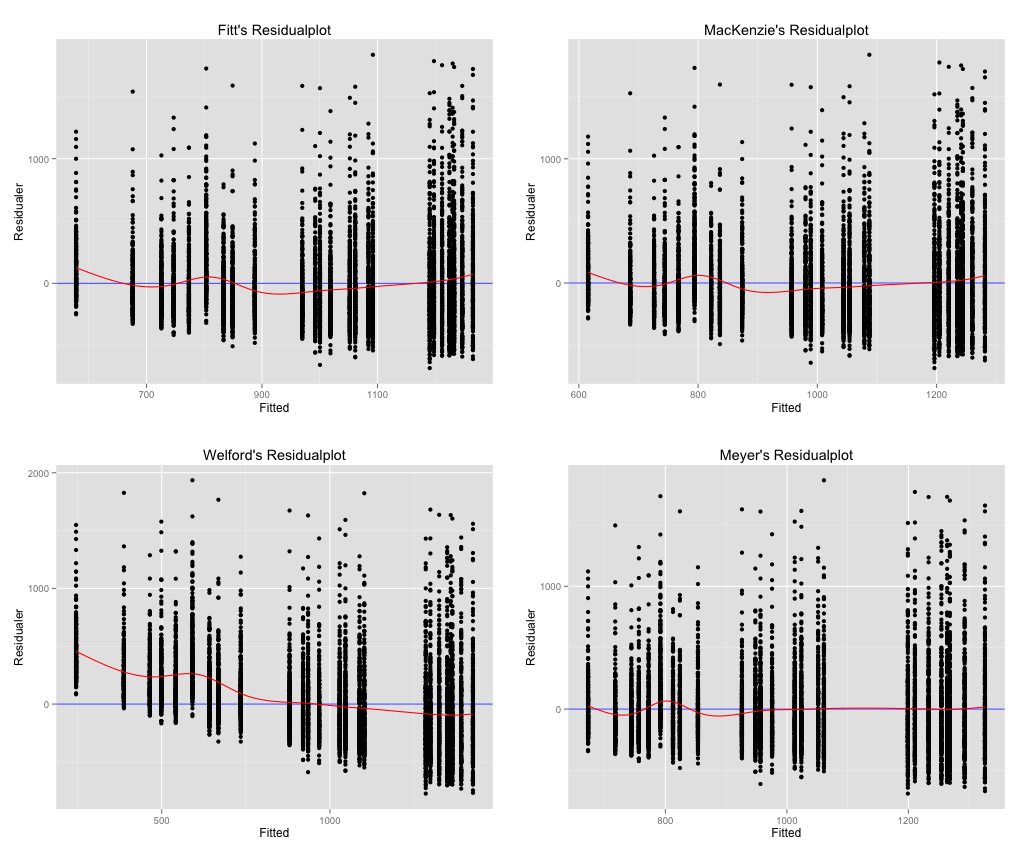
\includegraphics[width=\textwidth]{images/plots/plot_residual_comparison}
	\captionof{figure}{Sammenligning af residualplots}
	\label{fig:plot_residual_comparison}
\end{minipage}\\\\
For at vurdere præcisionen af modellerne, har vi valgt at lave en residualanalyse ved hjælp af residualplots (figur \ref{fig:plot_residual_comparison}). Residualerne I modellerne er variationen i tid ($MT$) som modellerne ikke når at opfange, og de kan derved sige noget om hvor præcis modellerne er i forhold til den data vi har indsamlet.\\
På figur \ref{fig:plot_residual_comparison} ses alle fire modellers residualplot, med en rød linje defineret af en smoothing-funktion. Smoothing-funktionen er tilføjet som et visuelt hjælpemiddel der tydeligt kan vise hvordan residualerne fordeler sig omkring x-aksen. Jo mere centreret de er om aksen, og jo mere linære de er i forhold til aksen, jo bedre er modellen.\\
Vi kan derfor hurtigt se på Welford's residualplot at denne model passer dårligt på vores data, hvorom Fitt's, MacKenzie's og Meyer's ligger sig tættere op ad den data vi har indsamlet - det ses ved nærmere studering at smoothing-funktionen's linje at Meyer's model giver os det bedste fit til vores data.


\addcontentsline{toc}{subsection}{AIC-analyse}
\subsection*{AIC-analyse}
\begin{minipage}{\textwidth}
	\centering
	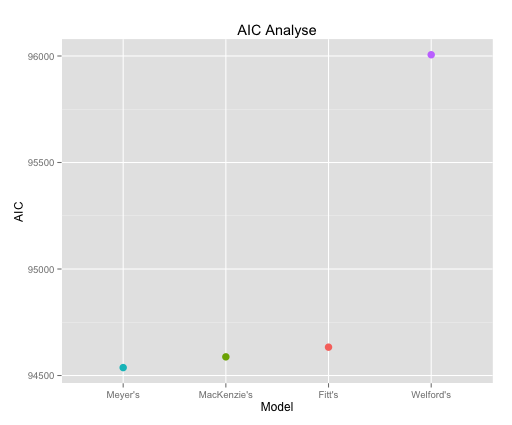
\includegraphics[width=.75\textwidth]{images/plots/plot_analysis_aic}
	\captionof{figure}{AIC-analyse}
	\label{fig:plot_analysis_aic}
\end{minipage}\\\\
Bla bla bla.. tekst om residualanalyse

%\addcontentsline{toc}{chapter}{Konklusion}
%\chapter*{Konklusion}

\nocite{*}
\newpage
\begin{appendices}

%-- Drejebog --%
\chapter{Drejebog for laboratorieeksperiment}
\label{sec:drejebog}
\subsection*{Udstyr}
\begin{itemize}
\item{Computer med Google Chrome browseren}
\item{Mus og musemåtte}
\end{itemize}
\subsection*{Før test}
\begin{itemize}
\item{P1 rækker testdeltager et A4 ark med følgende tekst;
      \\\textit{"Vi er i gang med et bachelorprojekt, der handler om Fitts' lov. Det er en model, som beskriver det menneskelige motoriske systems kapacitet. I denne sammenhæng, hvordan tiden til at ramme et mål på skærmen ved hjælp af musen afhænger af afstanden til og størrelsen på målet. Vi har derfor udviklet dette eksperiment for at indsamle data. Du vil undervejs blive stillet forskellige opgaver, som du skal forsøge at løse."}}
\item{P1 beder testdeltageren om at teste musens følsomhed ved at køre frit rundt med musen. Der gøres opmærksom på, at testdeltageren gerne må ændre følsomheden, hvis de føler for det.}
\item{P2 starter en Google Chrome browser og peger den på følgende adresse:\\ \url{http://codeit.io/bachelor/survey.html}.}
\end{itemize}
\subsection*{Under test}
\begin{itemize}
\item{P2 beder testdeltageren om at tage plads ved den klargjorte computer.}
\item{P2 beder testdeltageren om at udfylde formularen på skærmen med information.}
\item{P2 gør opmærksom på, at der skal skrives 'testperson x', hvor 'x' er nummeret på testpersonen, i feltet om hvorfra de hørte om siden (dette er for senere at kunne finde dem i databasen)}
\item{P1 fortæller testdeltageren, at de gerne må gå i gang med opgaverne og kan stille spørgsmål undervejs, hvis de har brug for det.}
\end{itemize}
\subsection*{Efter test}
\begin{itemize}
\item{P1 fortæller testdeltageren, hvordan  deres data vil blive brugt;
\\\textit{"Tak fordi du ville deltage i forsøget og hjælpe os med vores projekt. De baner du undervejs har foretaget for at udføre opgaverne vil blive brugt til at analysere, hvorvidt de stemmer overens med forskellige formuleringer af Fitt's lov, eller om der kan findes en forbedret formulering"}.}
\end{itemize}

%-- Tekst til crowdsourcing --%
\chapter{Tekst til crowdsourcing}
\label{sec:crowdsource-text}
For at crowdsource vores eksperiment har vi delt følgende tekst:
\\\\\textit{"Hej,\\ vi er tre datalogi studerende ved Københavns Universitet, som er i gang med vores bacheloropgave. For at kunne have nogle data at analysere, har vi lavet denne hjemmeside med 'pegeopgaver'. Opgaverne tager cirka 10-15 minutter at udføre og er skidesjove! Det ville derfor være utrolig værdsat, hvis du ville gå ind på følgende hjemmeside \url{http://www.codeit.io/bachelor/index.html} og udføre opgaverne. Deltag senest d. 27/04.
\\Eventulle spørgsmål kan henvendes til en af os på;\\bdj816@alumni.ku.dk, hmd200@alumni.ku.dk, qgf142@alumni.ku.dk"}
\\\\\textit{"Hello,\\ We are three computer science students at the University of Copenhagen, who are currently working on our bachelor thesis. We have made the following webpage with 'pointingtasks' in order to have some data to analyze. The tasks takes approximately 10-15 minuttes and are super fun! It would therefore be very appreciated if you would visit the webpage at \url{http://www.codeit.io/bachelor/index.html} and complete the tasks. Deadline is the 27th of April.
\\Any questions regarding the projects are welcome at either of these emails;\\bdj816@alumni.ku.dk, hmd200@alumni.ku.dk, qgf142@alumni.ku.dk"}

%-- Skærmbilleder af eksperiment --%
\chapter{Skærmbilleder af eksperiment}
\label{sec:screenshots}
\begin{minipage}{\textwidth}
\centering

\includegraphics[width=\textwidth]{images/screenshots/ex_step_1_intro}
\captionof{figure}{Eksperiment - Trin 1 - Intro}
\label{fig:ex_step_1_intro}
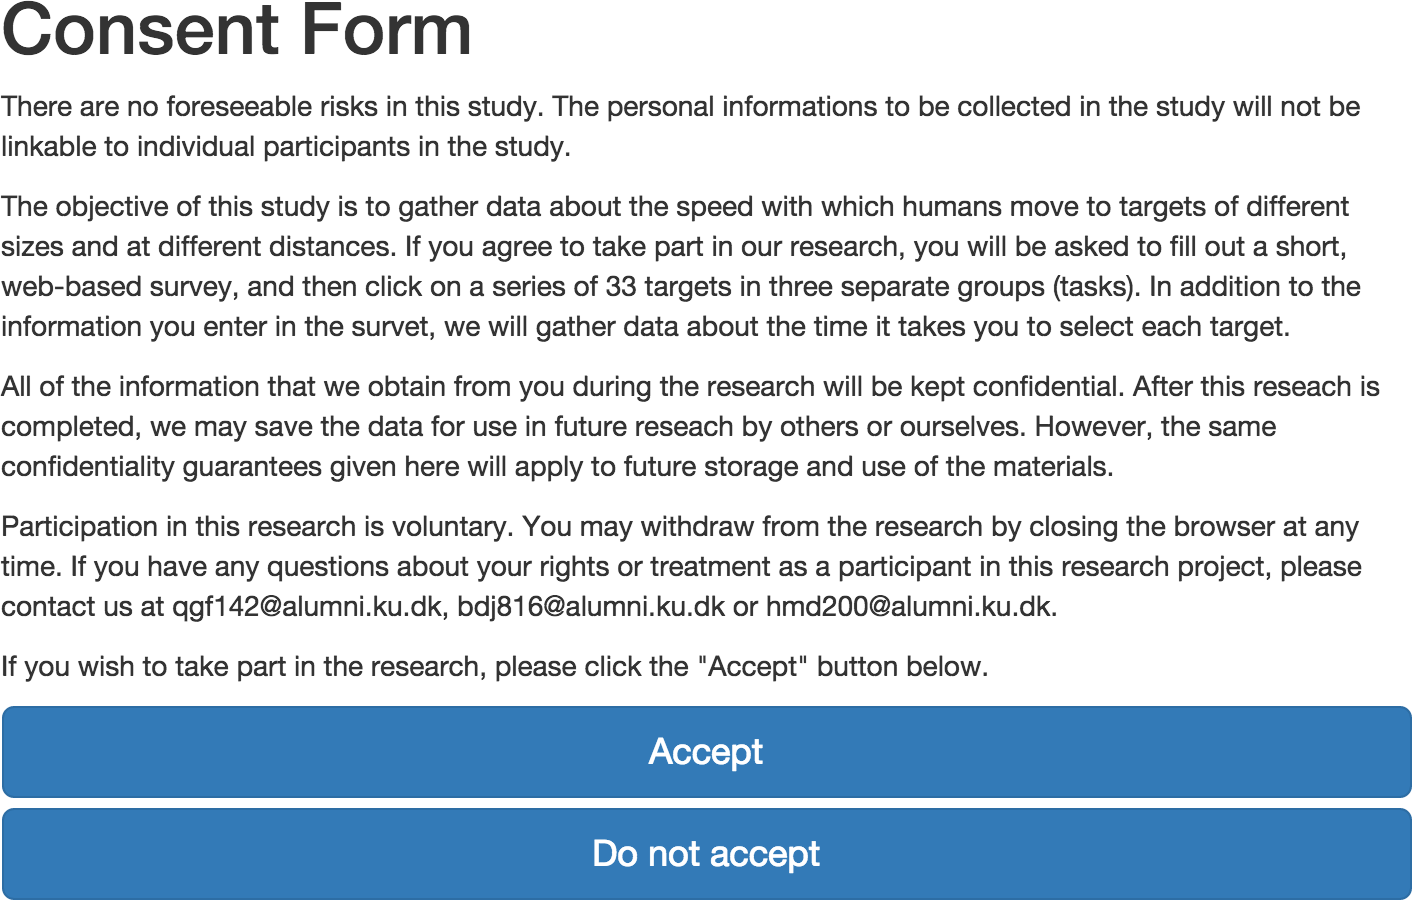
\includegraphics[width=\textwidth]{images/screenshots/ex_step_2_consent}
\captionof{figure}{Eksperiment - Trin 2 - Samtykke}
\label{fig:ex_step_2_consent}
\end{minipage}

\begin{minipage}{\textwidth}
\centering
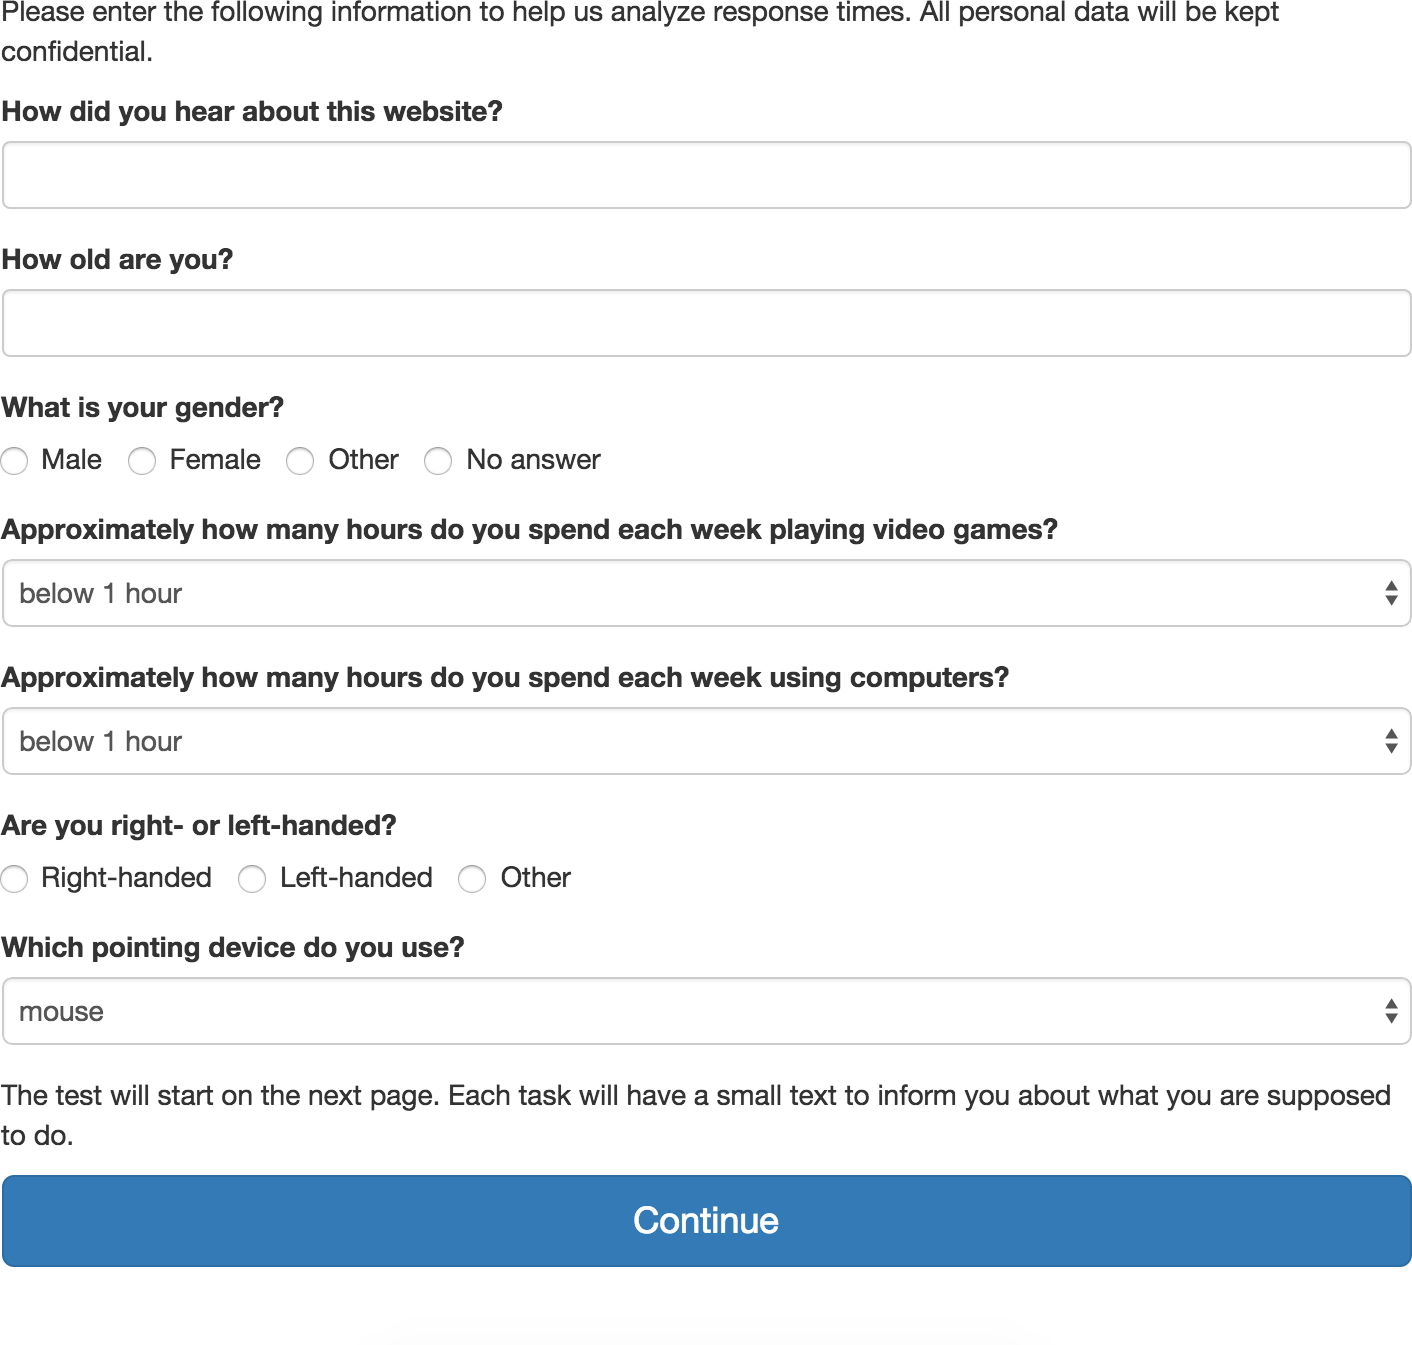
\includegraphics[width=\textwidth]{images/screenshots/ex_step_3_questions}
\captionof{figure}{Eksperiment - Trin 3 - Spørgsmål}
\label{fig:ex_step_3_questions}
\end{minipage}

\begin{minipage}{\textwidth}
\centering
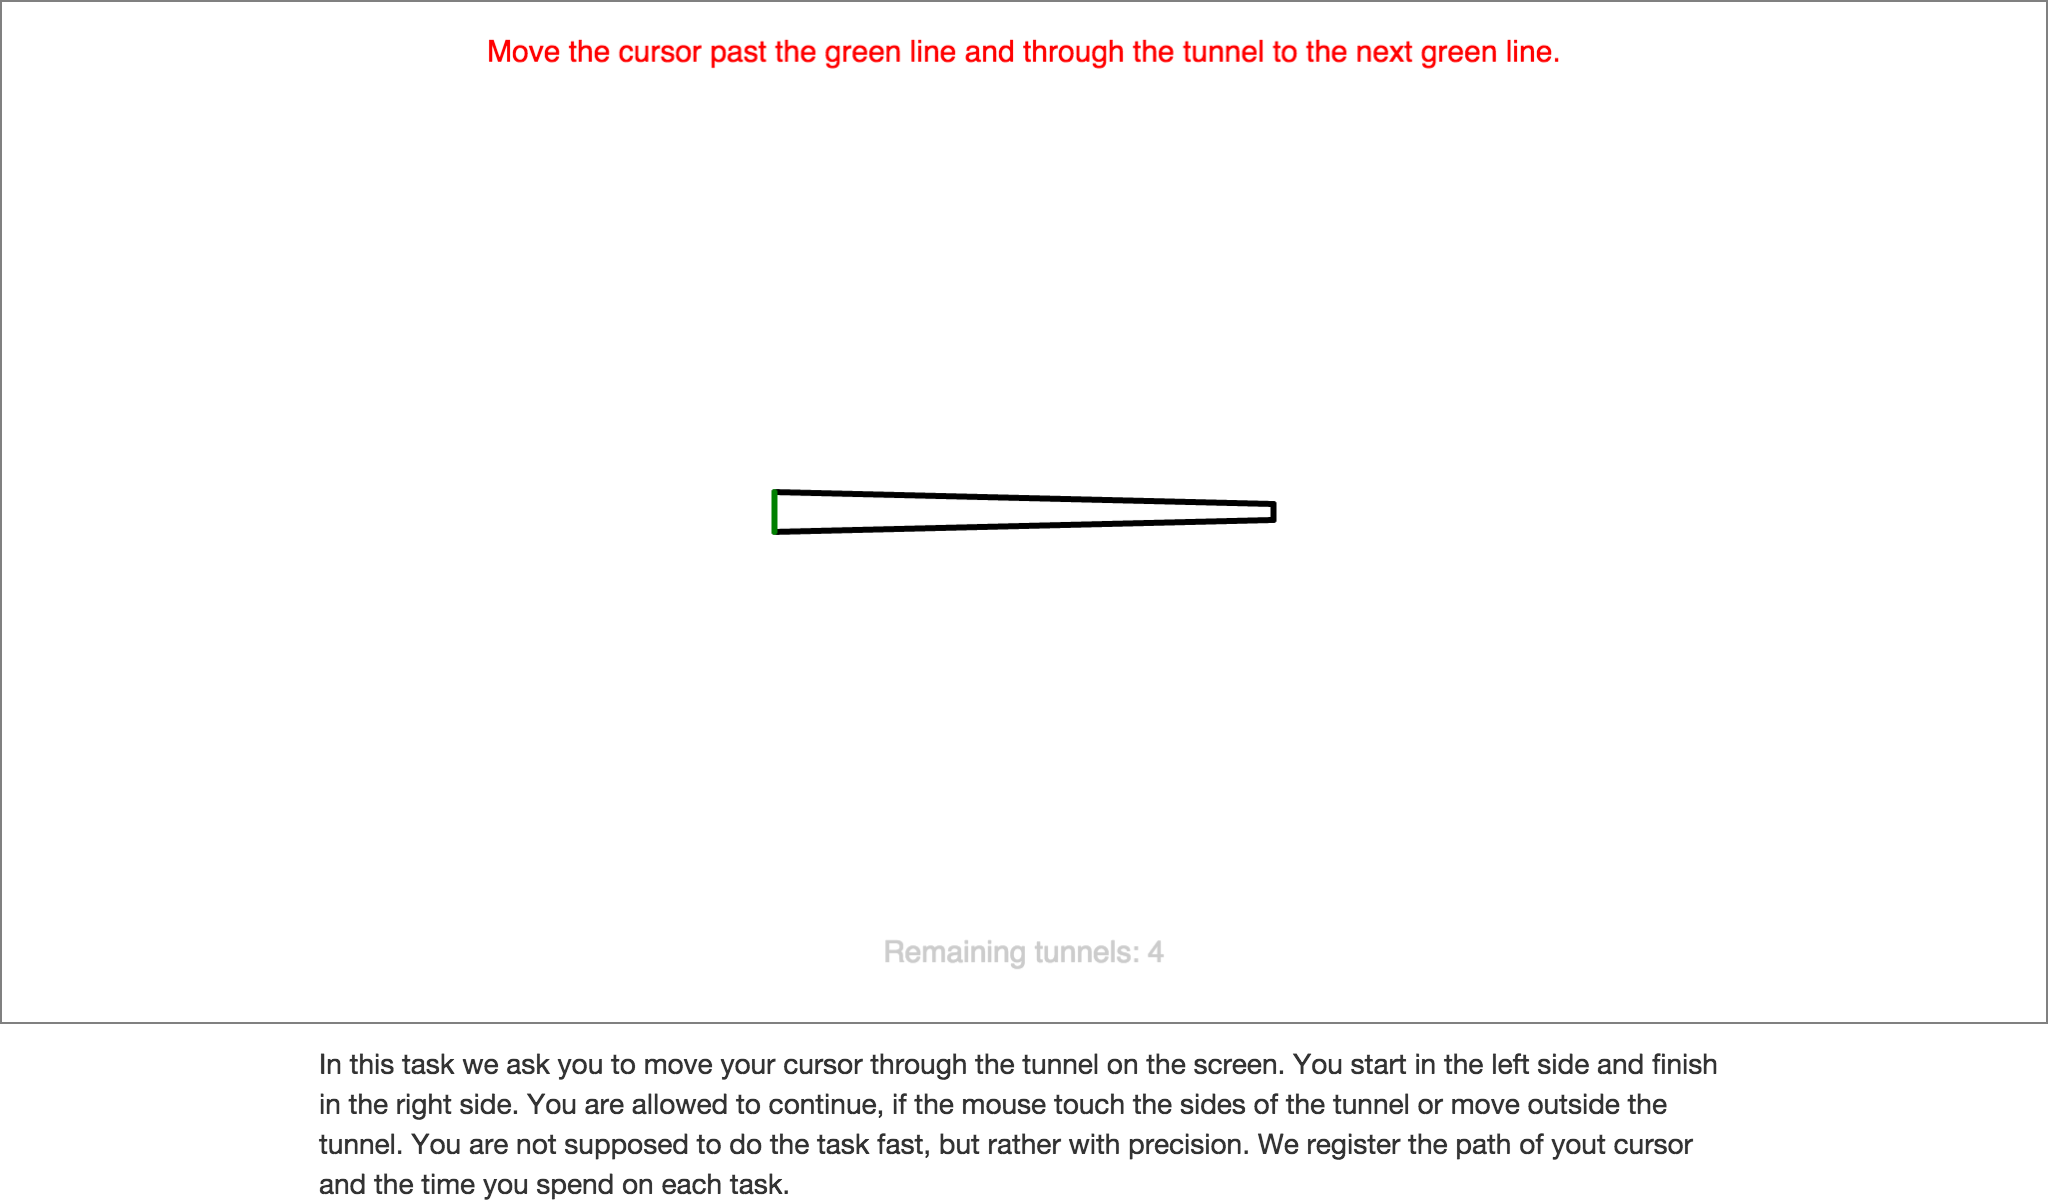
\includegraphics[width=\textwidth]{images/screenshots/ex_step_4_tunnel_1}
\captionof{figure}{Eksperiment - Trin 4 - Tunnel 1}
\label{fig:ex_step_4_tunnel_1}
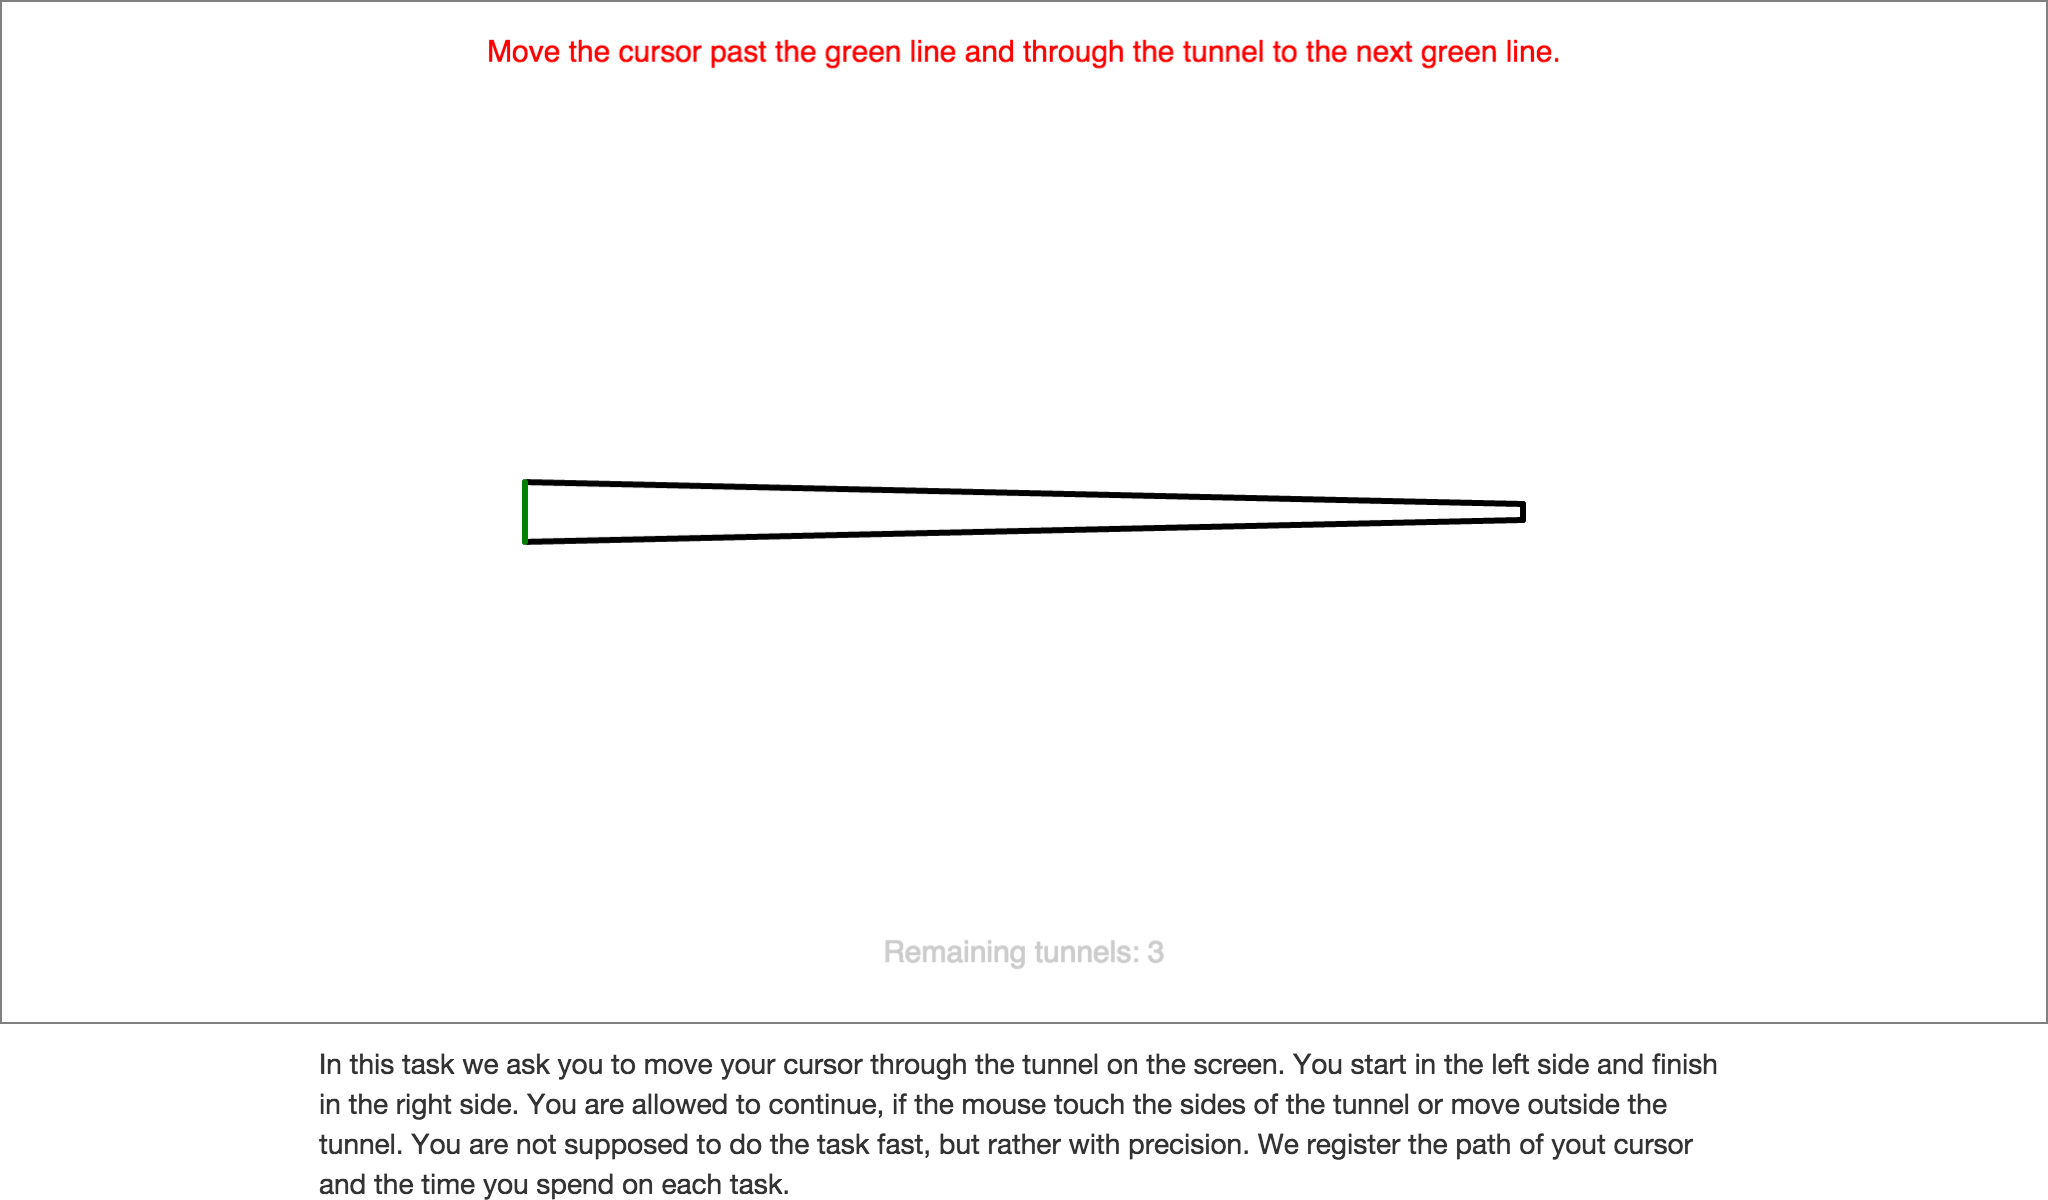
\includegraphics[width=\textwidth]{images/screenshots/ex_step_4_tunnel_2}
\captionof{figure}{Eksperiment - Trin 4 - Tunnel 2}
\label{fig:ex_step_4_tunnel_2}
\end{minipage}

\begin{minipage}{\textwidth}
\centering
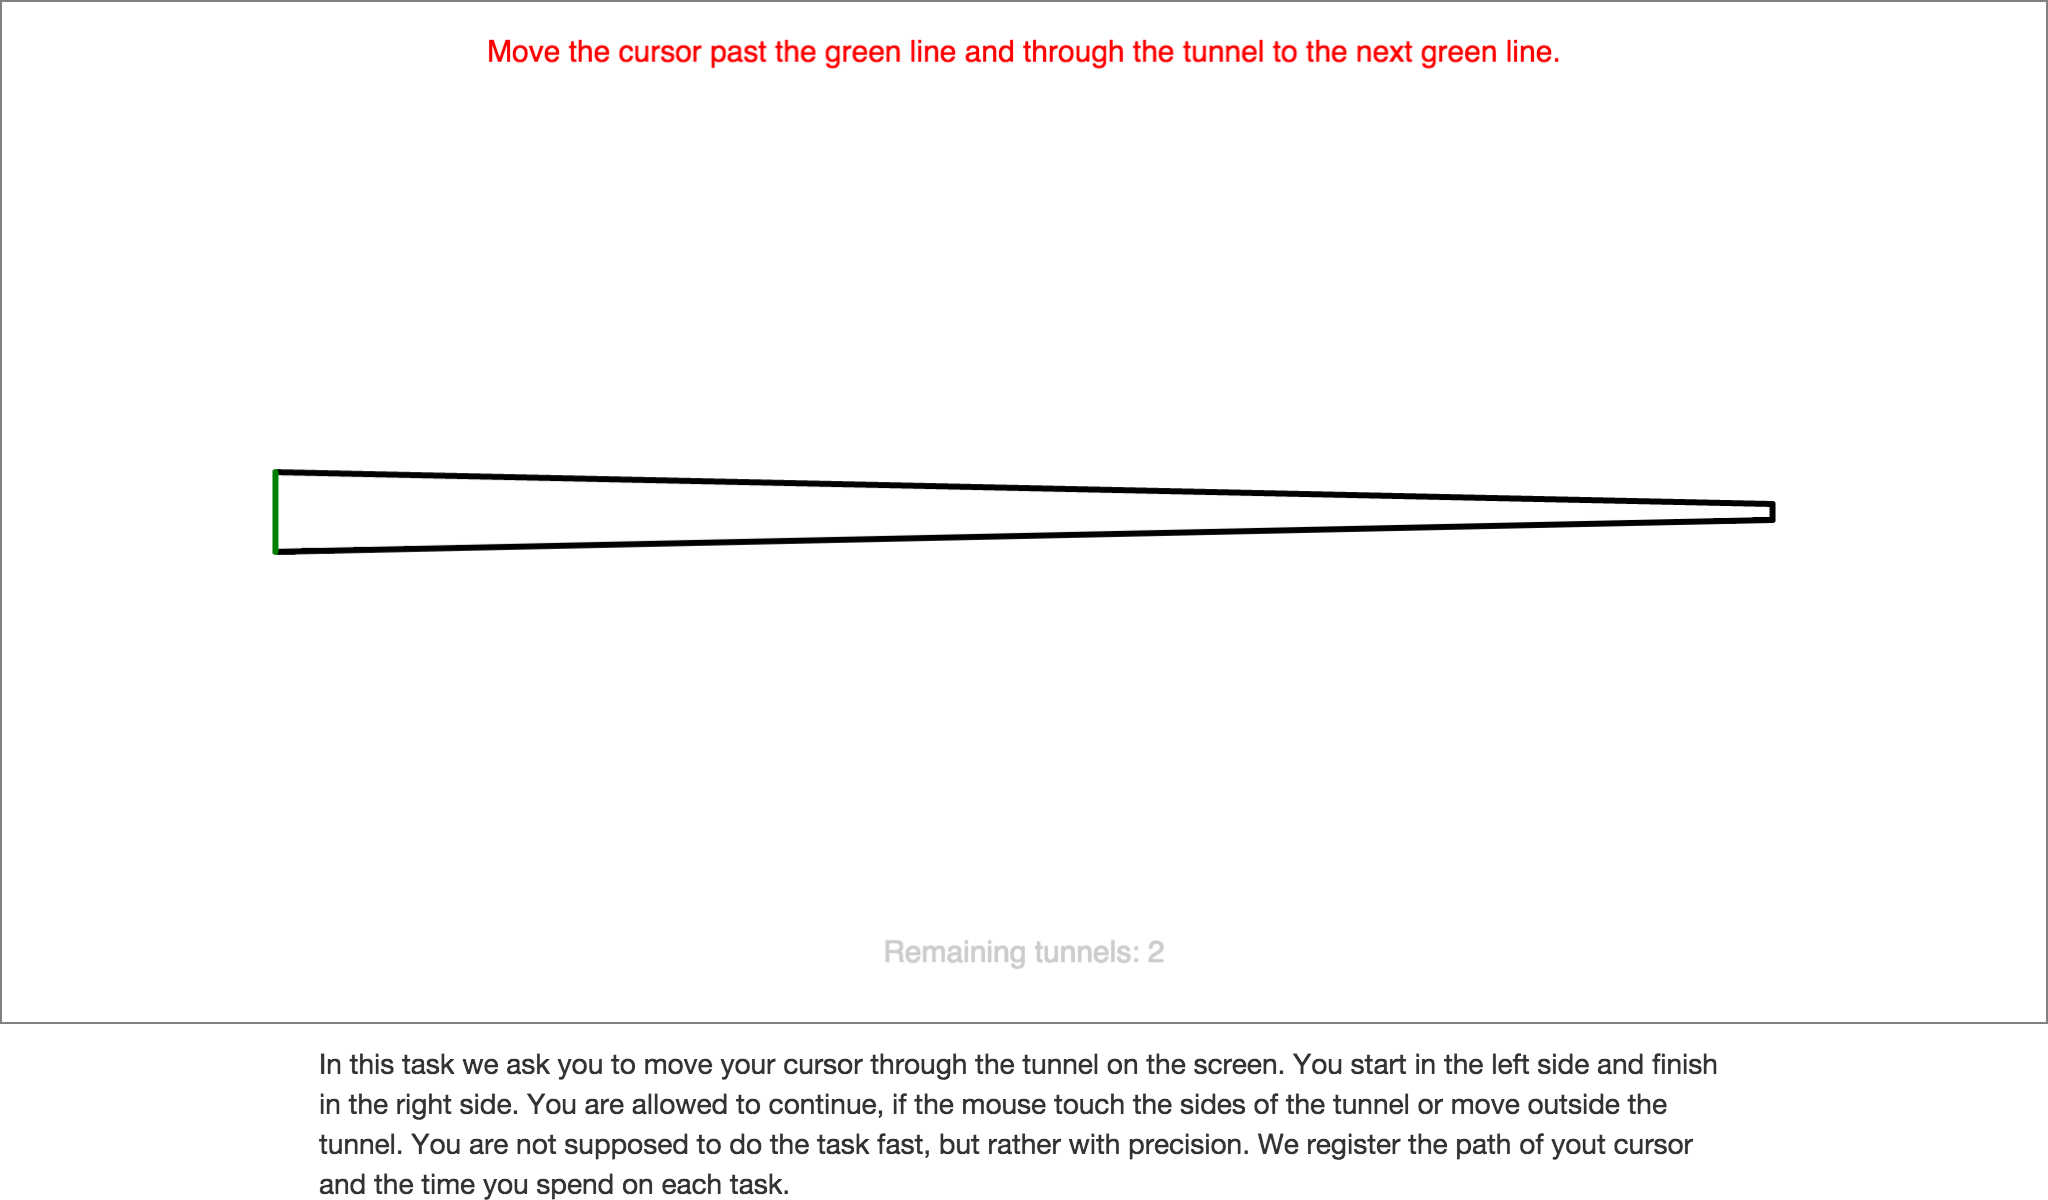
\includegraphics[width=\textwidth]{images/screenshots/ex_step_4_tunnel_3}
\captionof{figure}{Eksperiment - Trin 4 - Tunnel 3}
\label{fig:ex_step_4_tunnel_3}
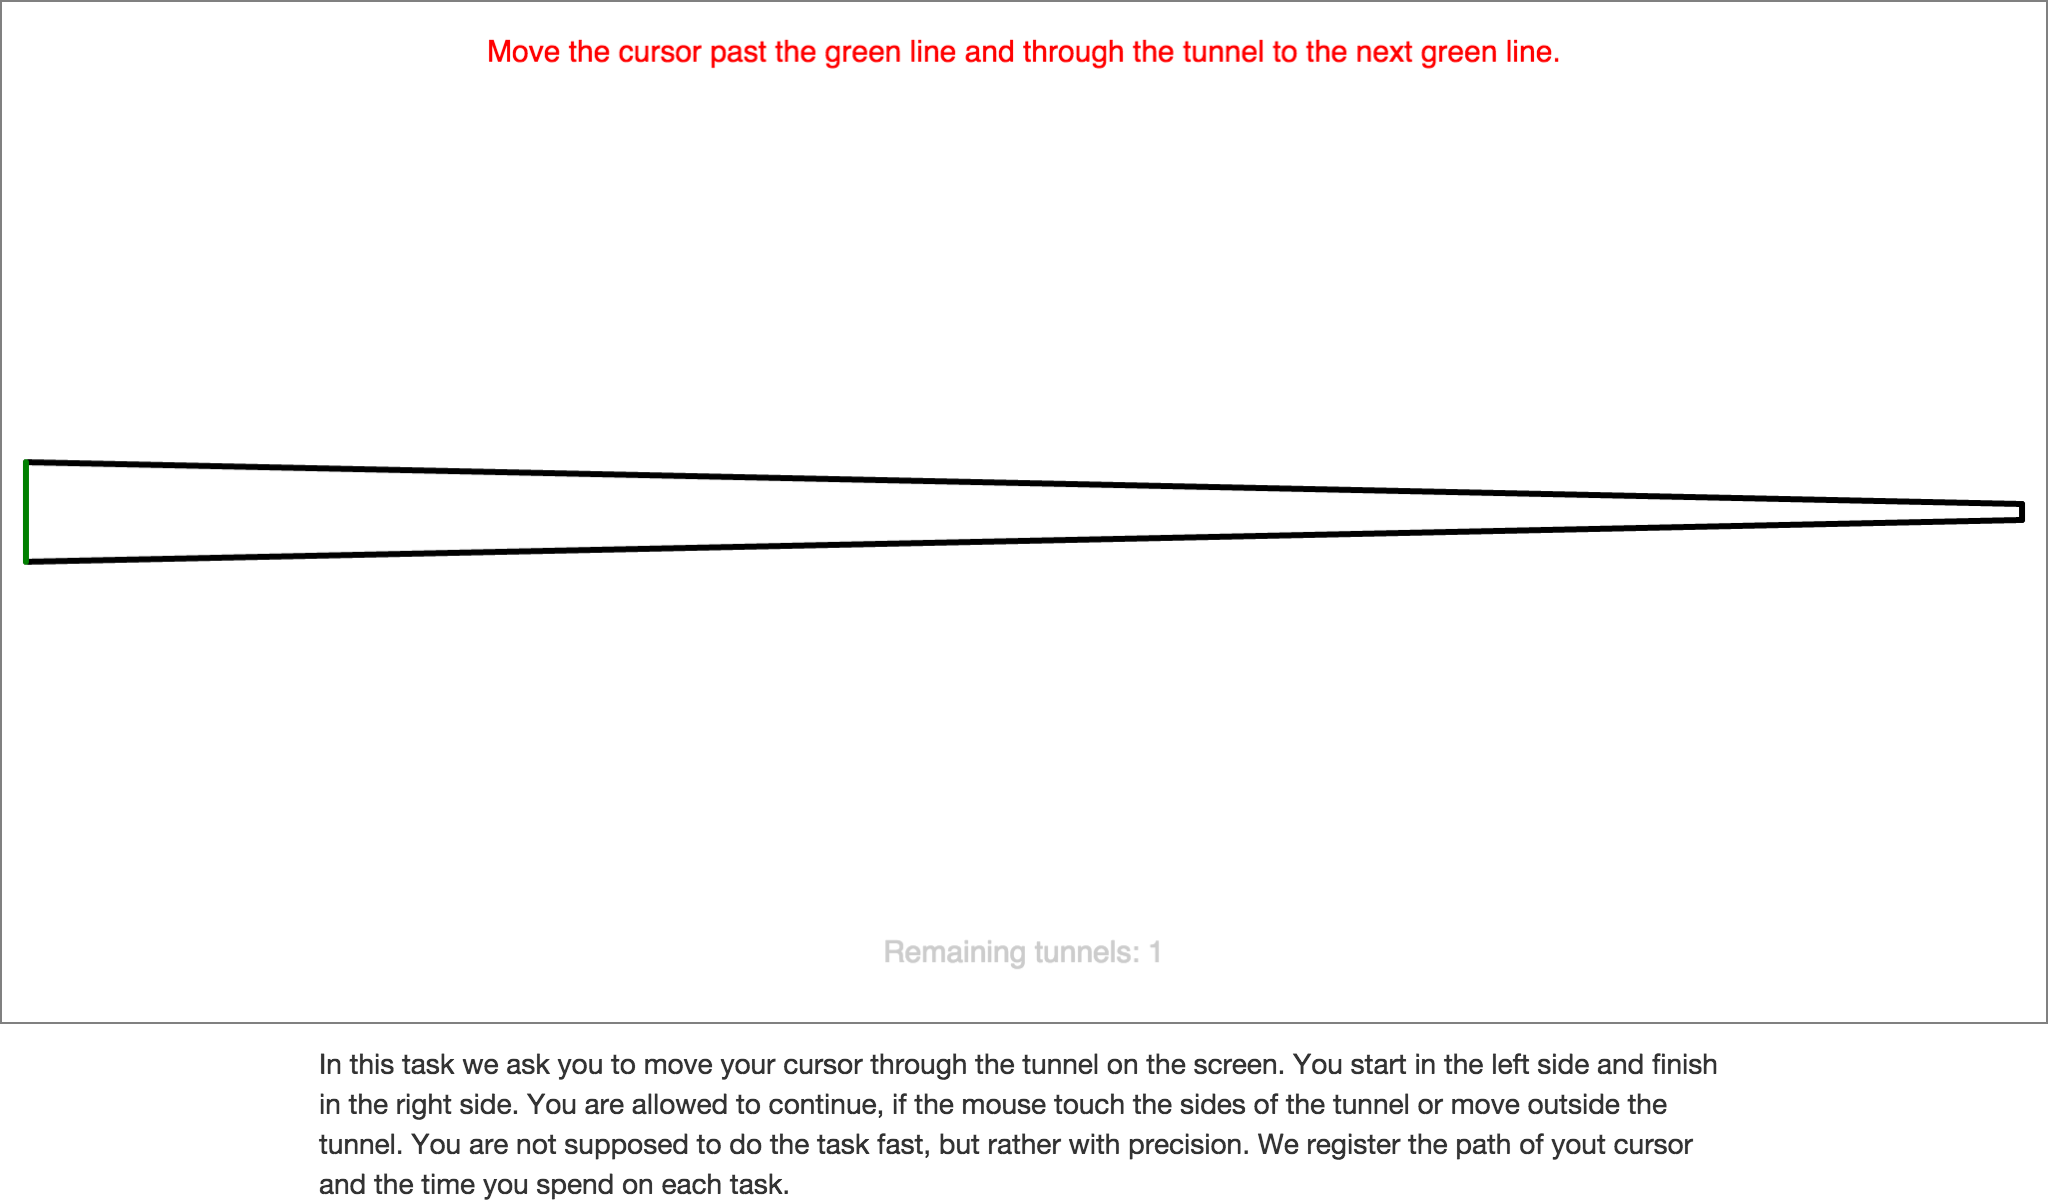
\includegraphics[width=\textwidth]{images/screenshots/ex_step_4_tunnel_4}
\captionof{figure}{Eksperiment - Trin 4 - Tunnel 4}
\label{fig:ex_step_4_tunnel_3}
\end{minipage}

\begin{minipage}{\textwidth}
\centering
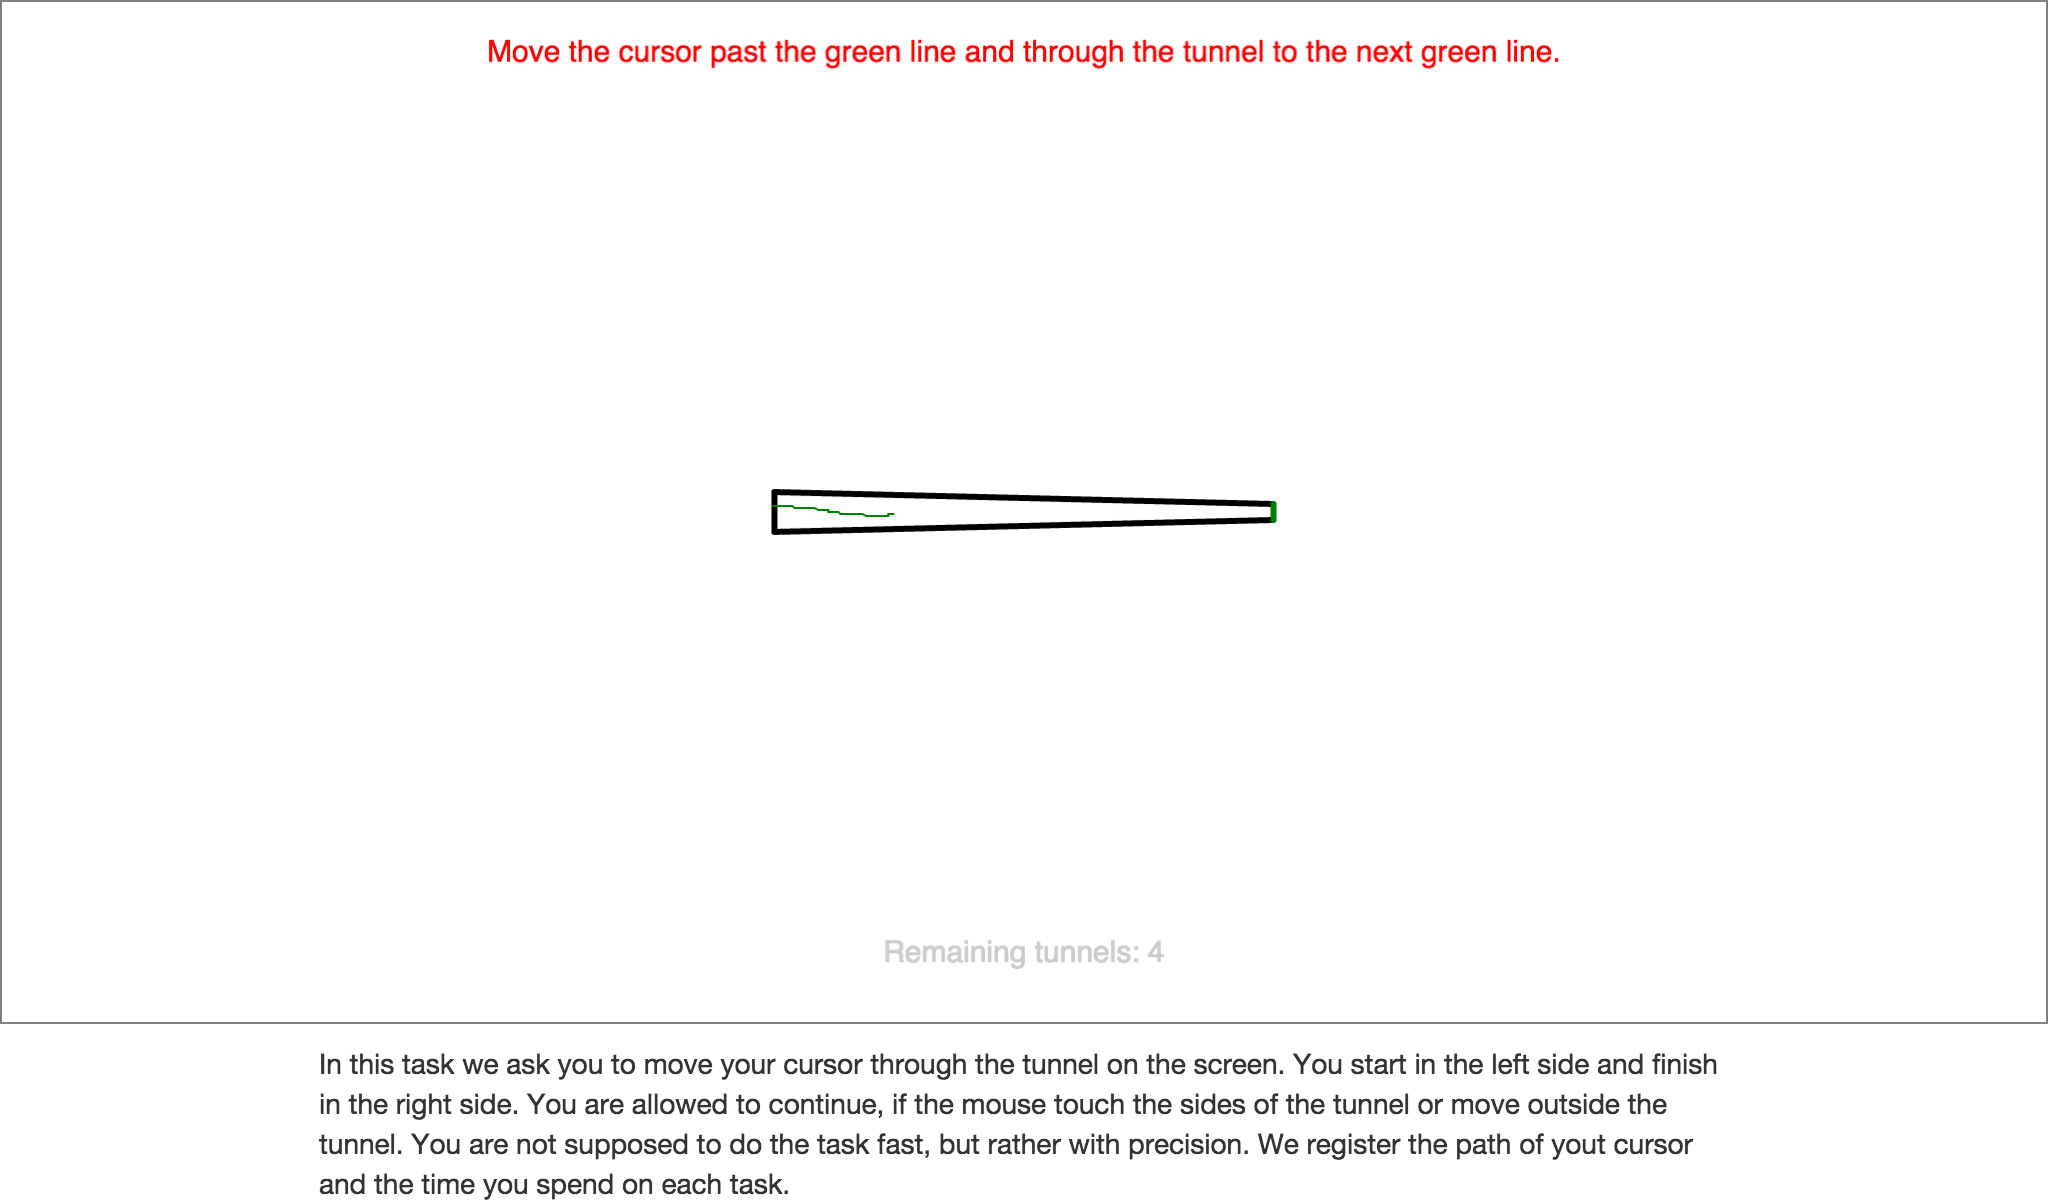
\includegraphics[width=\textwidth]{images/screenshots/ex_step_4_tunnel_path}
\captionof{figure}{Eksperiment - Trin 4 - Tunnelbane}
\label{fig:ex_step_4_tunnel_path}
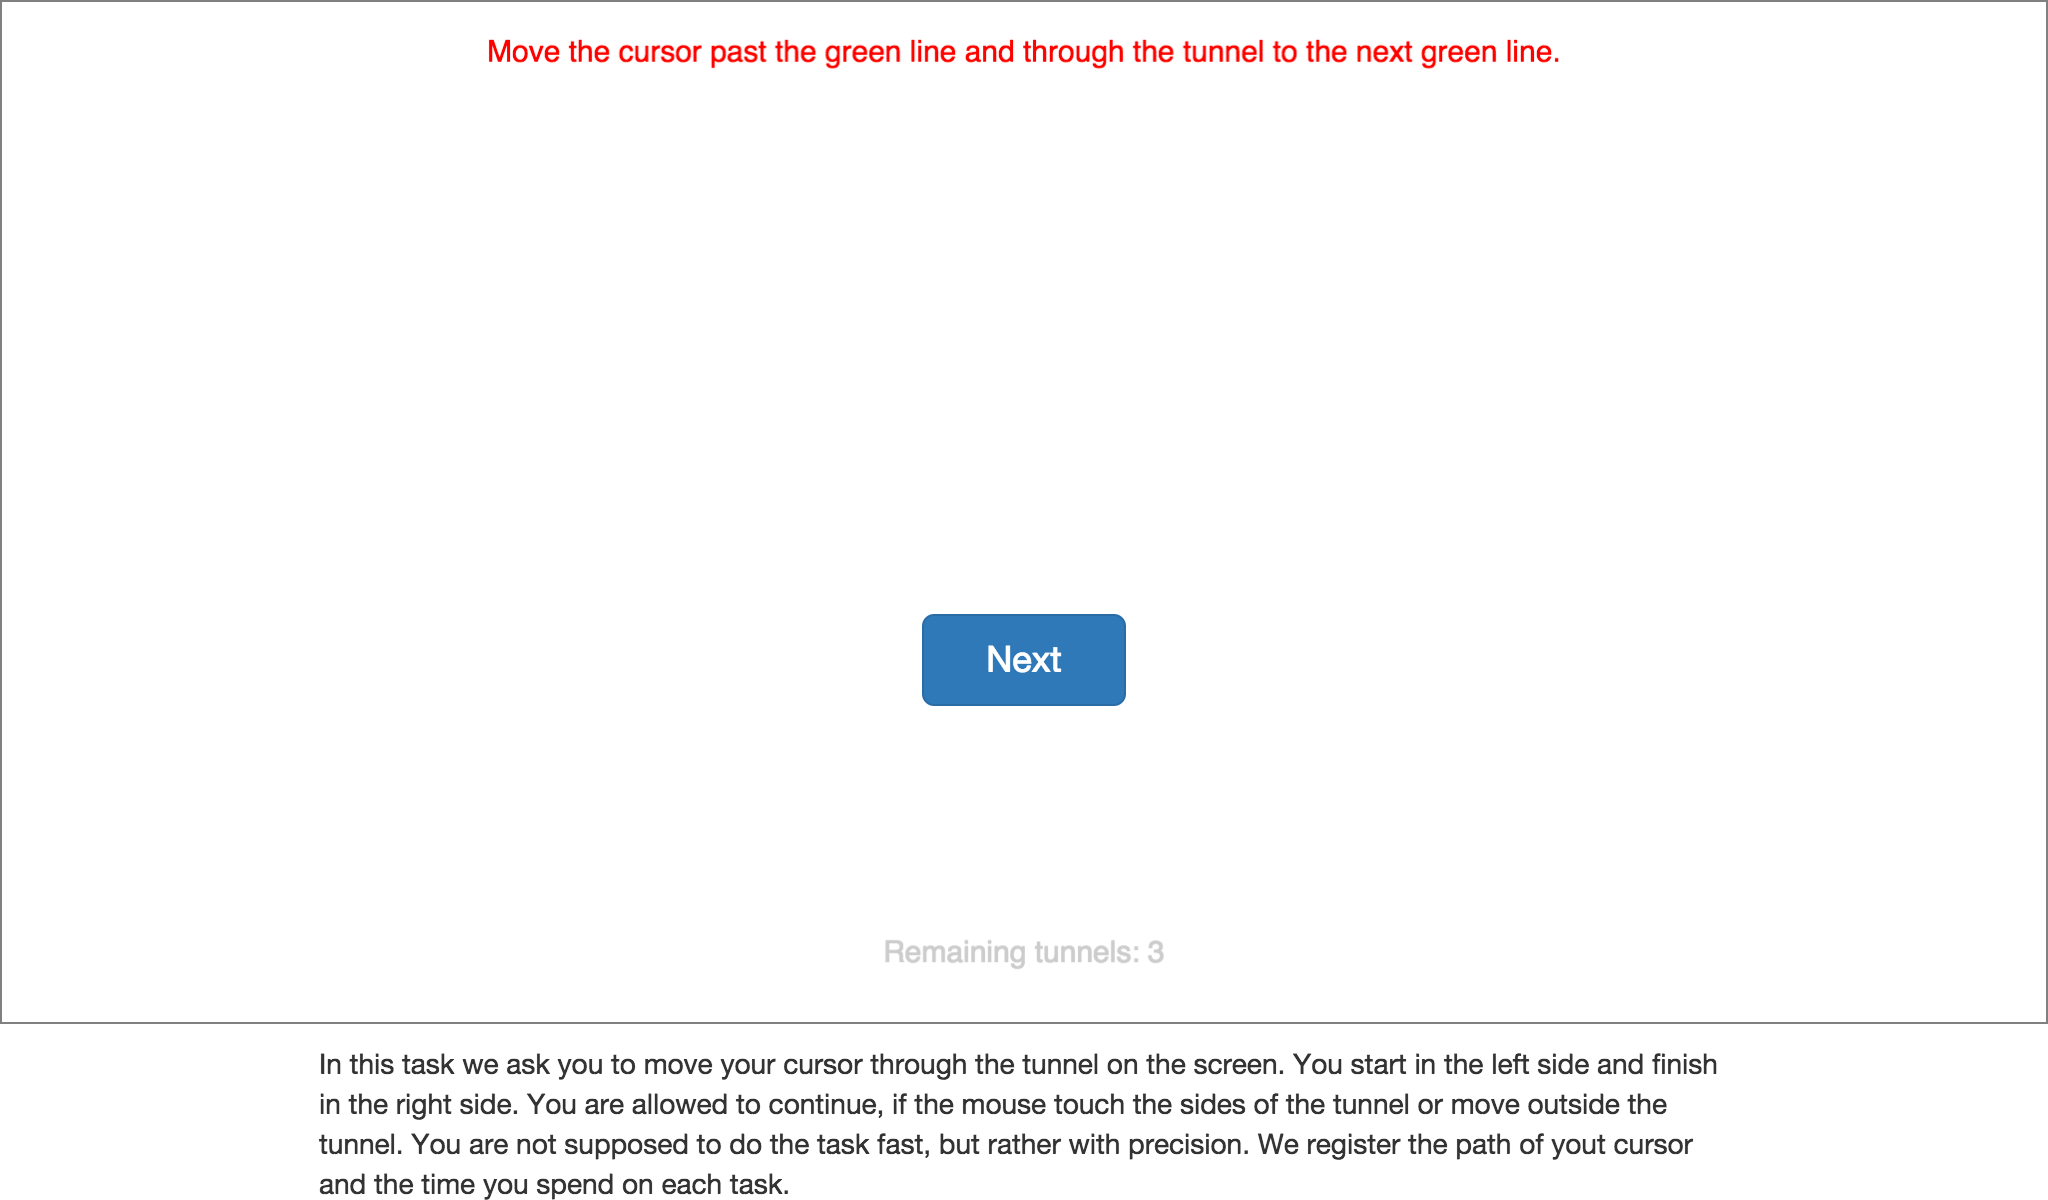
\includegraphics[width=\textwidth]{images/screenshots/ex_step_4_tunnel_next}
\captionof{figure}{Eksperiment - Trin 4 - Næste tunnel}
\label{fig:ex_step_4_tunnel_next}
\end{minipage}

\begin{minipage}{\textwidth}
\centering
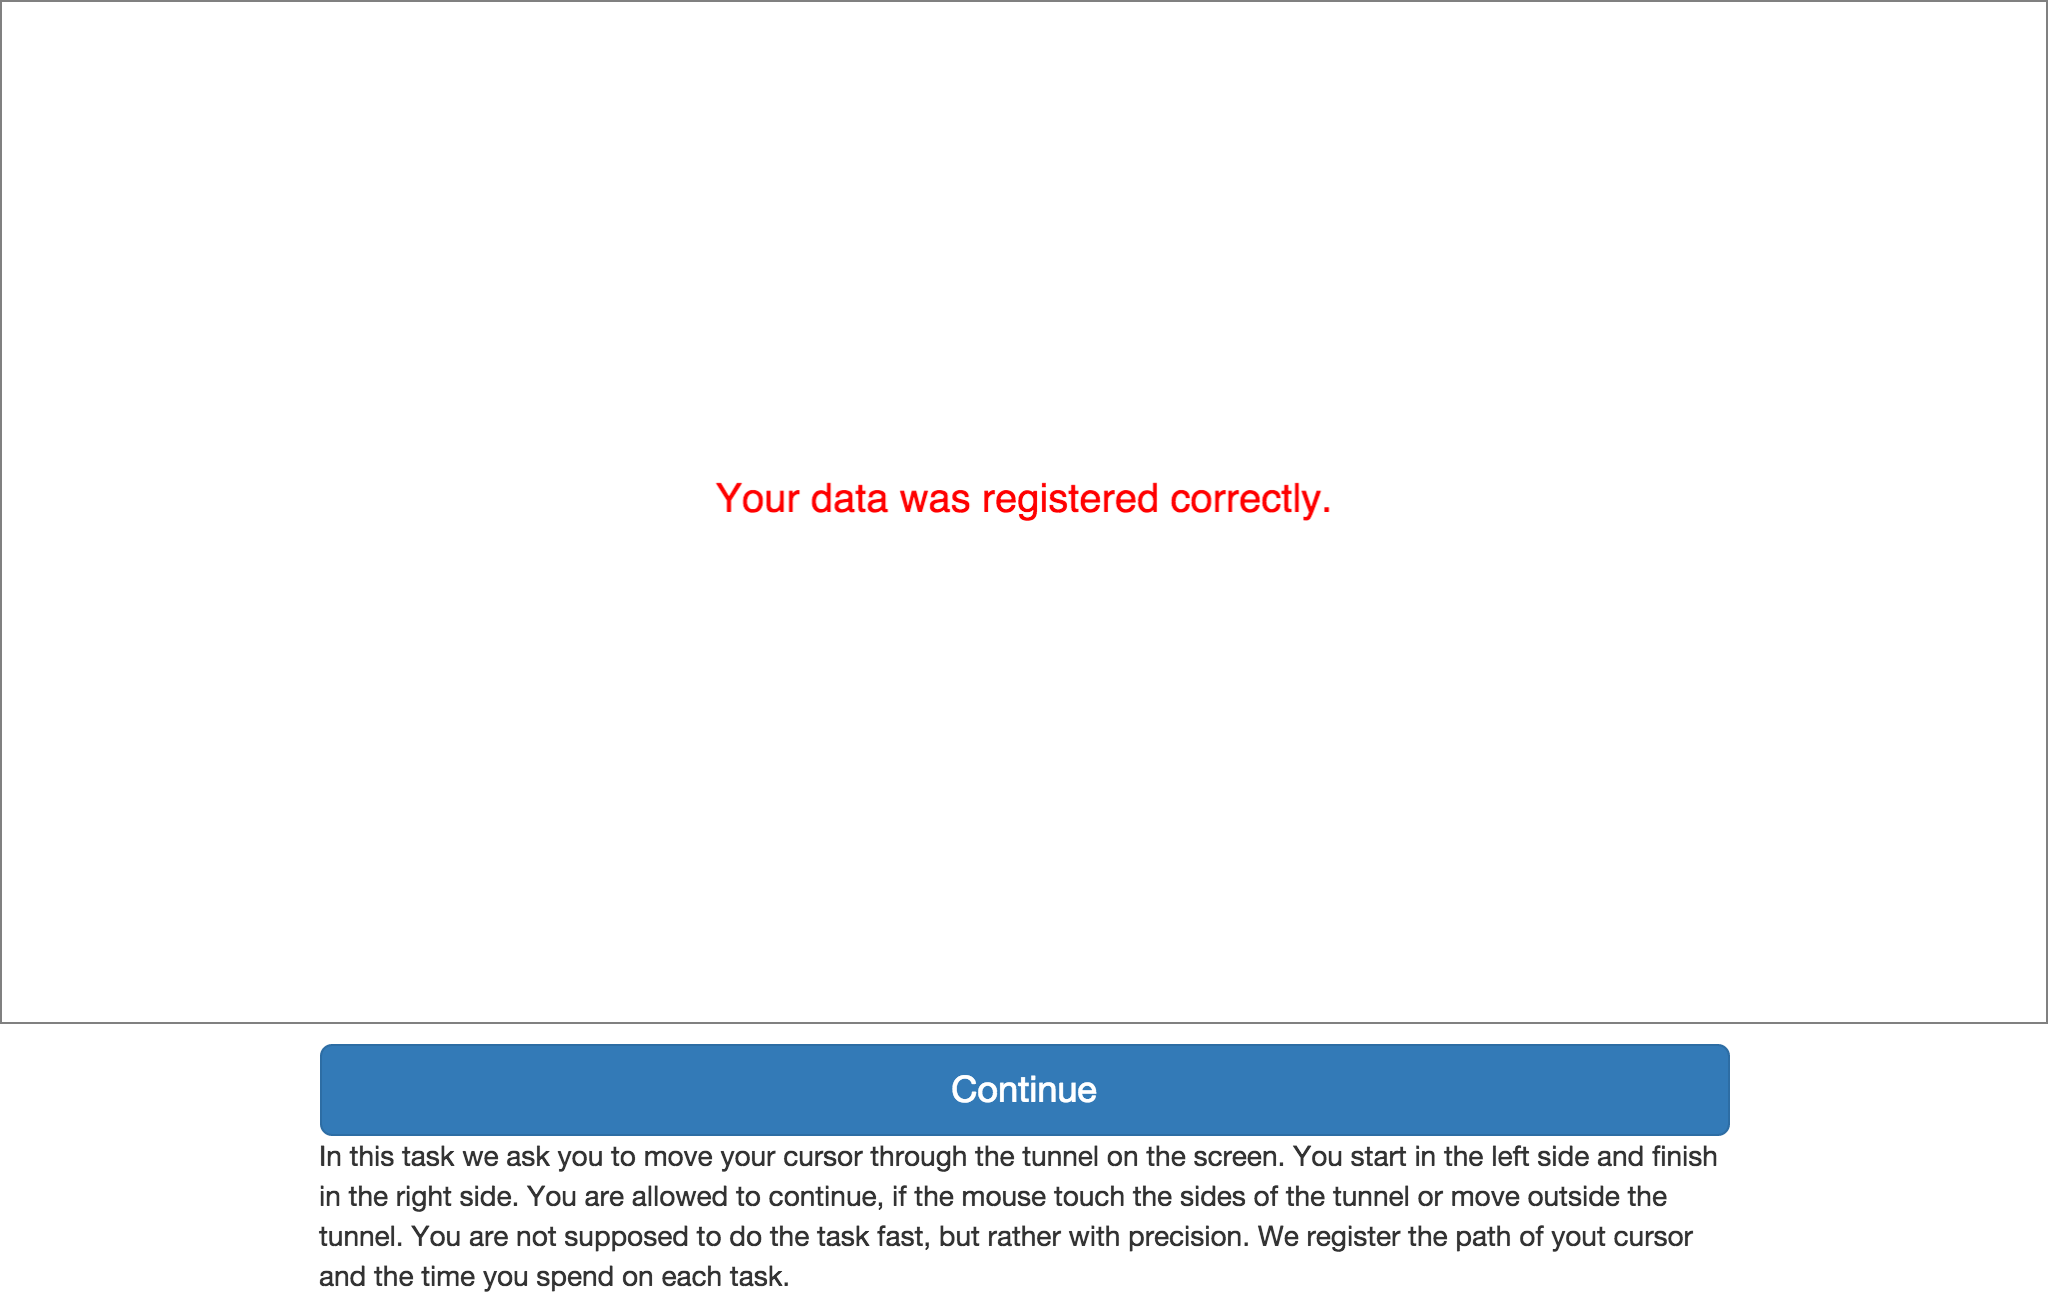
\includegraphics[width=\textwidth]{images/screenshots/ex_step_4_tunnel_done}
\captionof{figure}{Eksperiment - Trin 4 - Fortsæt}
\label{fig:ex_step_4_tunnel_done}
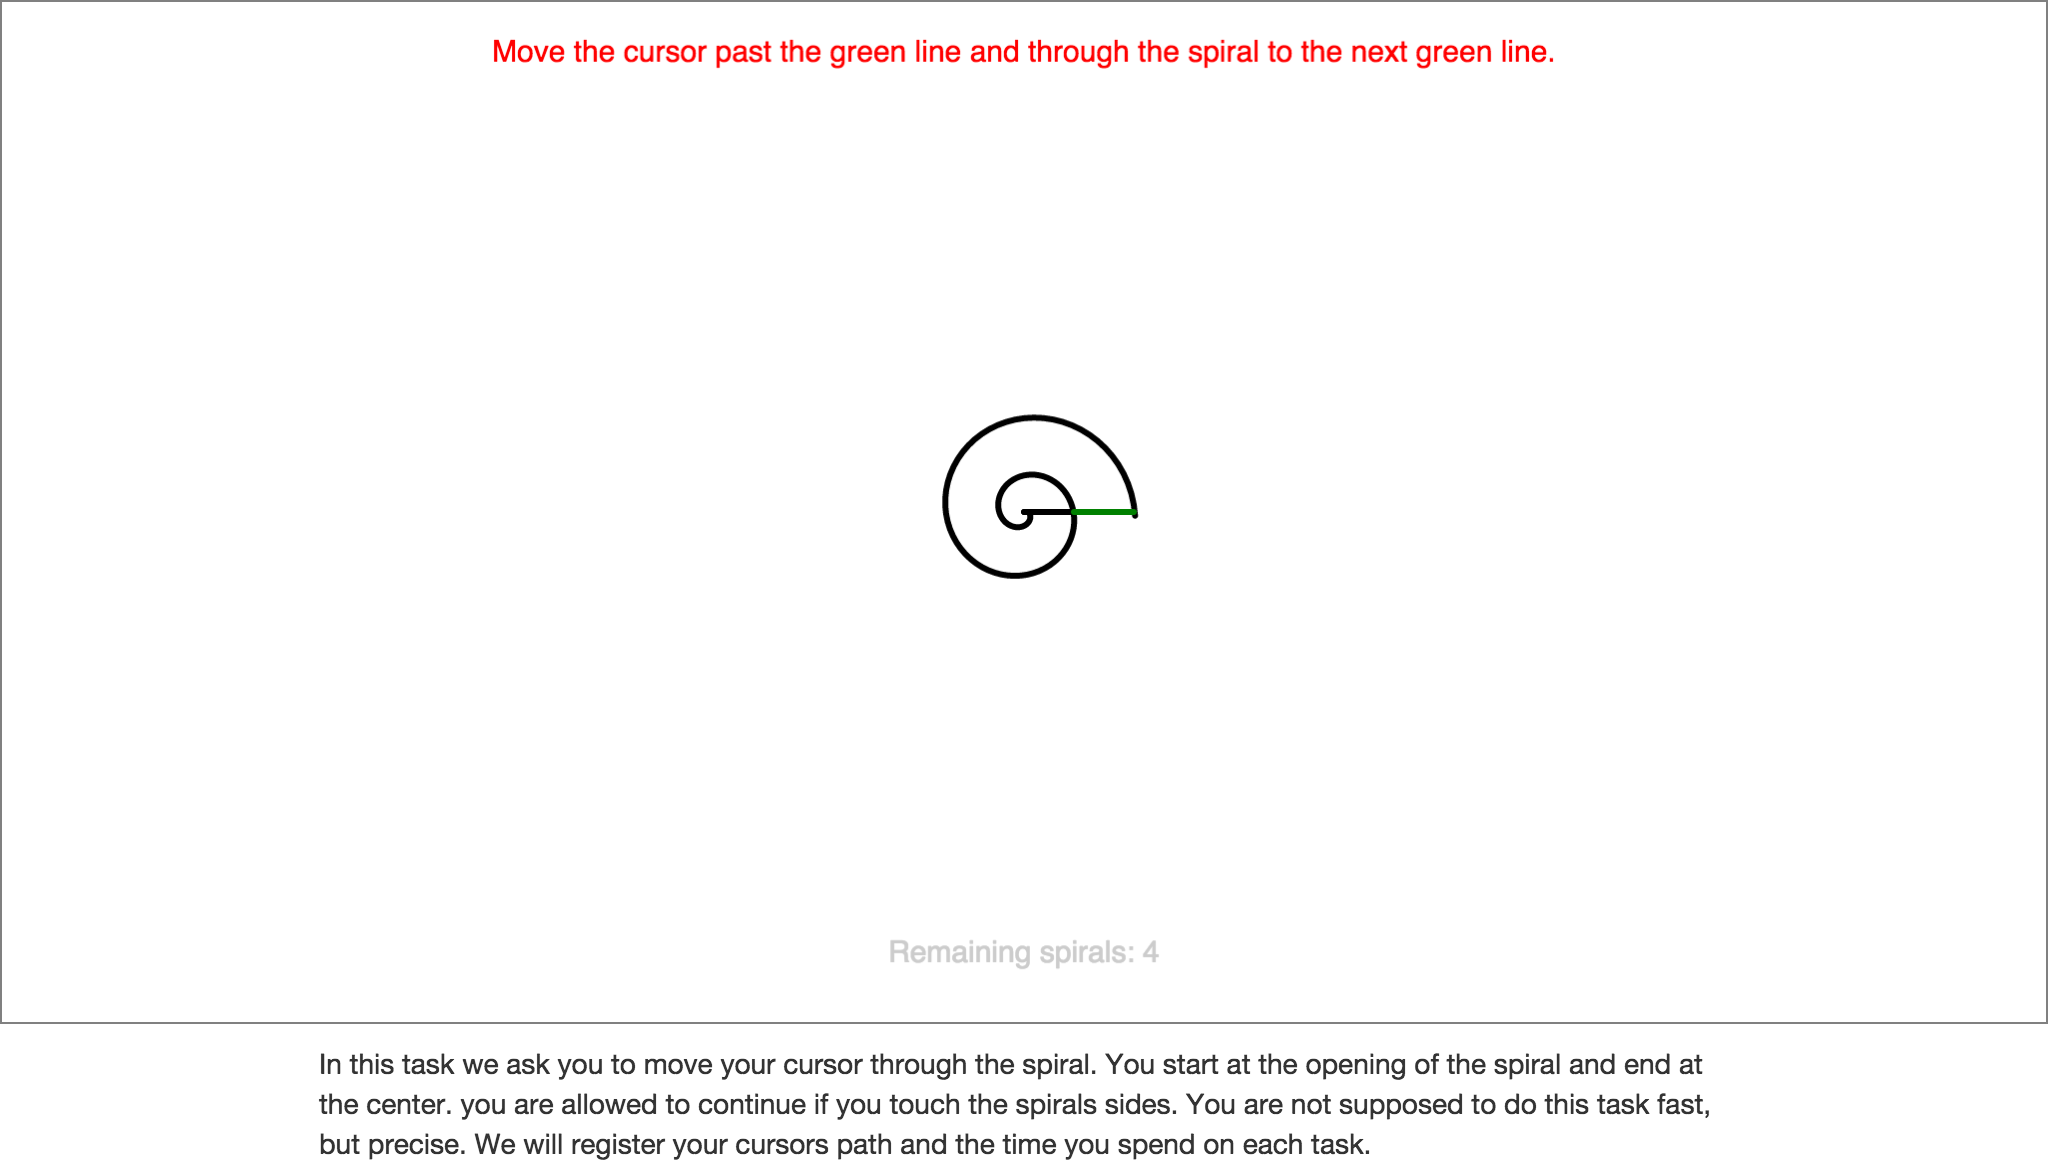
\includegraphics[width=\textwidth]{images/screenshots/ex_step_5_spiral_1}
\captionof{figure}{Eksperiment - Trin 5 - Spiral 1}
\label{fig:ex_step_5_spiral_1}
\end{minipage}

\begin{minipage}{\textwidth}
\centering
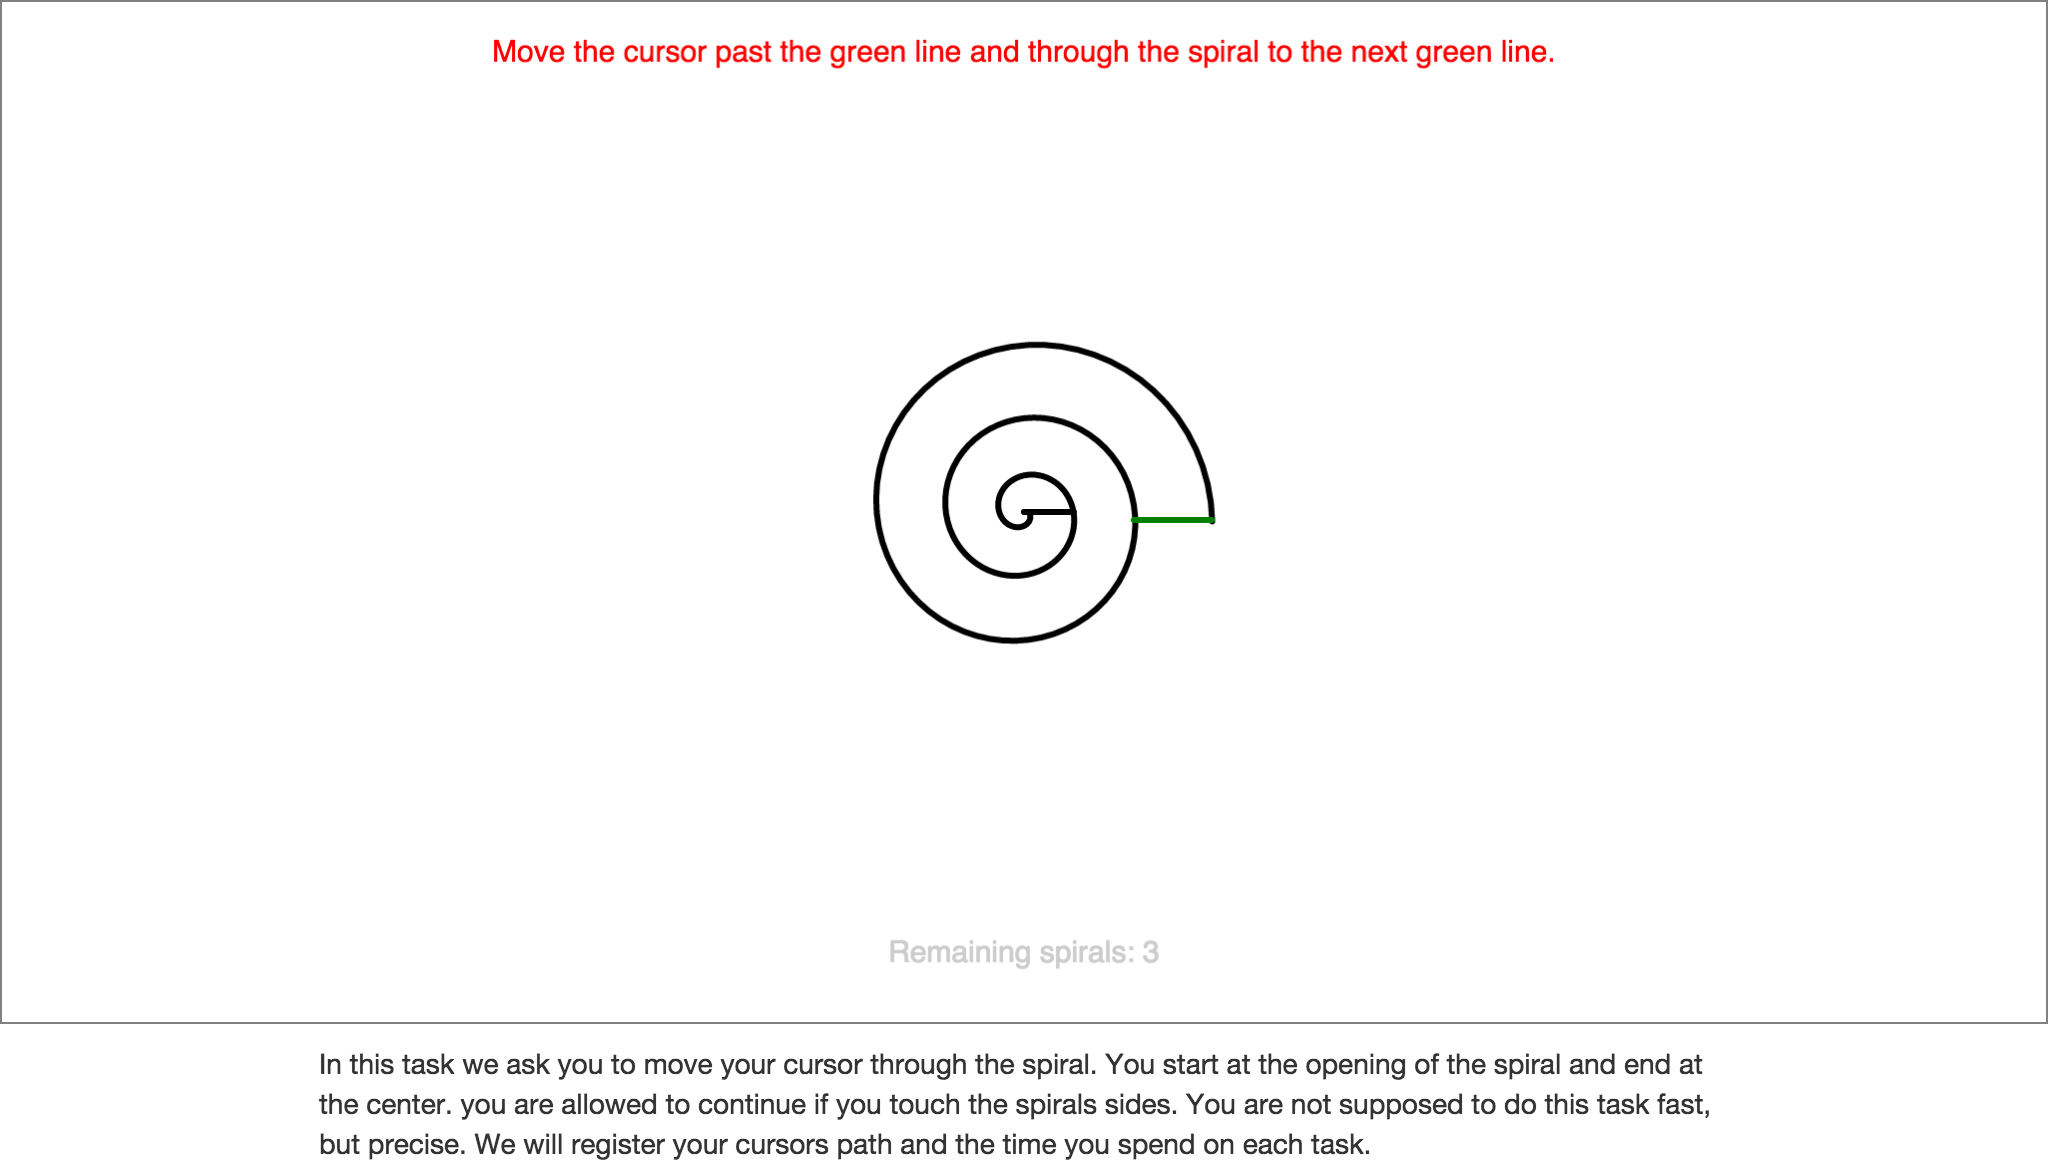
\includegraphics[width=\textwidth]{images/screenshots/ex_step_5_spiral_2}
\captionof{figure}{Eksperiment - Trin 5 - Spiral 2}
\label{fig:ex_step_5_spiral_2}
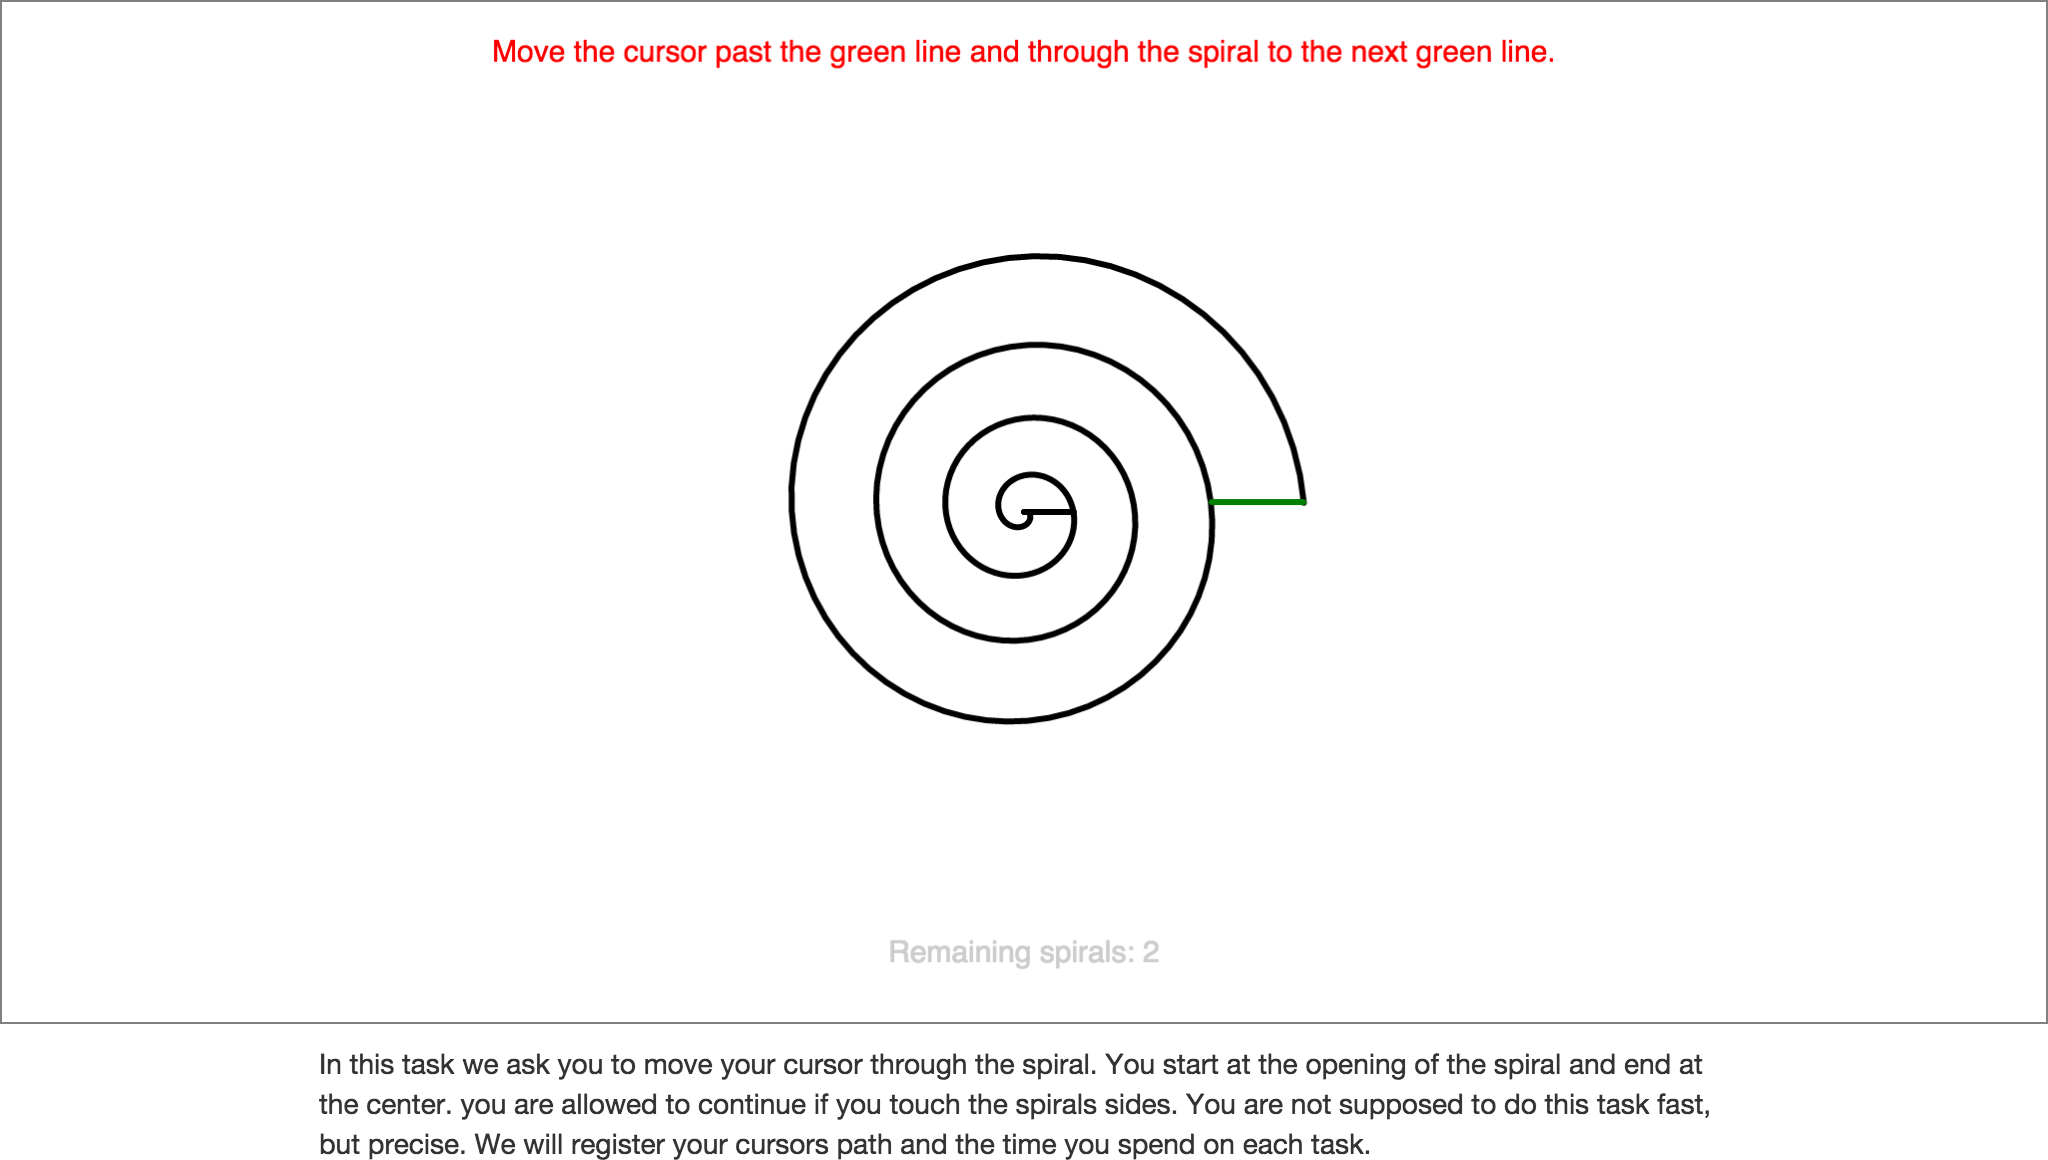
\includegraphics[width=\textwidth]{images/screenshots/ex_step_5_spiral_3}
\captionof{figure}{Eksperiment - Trin 5 - Spiral 3}
\label{fig:ex_step_5_spiral_3}
\end{minipage}

\begin{minipage}{\textwidth}
\centering
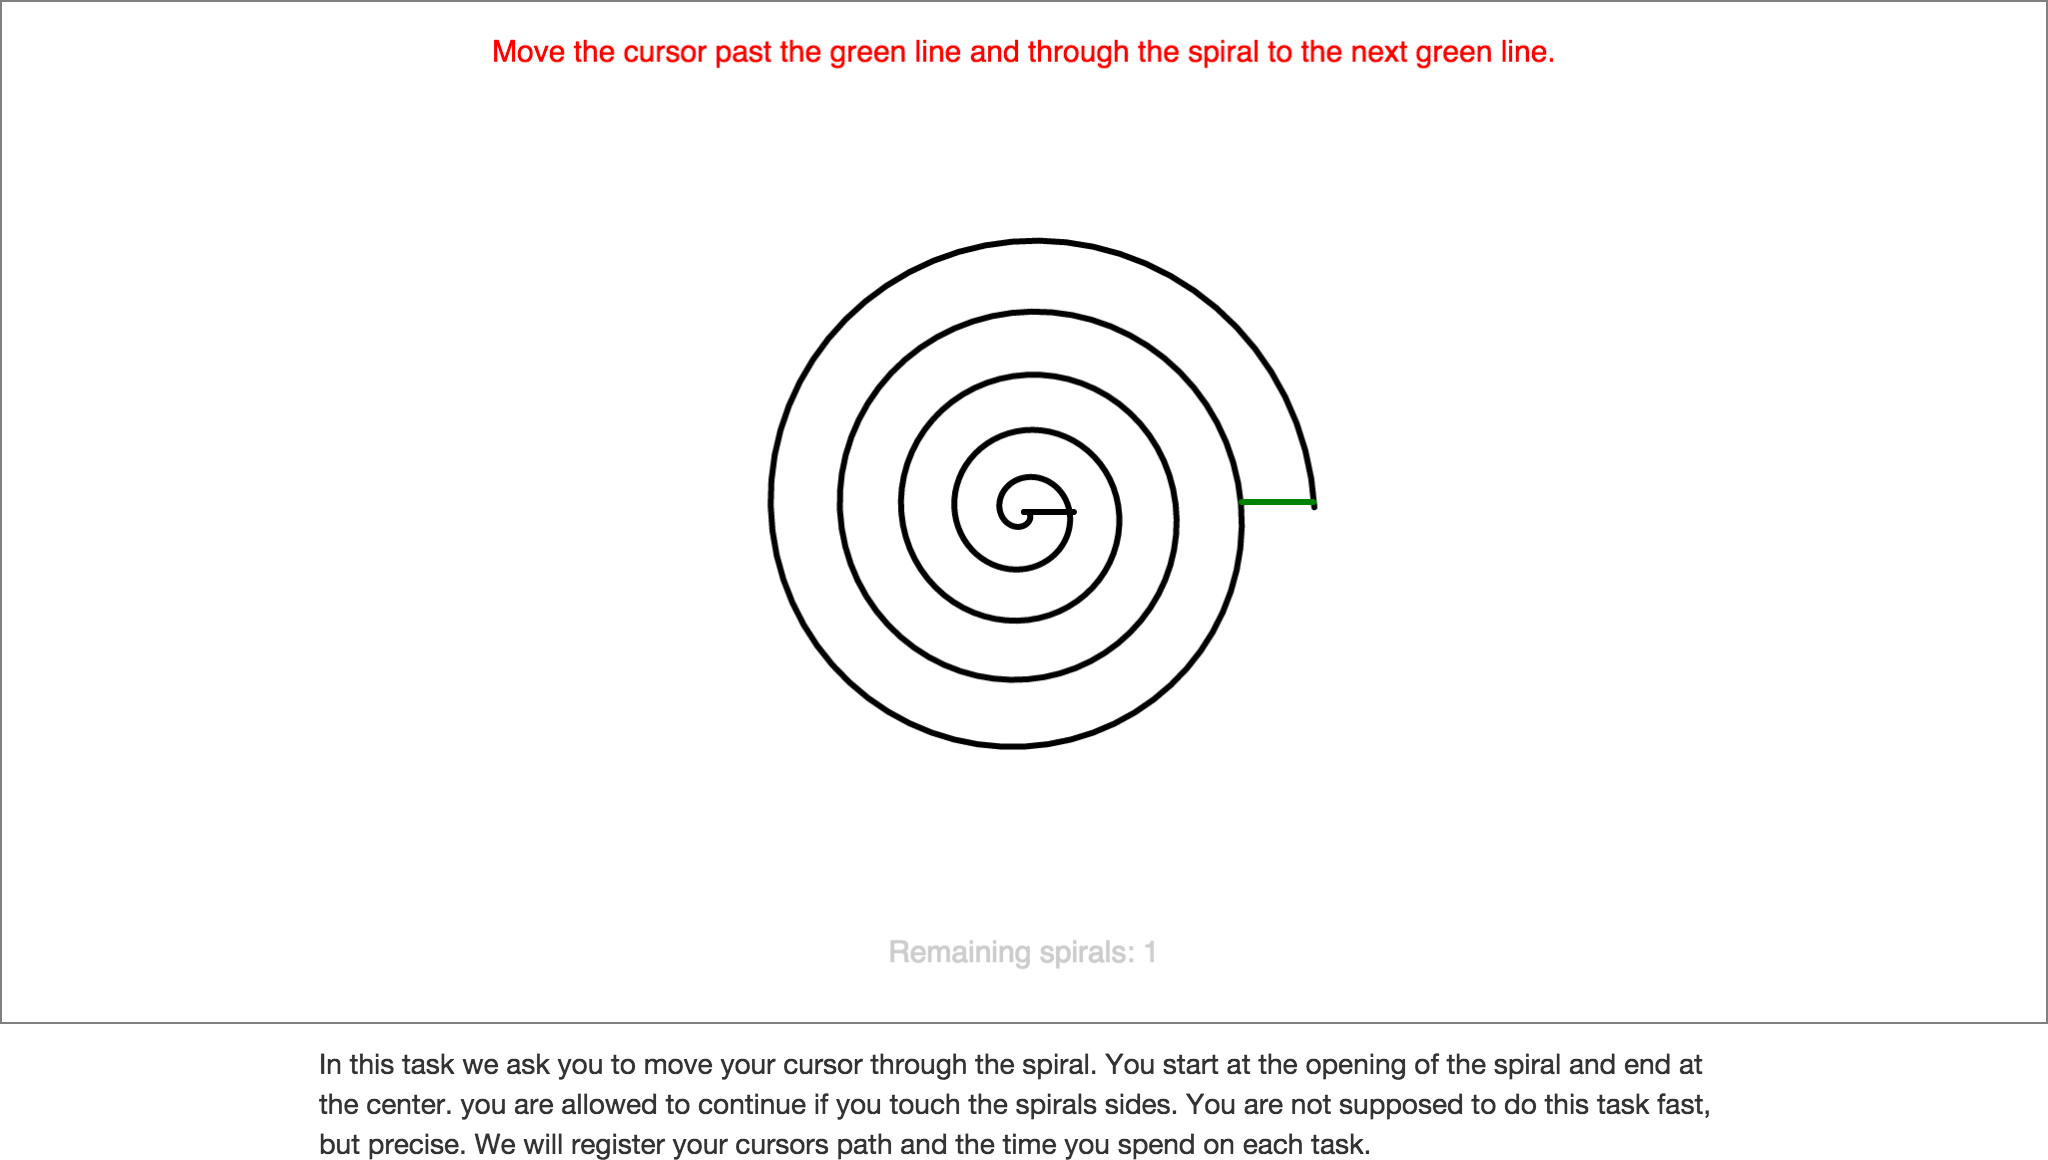
\includegraphics[width=\textwidth]{images/screenshots/ex_step_5_spiral_4}
\captionof{figure}{Eksperiment - Trin 5 - Spiral 4}
\label{fig:ex_step_5_spiral_4}
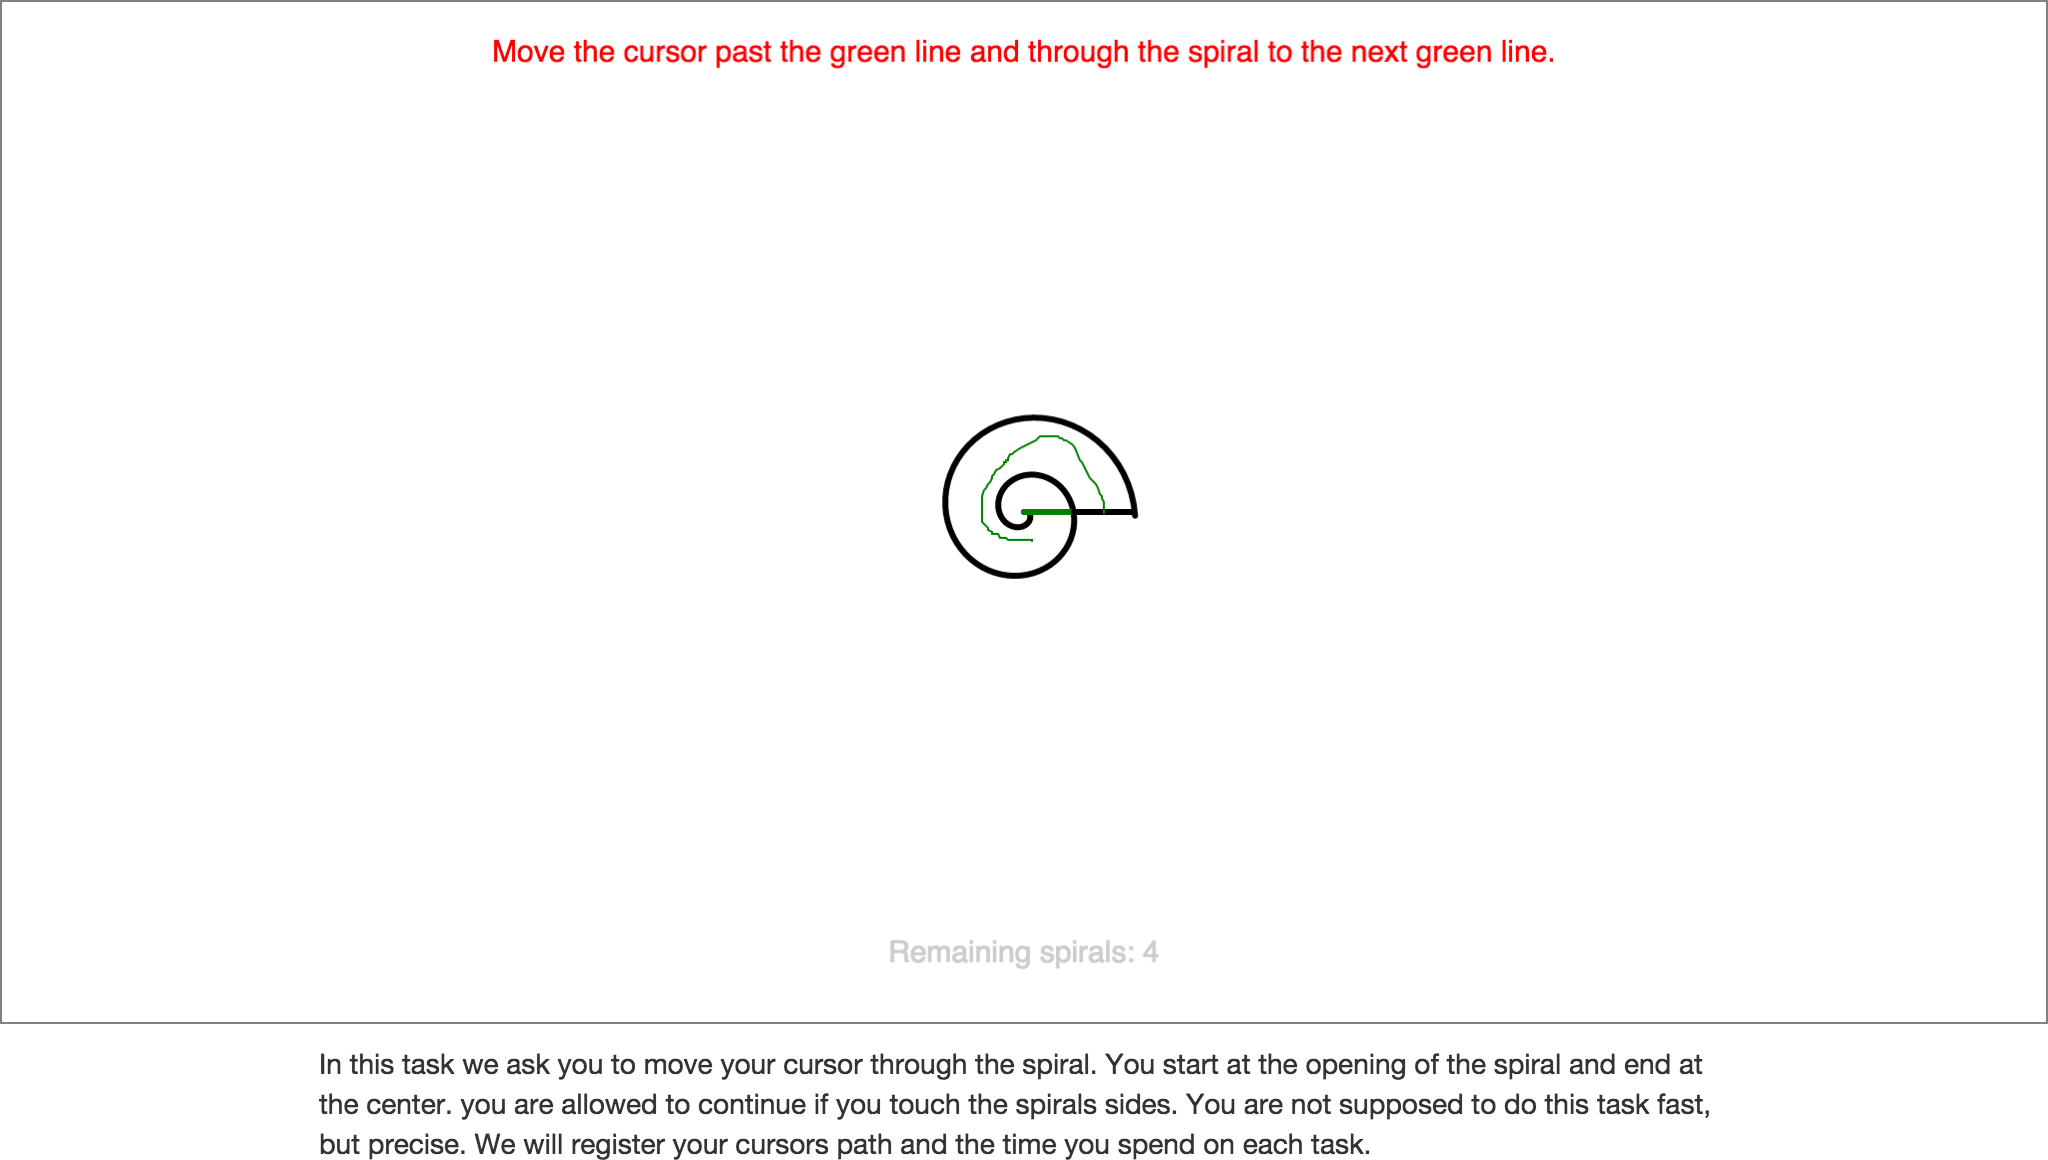
\includegraphics[width=\textwidth]{images/screenshots/ex_step_5_spiral_path}
\captionof{figure}{Eksperiment - Trin 5 - Spiralbane}
\label{fig:ex_step_5_spiral_path}
\end{minipage}

\begin{minipage}{\textwidth}
\centering
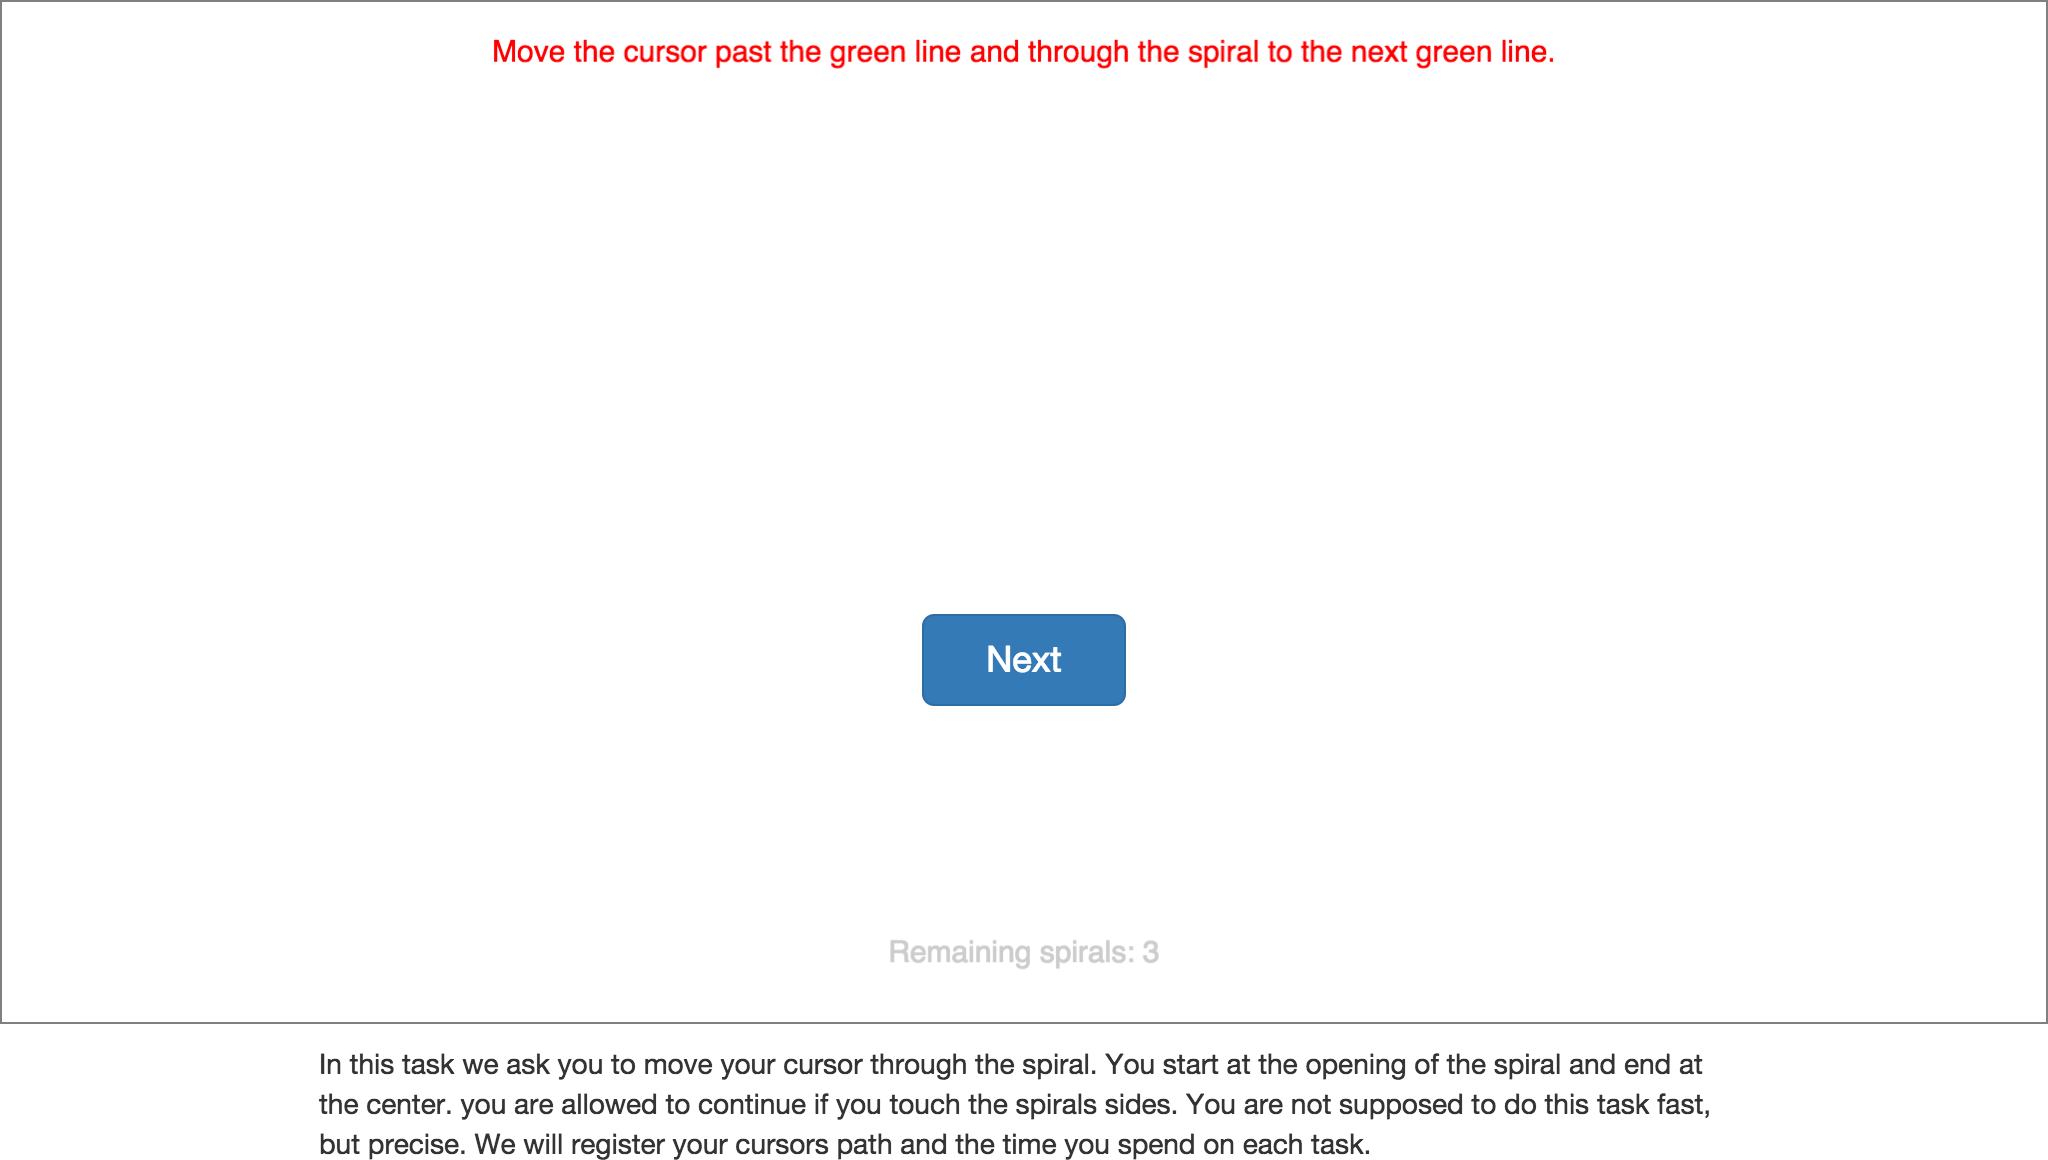
\includegraphics[width=\textwidth]{images/screenshots/ex_step_5_spiral_next}
\captionof{figure}{Eksperiment - Trin 5 - Næste spiral}
\label{fig:ex_step_5_spiral_next}
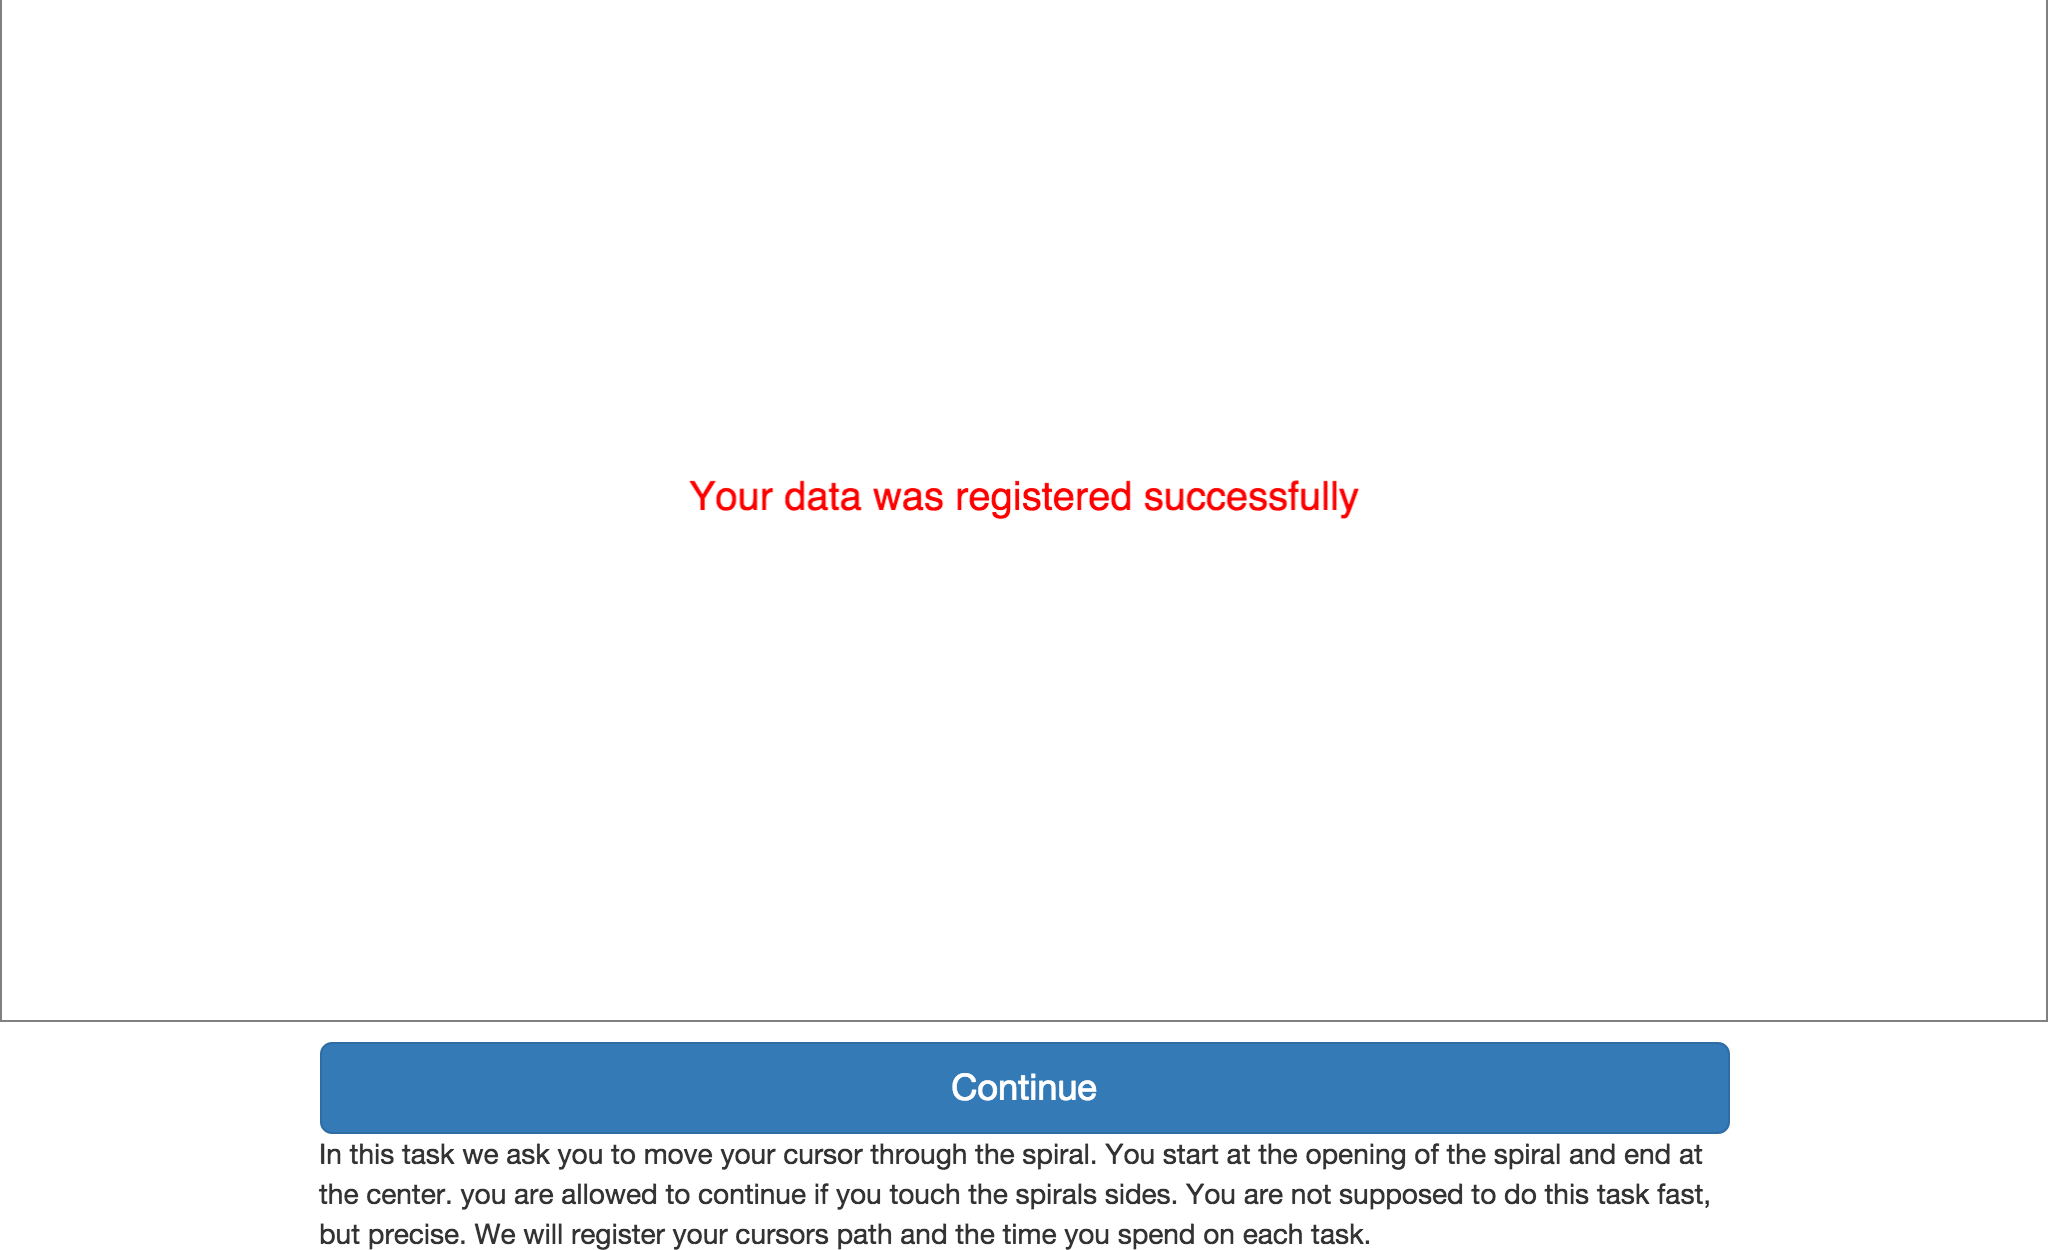
\includegraphics[width=\textwidth]{images/screenshots/ex_step_5_spiral_done}
\captionof{figure}{Eksperiment - Trin 5 - Fortsæt}
\label{fig:ex_step_5_spiral_done}
\end{minipage}

\begin{minipage}{\textwidth}
\centering
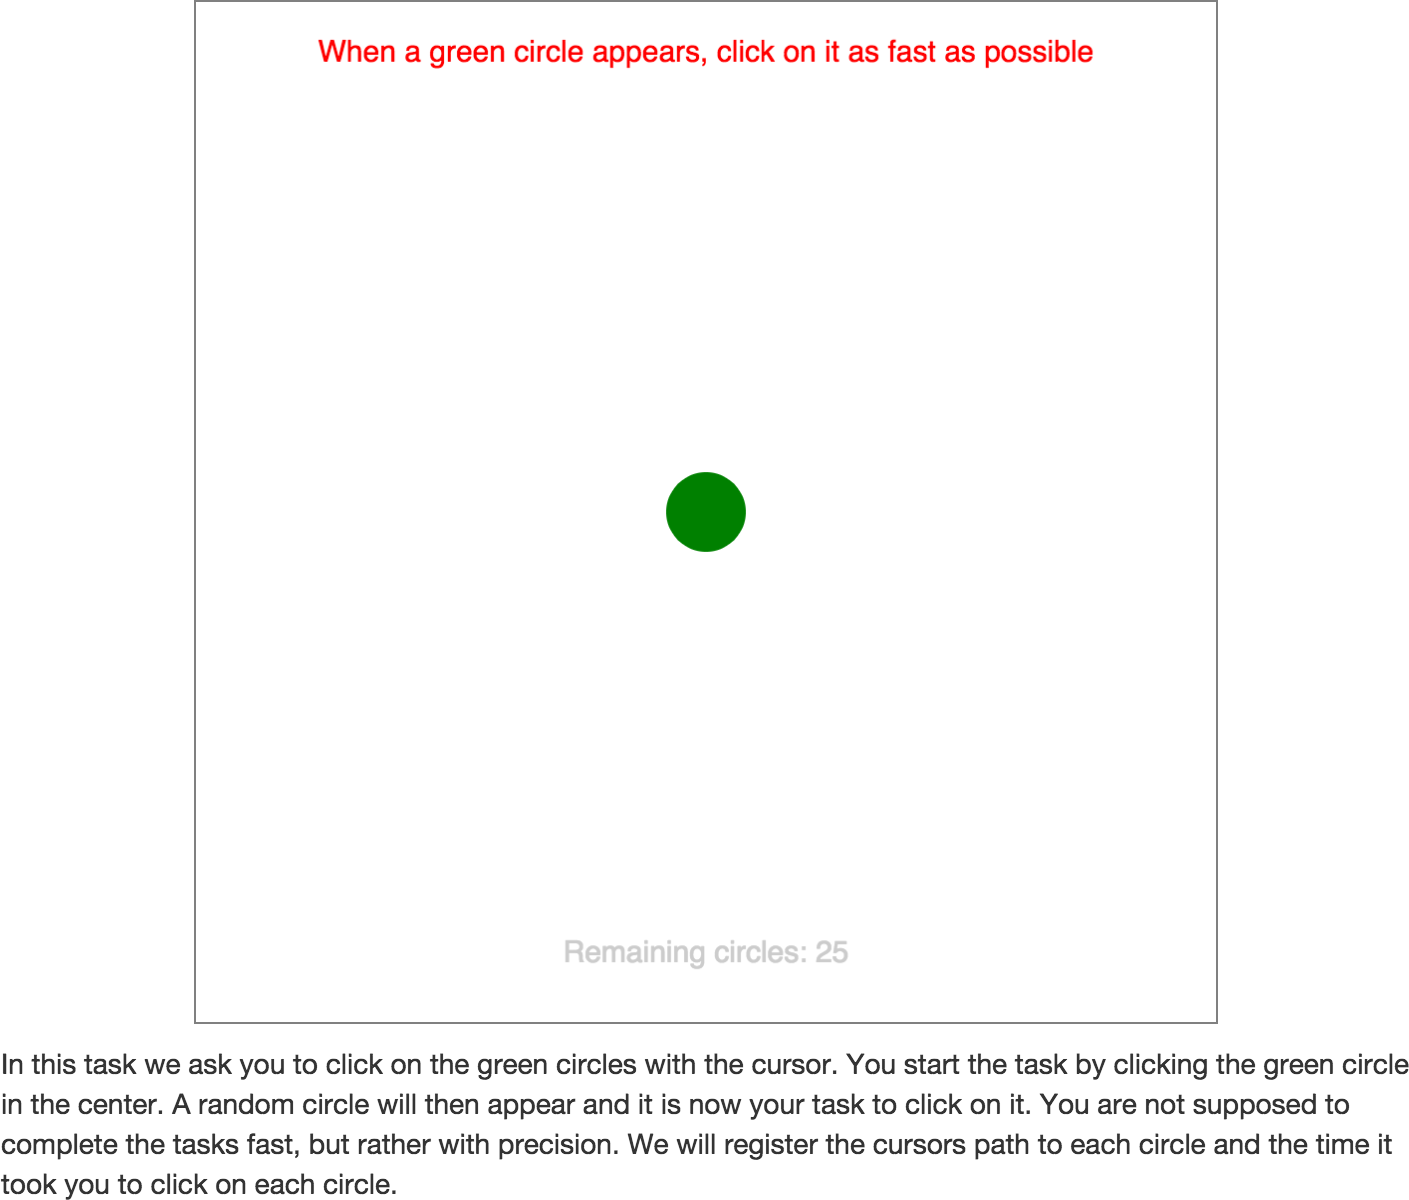
\includegraphics[height=.4\textheight]{images/screenshots/ex_step_6_pointing_start}
\captionof{figure}{Eksperiment - Trin 6 - Start}
\label{fig:ex_step_6_pointing_start}
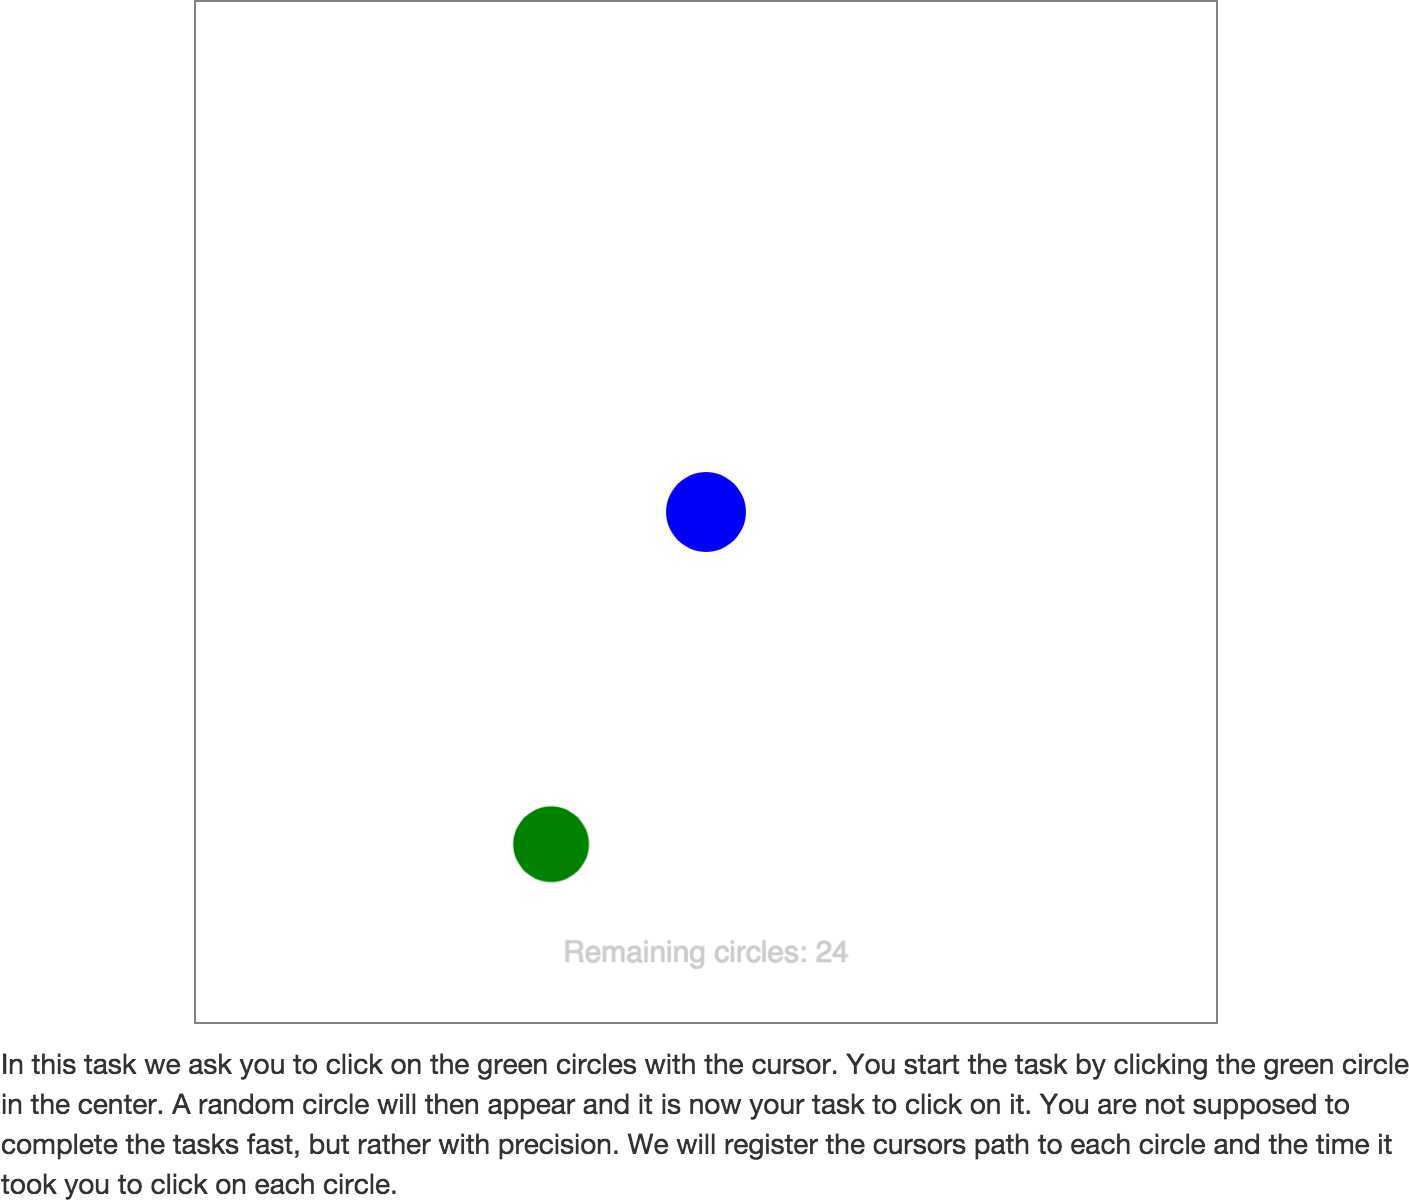
\includegraphics[height=.4\textheight]{images/screenshots/ex_step_6_pointing_target_1}
\captionof{figure}{Eksperiment - Trin 6 - Pegeeksempel 1}
\label{fig:ex_step_6_pointing_target_1}
\end{minipage}

\begin{minipage}{\textwidth}
\centering
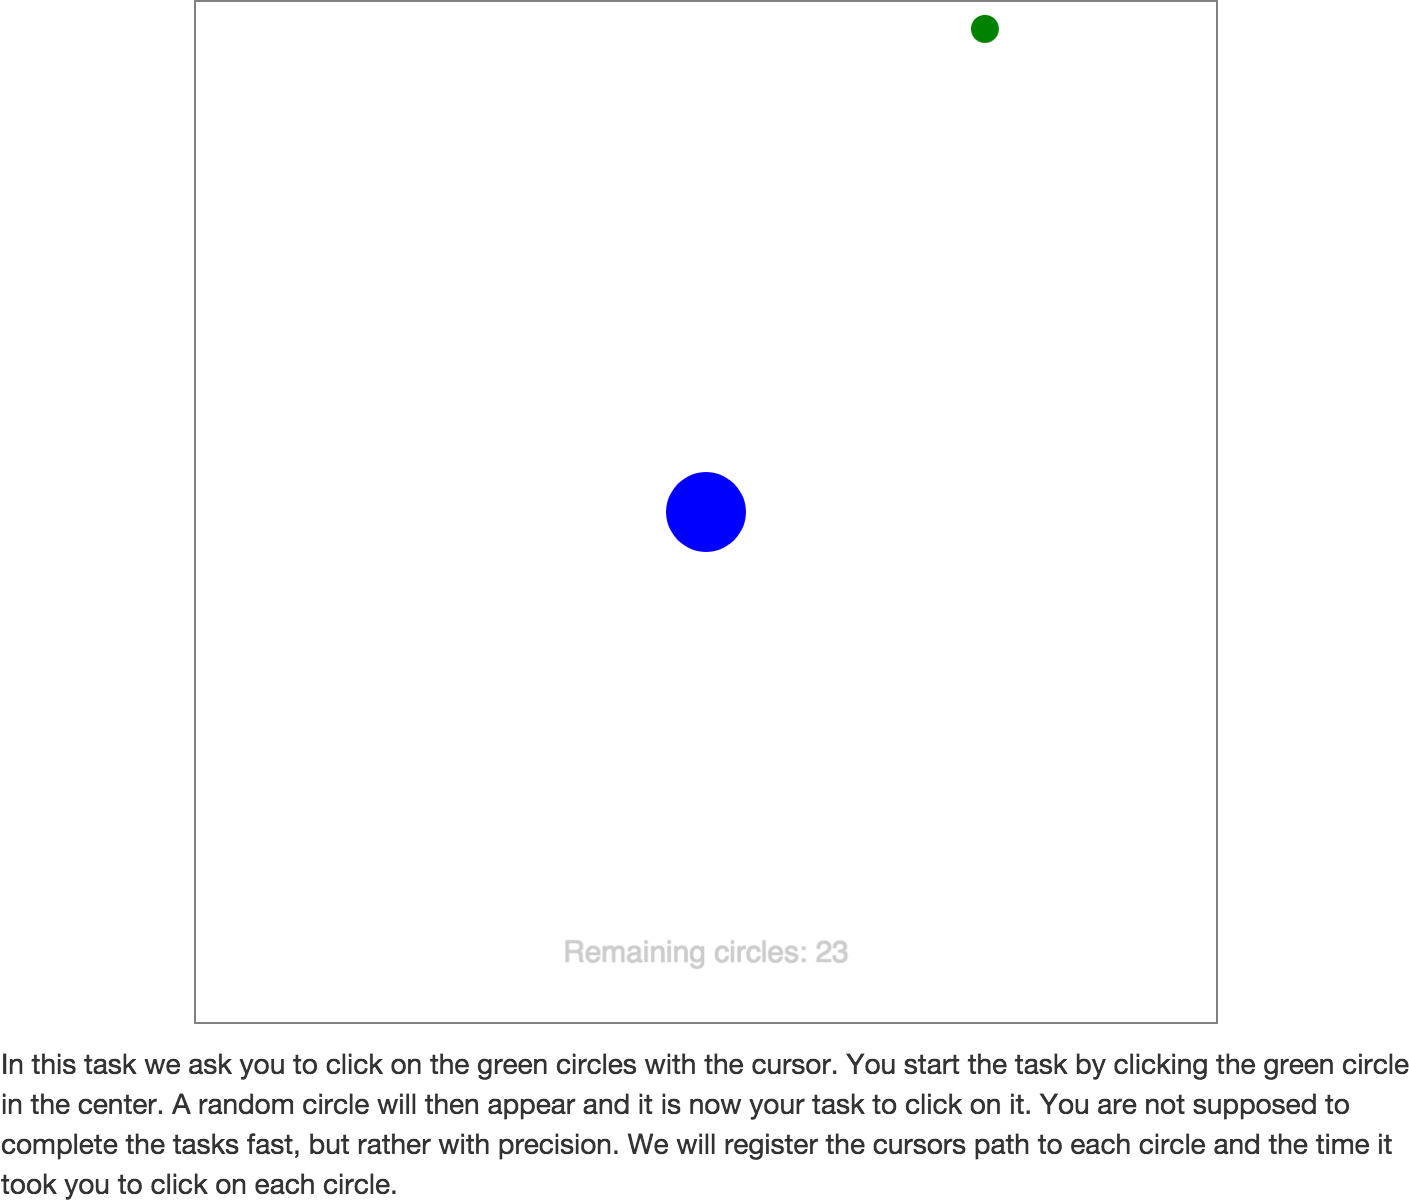
\includegraphics[height=.4\textheight]{images/screenshots/ex_step_6_pointing_target_2}
\captionof{figure}{Eksperiment - Trin 6 - Pegeeksempel 2}
\label{fig:ex_step_6_pointing_target_2}
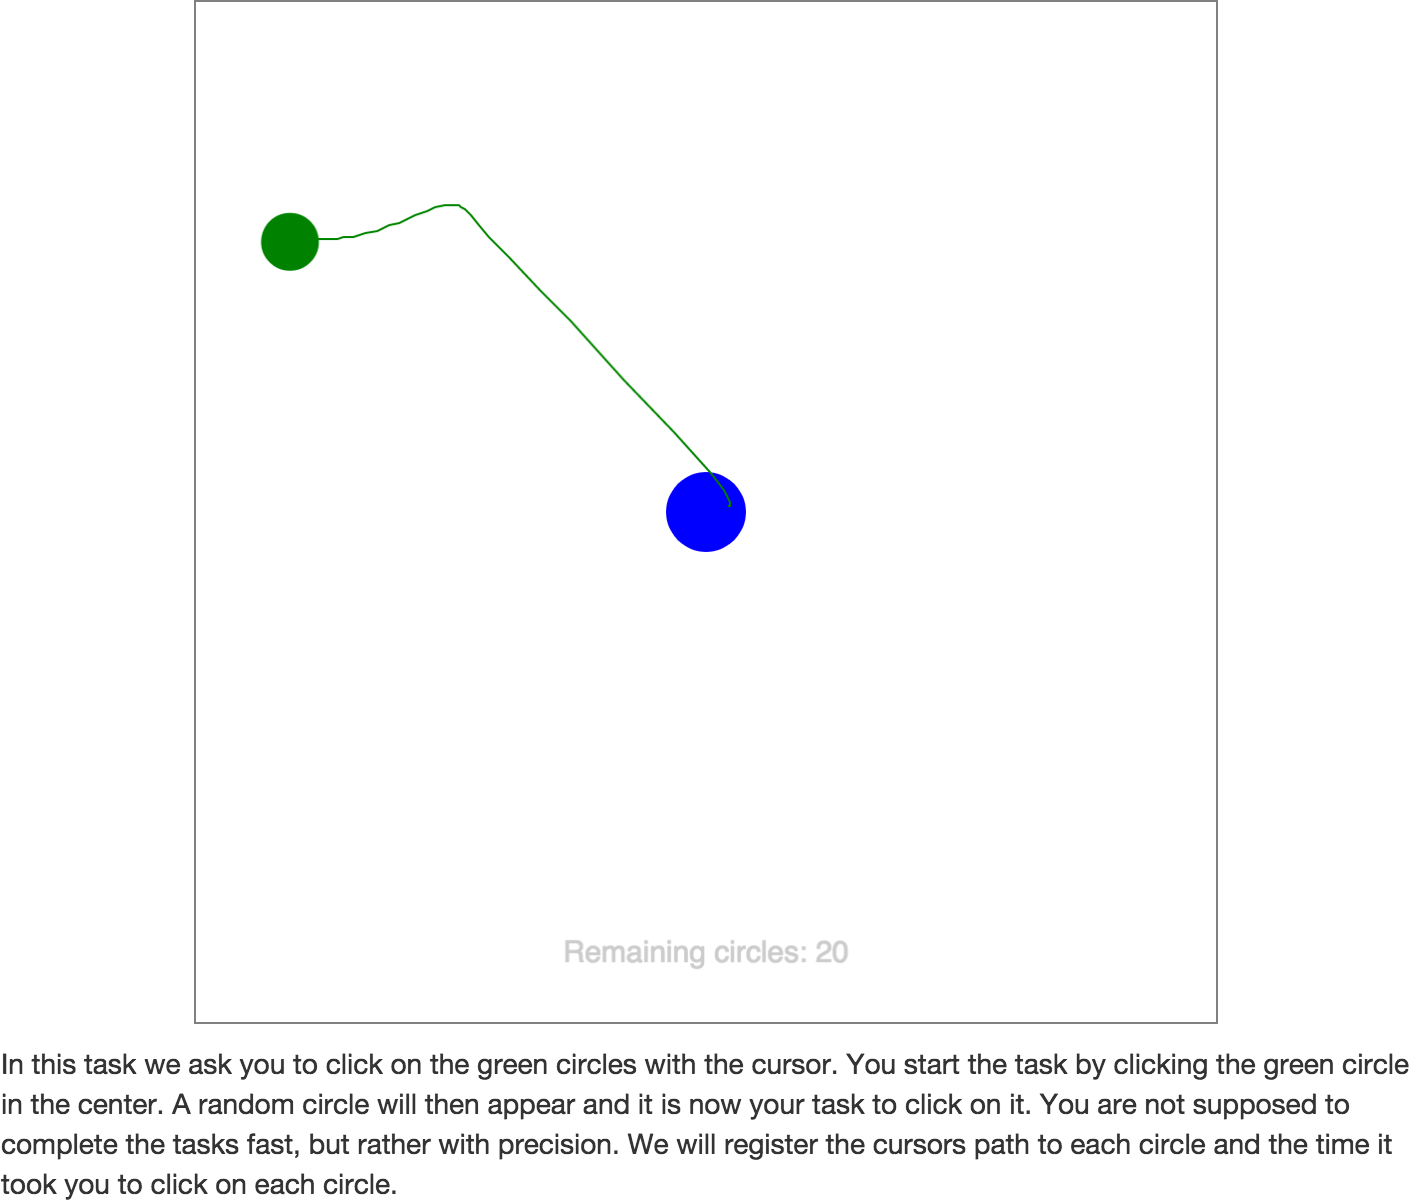
\includegraphics[height=.4\textheight]{images/screenshots/ex_step_6_pointing_path}
\captionof{figure}{Eksperiment - Trin 6 - Pegebane}
\label{fig:ex_step_6_pointing_path}
\end{minipage}

\begin{minipage}{\textwidth}
\centering
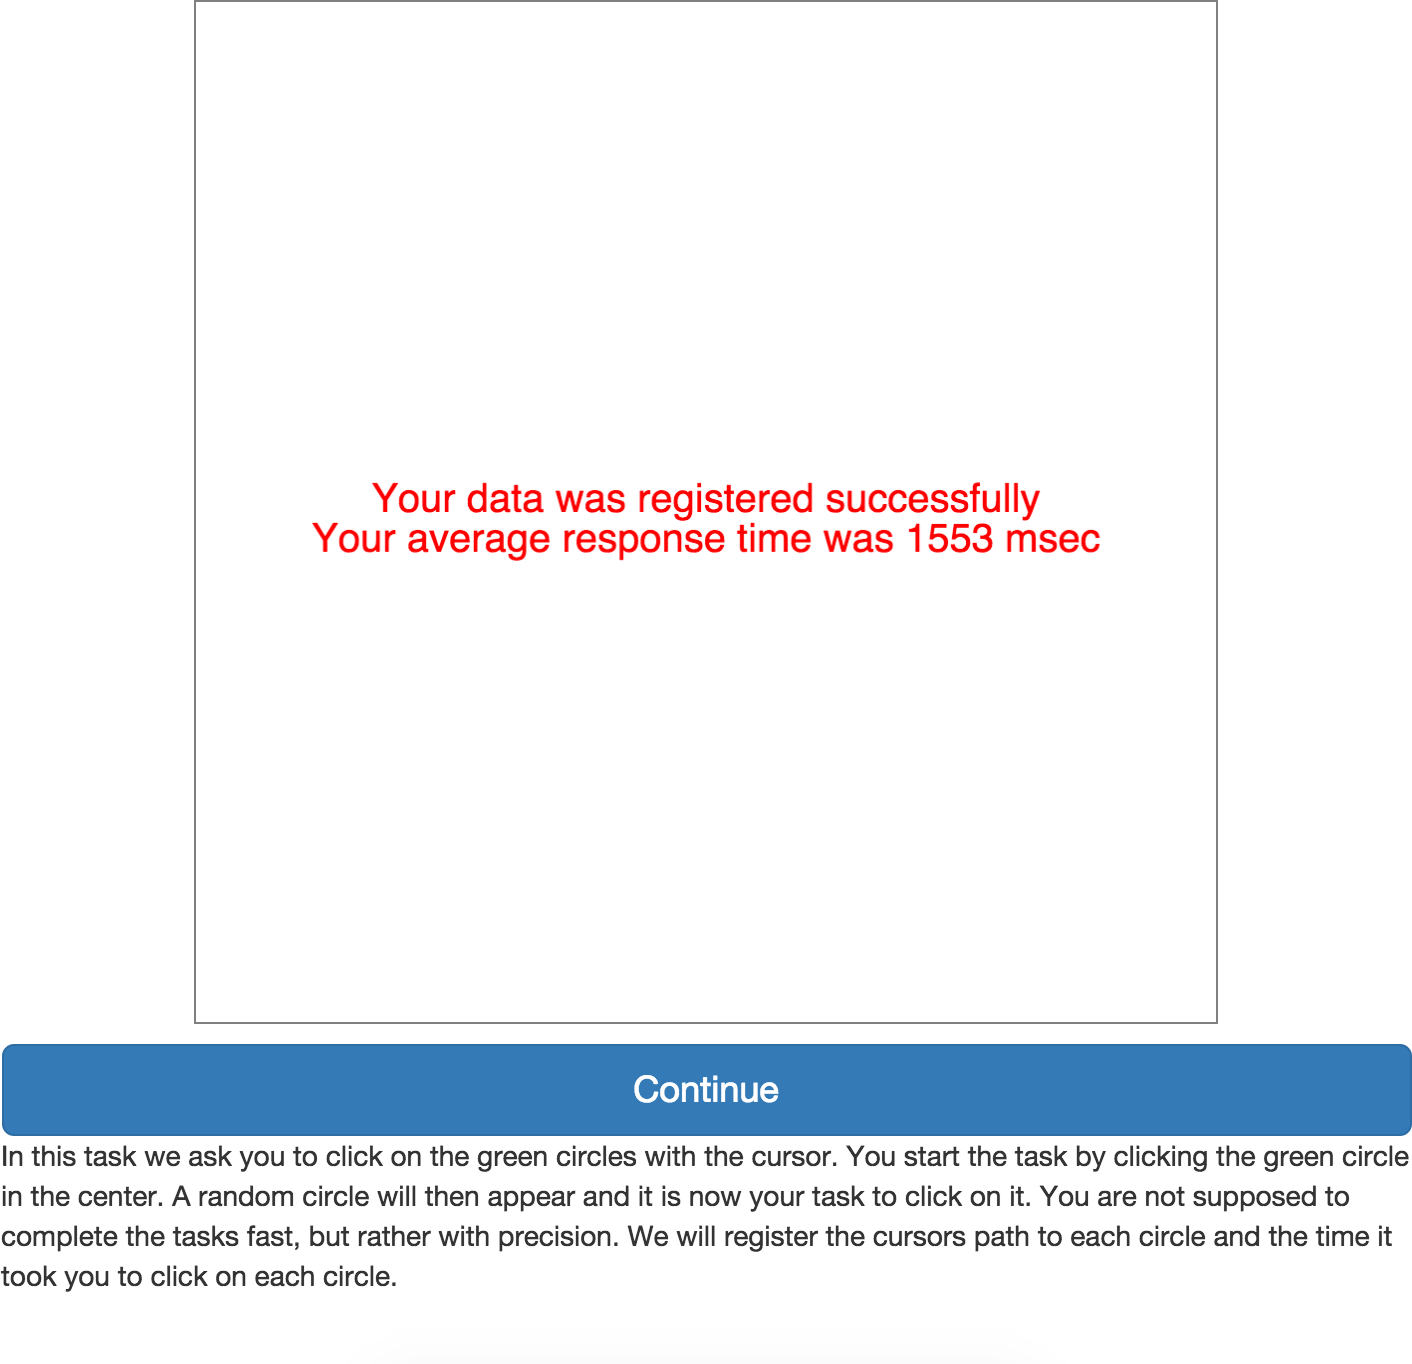
\includegraphics[height=.4\textheight]{images/screenshots/ex_step_6_pointing_done}
\captionof{figure}{Eksperiment - Trin 6 - Færdig}
\label{fig:ex_step_6_pointing_done}
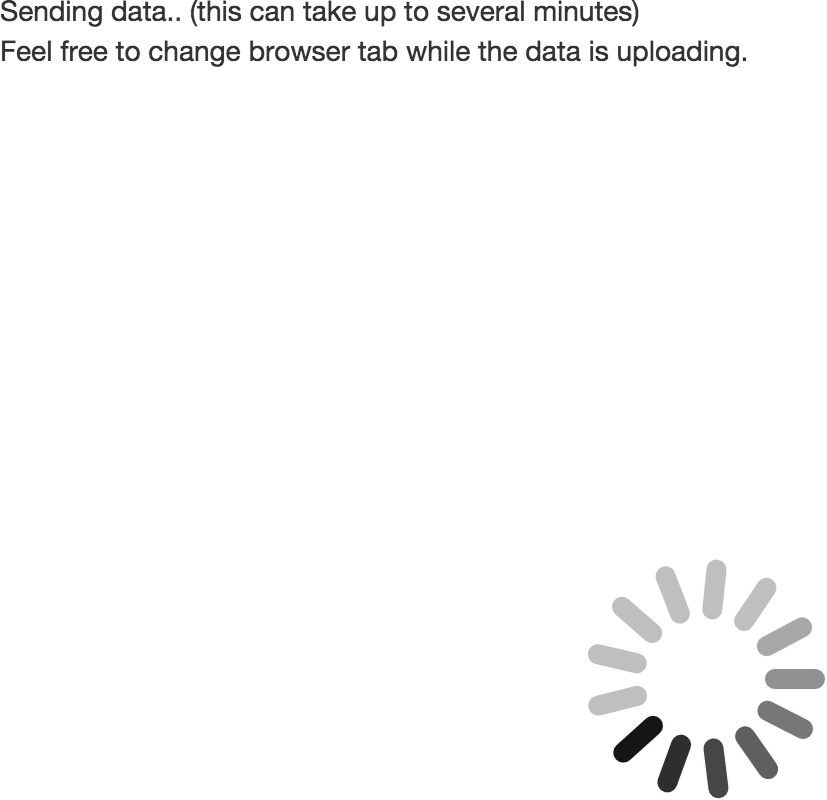
\includegraphics[height=.4\textheight]{images/screenshots/ex_step_7_sending}
\captionof{figure}{Eksperiment - Trin 7 - Sender}
\label{fig:ex_step_7_sending}
\end{minipage}

%-- Kvalitativ analyse --%
\newpage
\chapter{Testdeltageres bevægelsesbaner}
\label{sec:movementlines}
\begin{minipage}{\textwidth}
	\begin{minipage}{0.5\linewidth}
		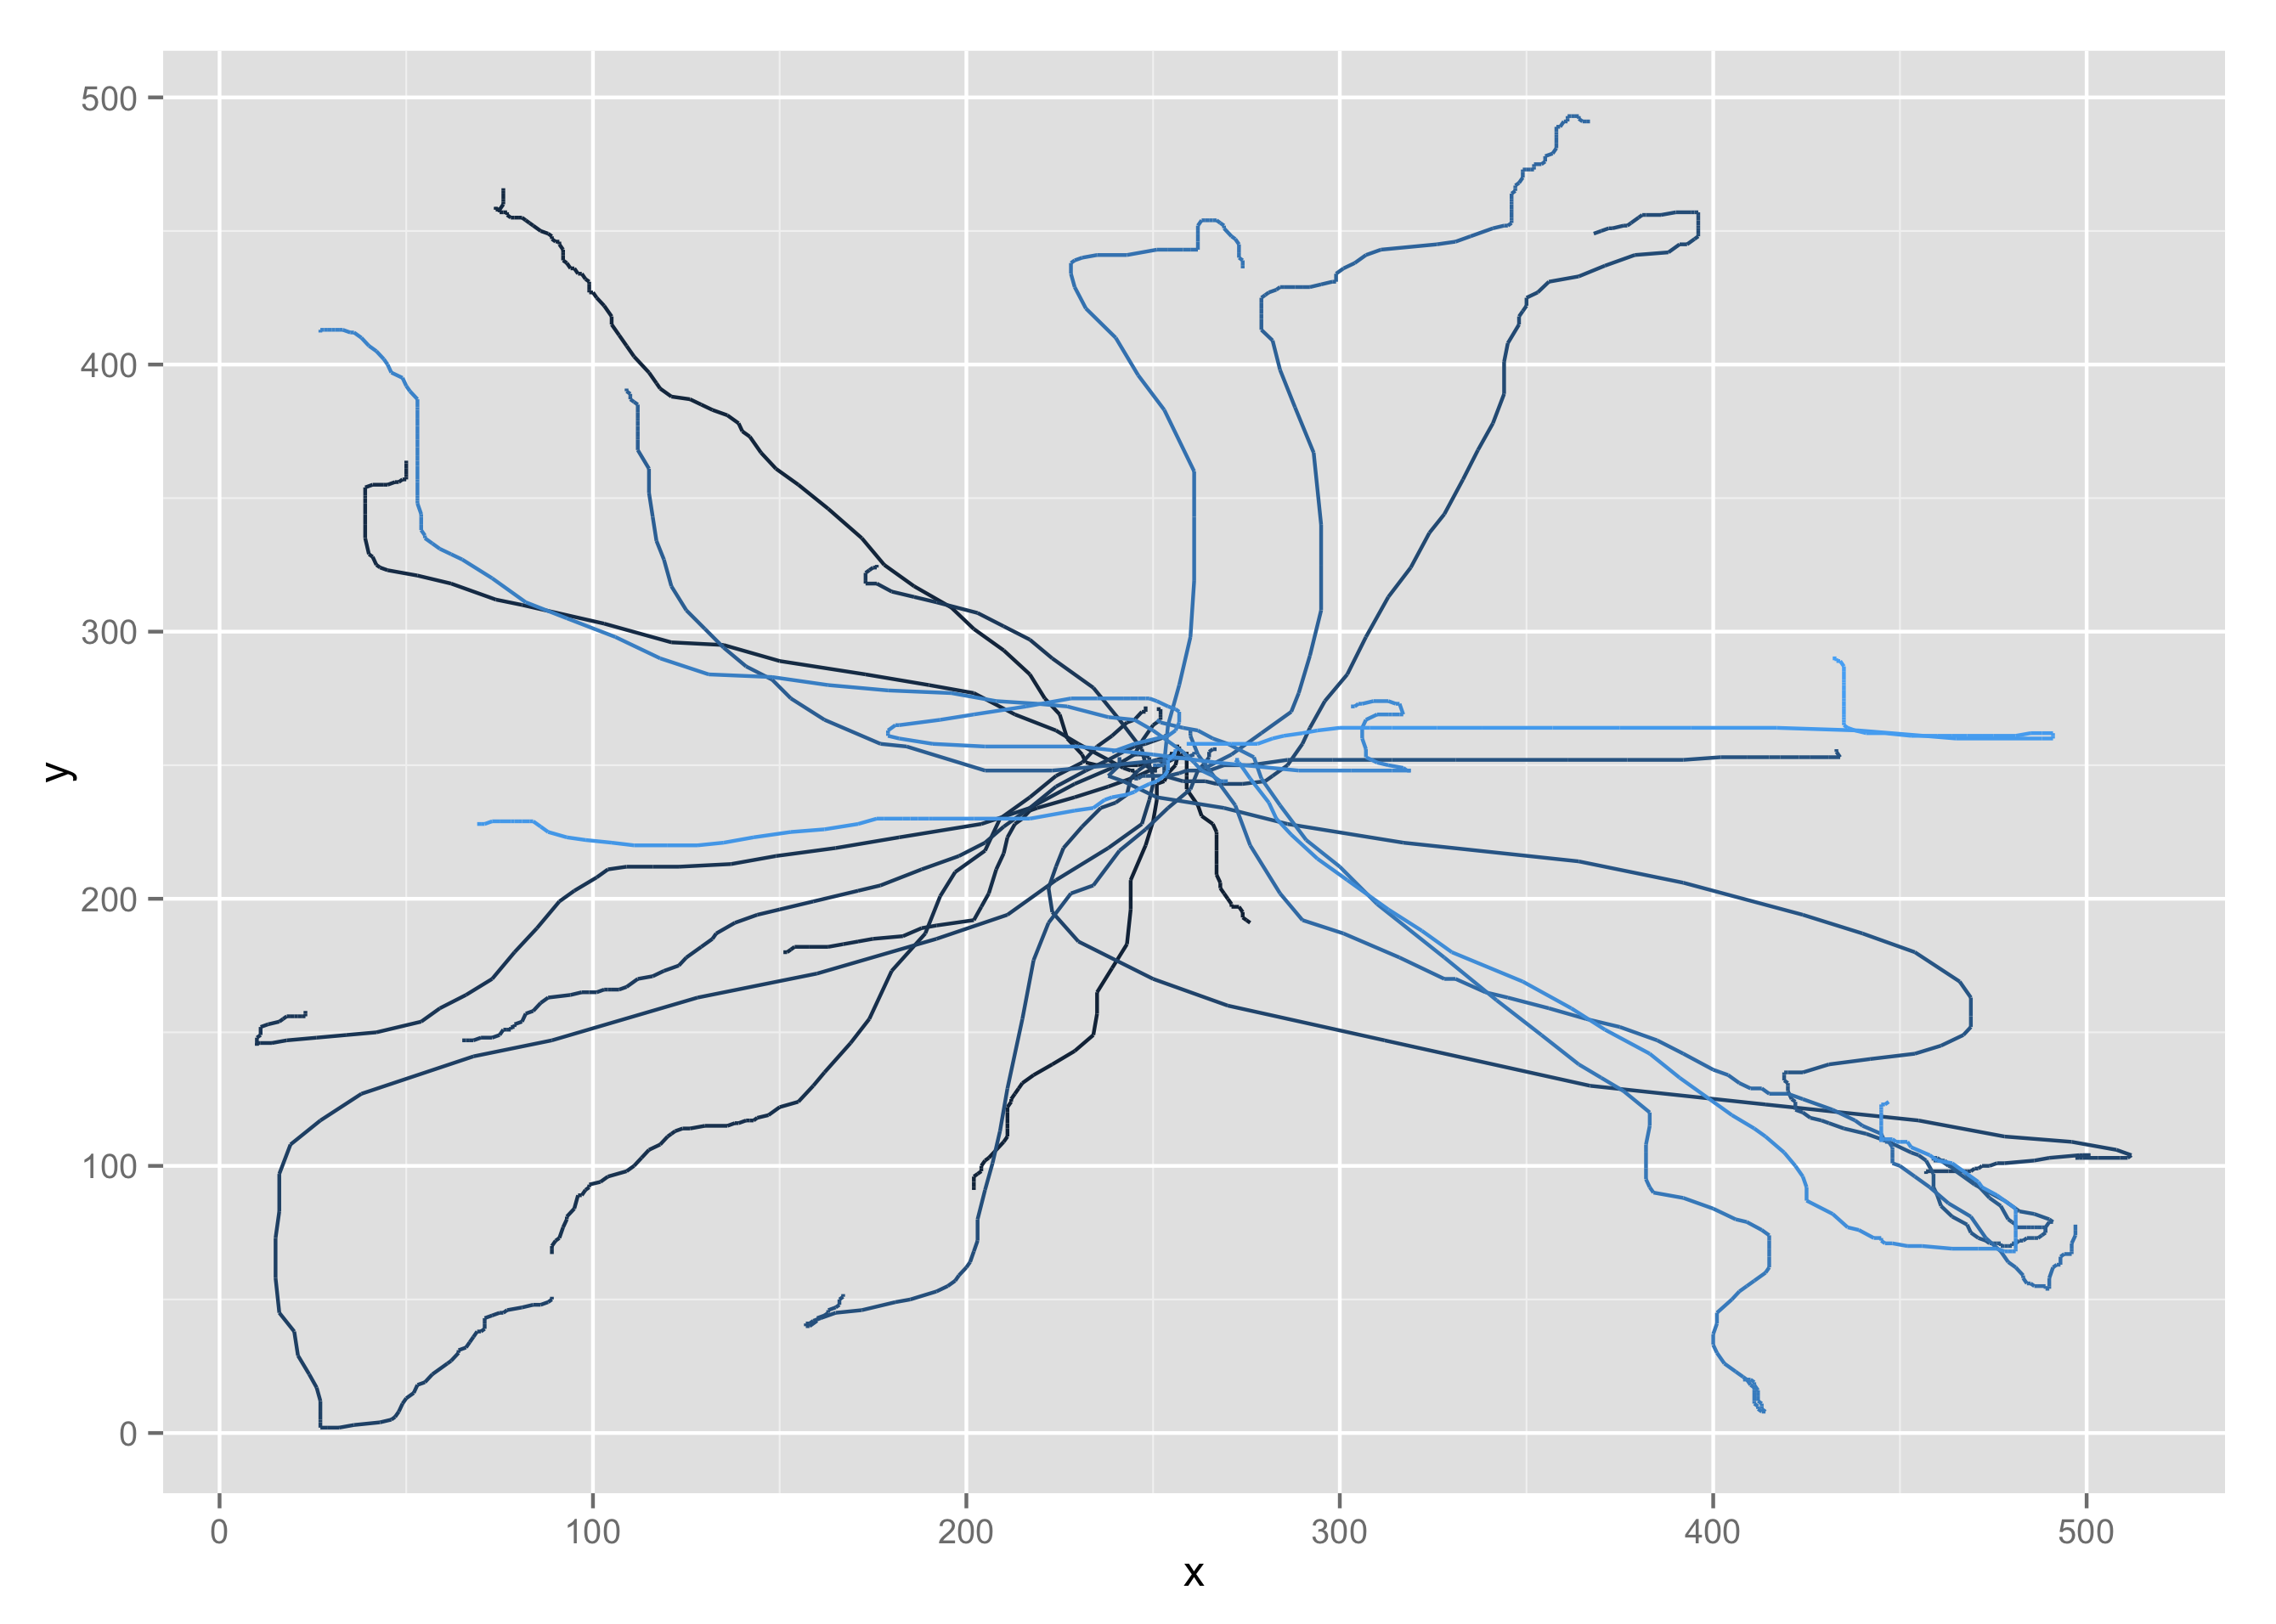
\includegraphics[width=\linewidth]{images/plots/plot_analysis_qualitative_77}
	\end{minipage}
	\begin{minipage}{0.5\linewidth}
		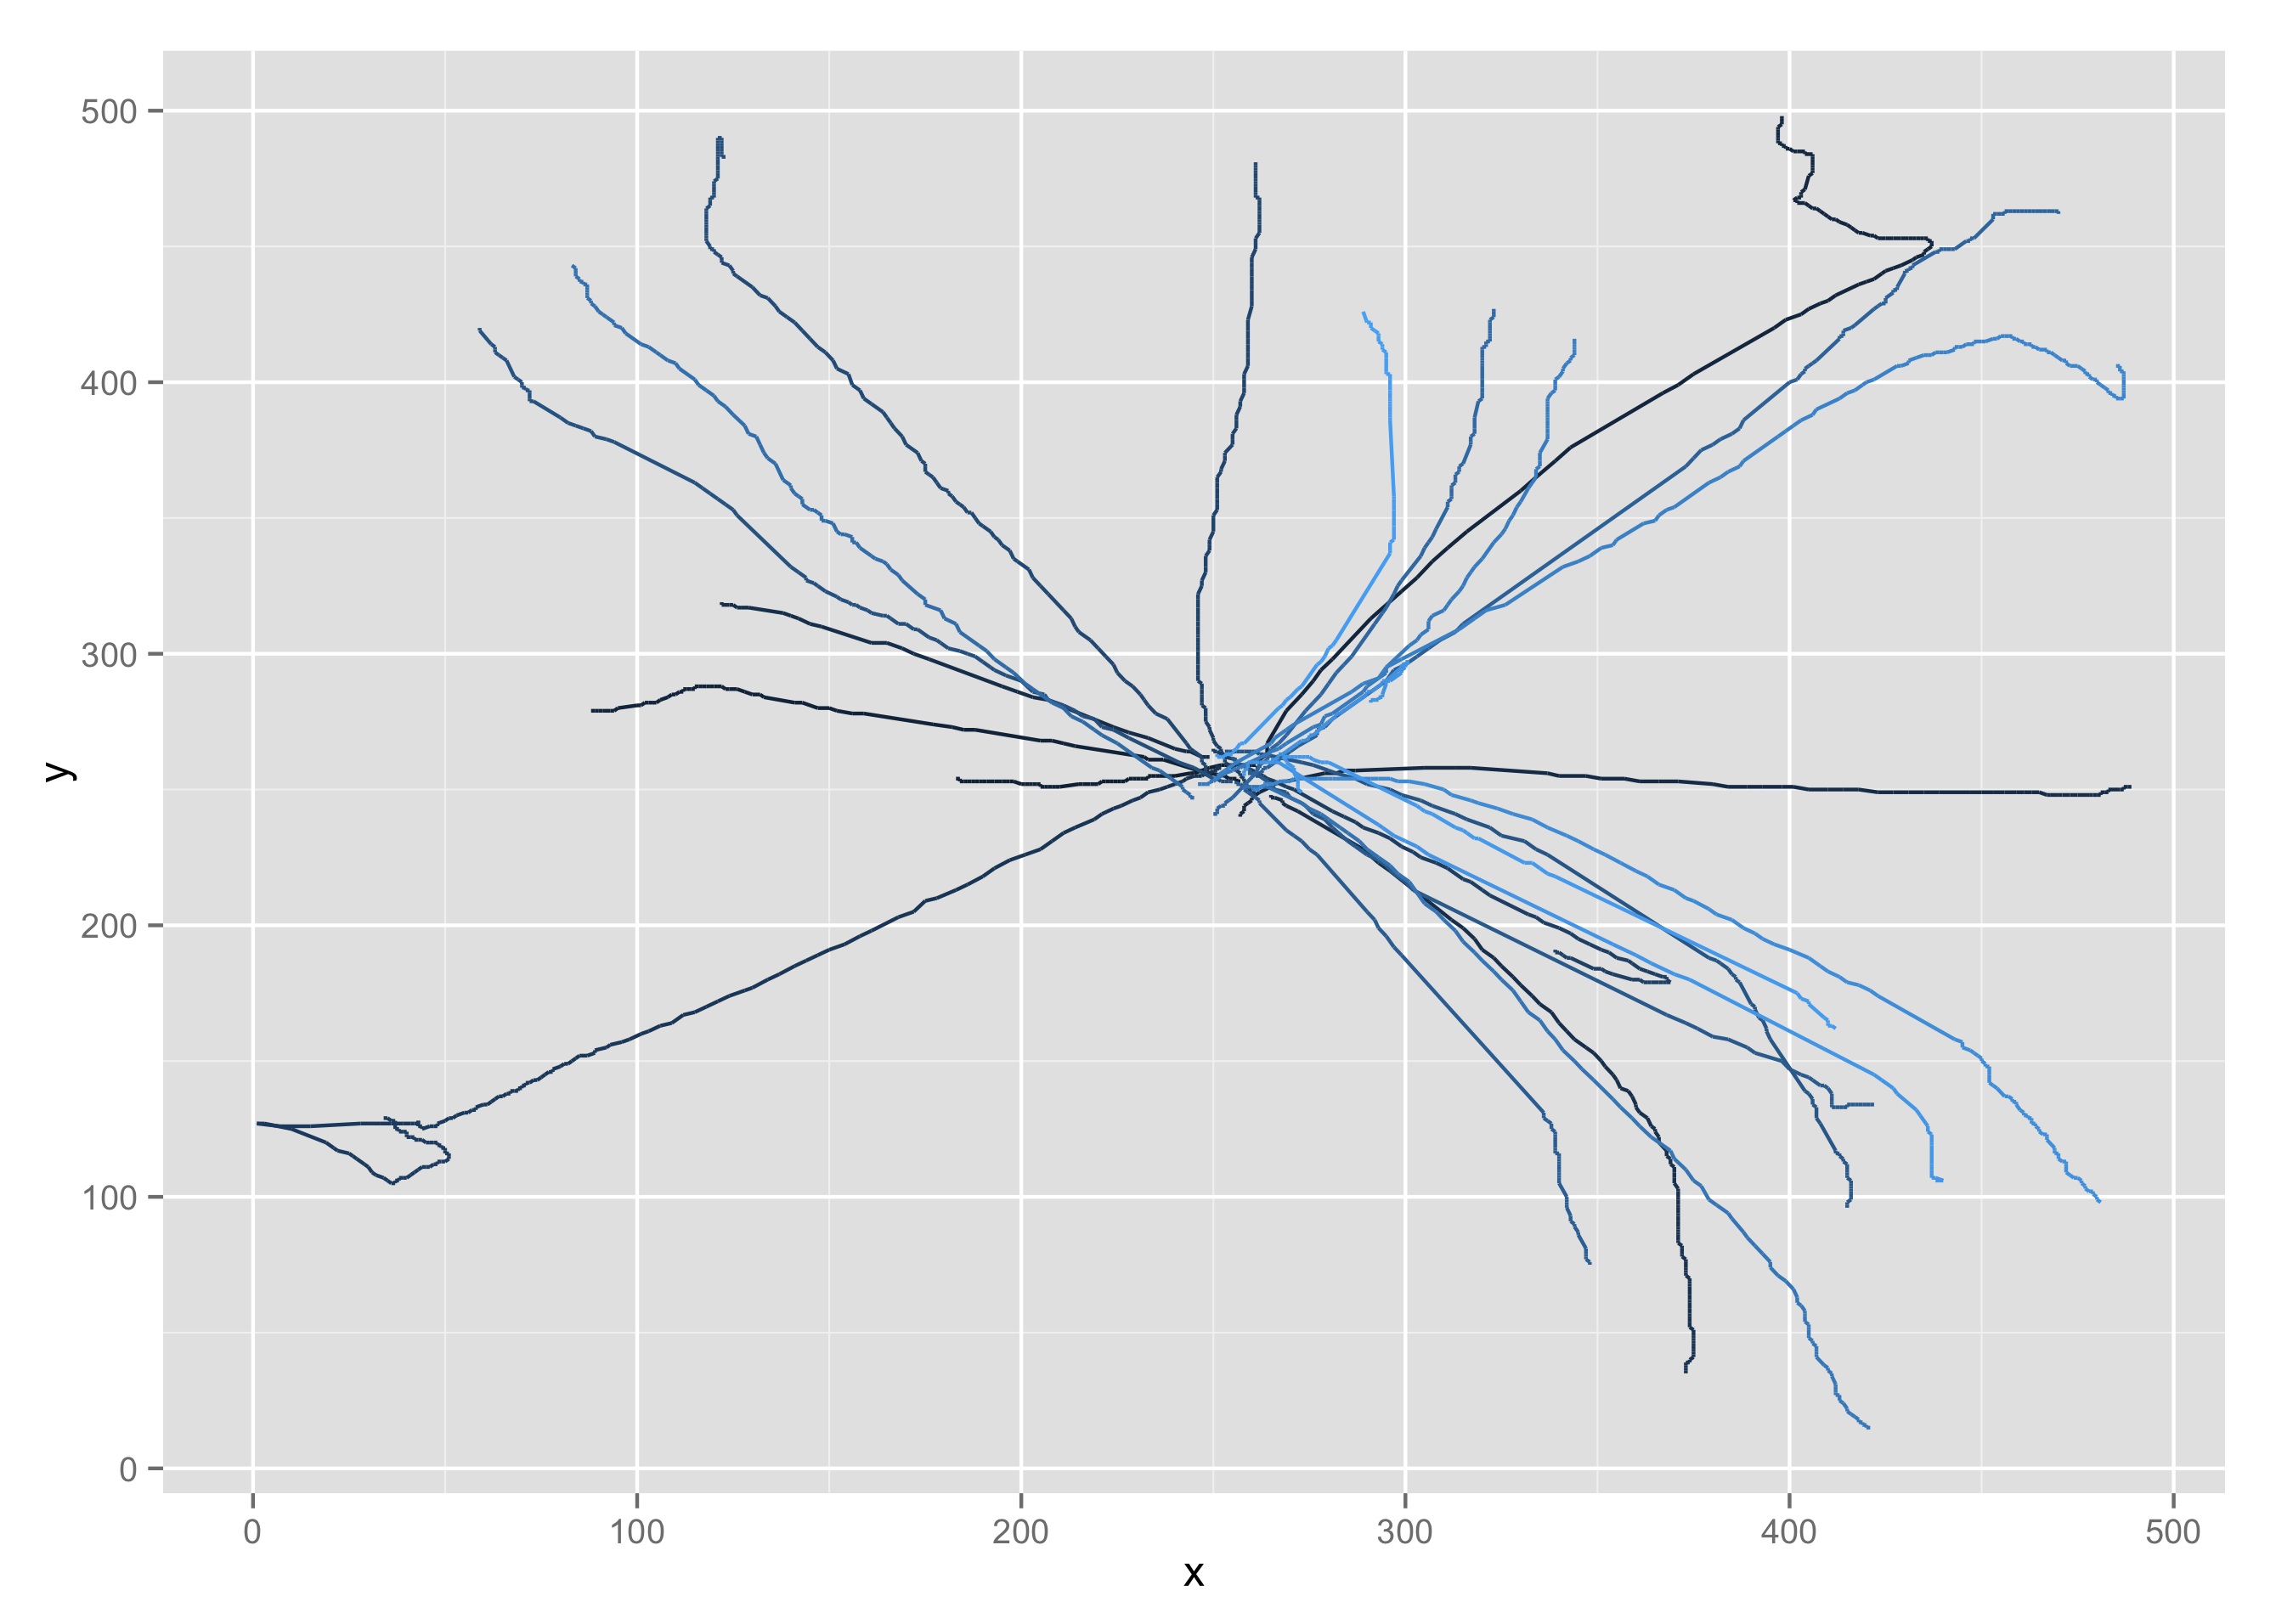
\includegraphics[width=\linewidth]{images/plots/plot_analysis_qualitative_45}
	\end{minipage}
	\begin{minipage}{0.5\linewidth}
		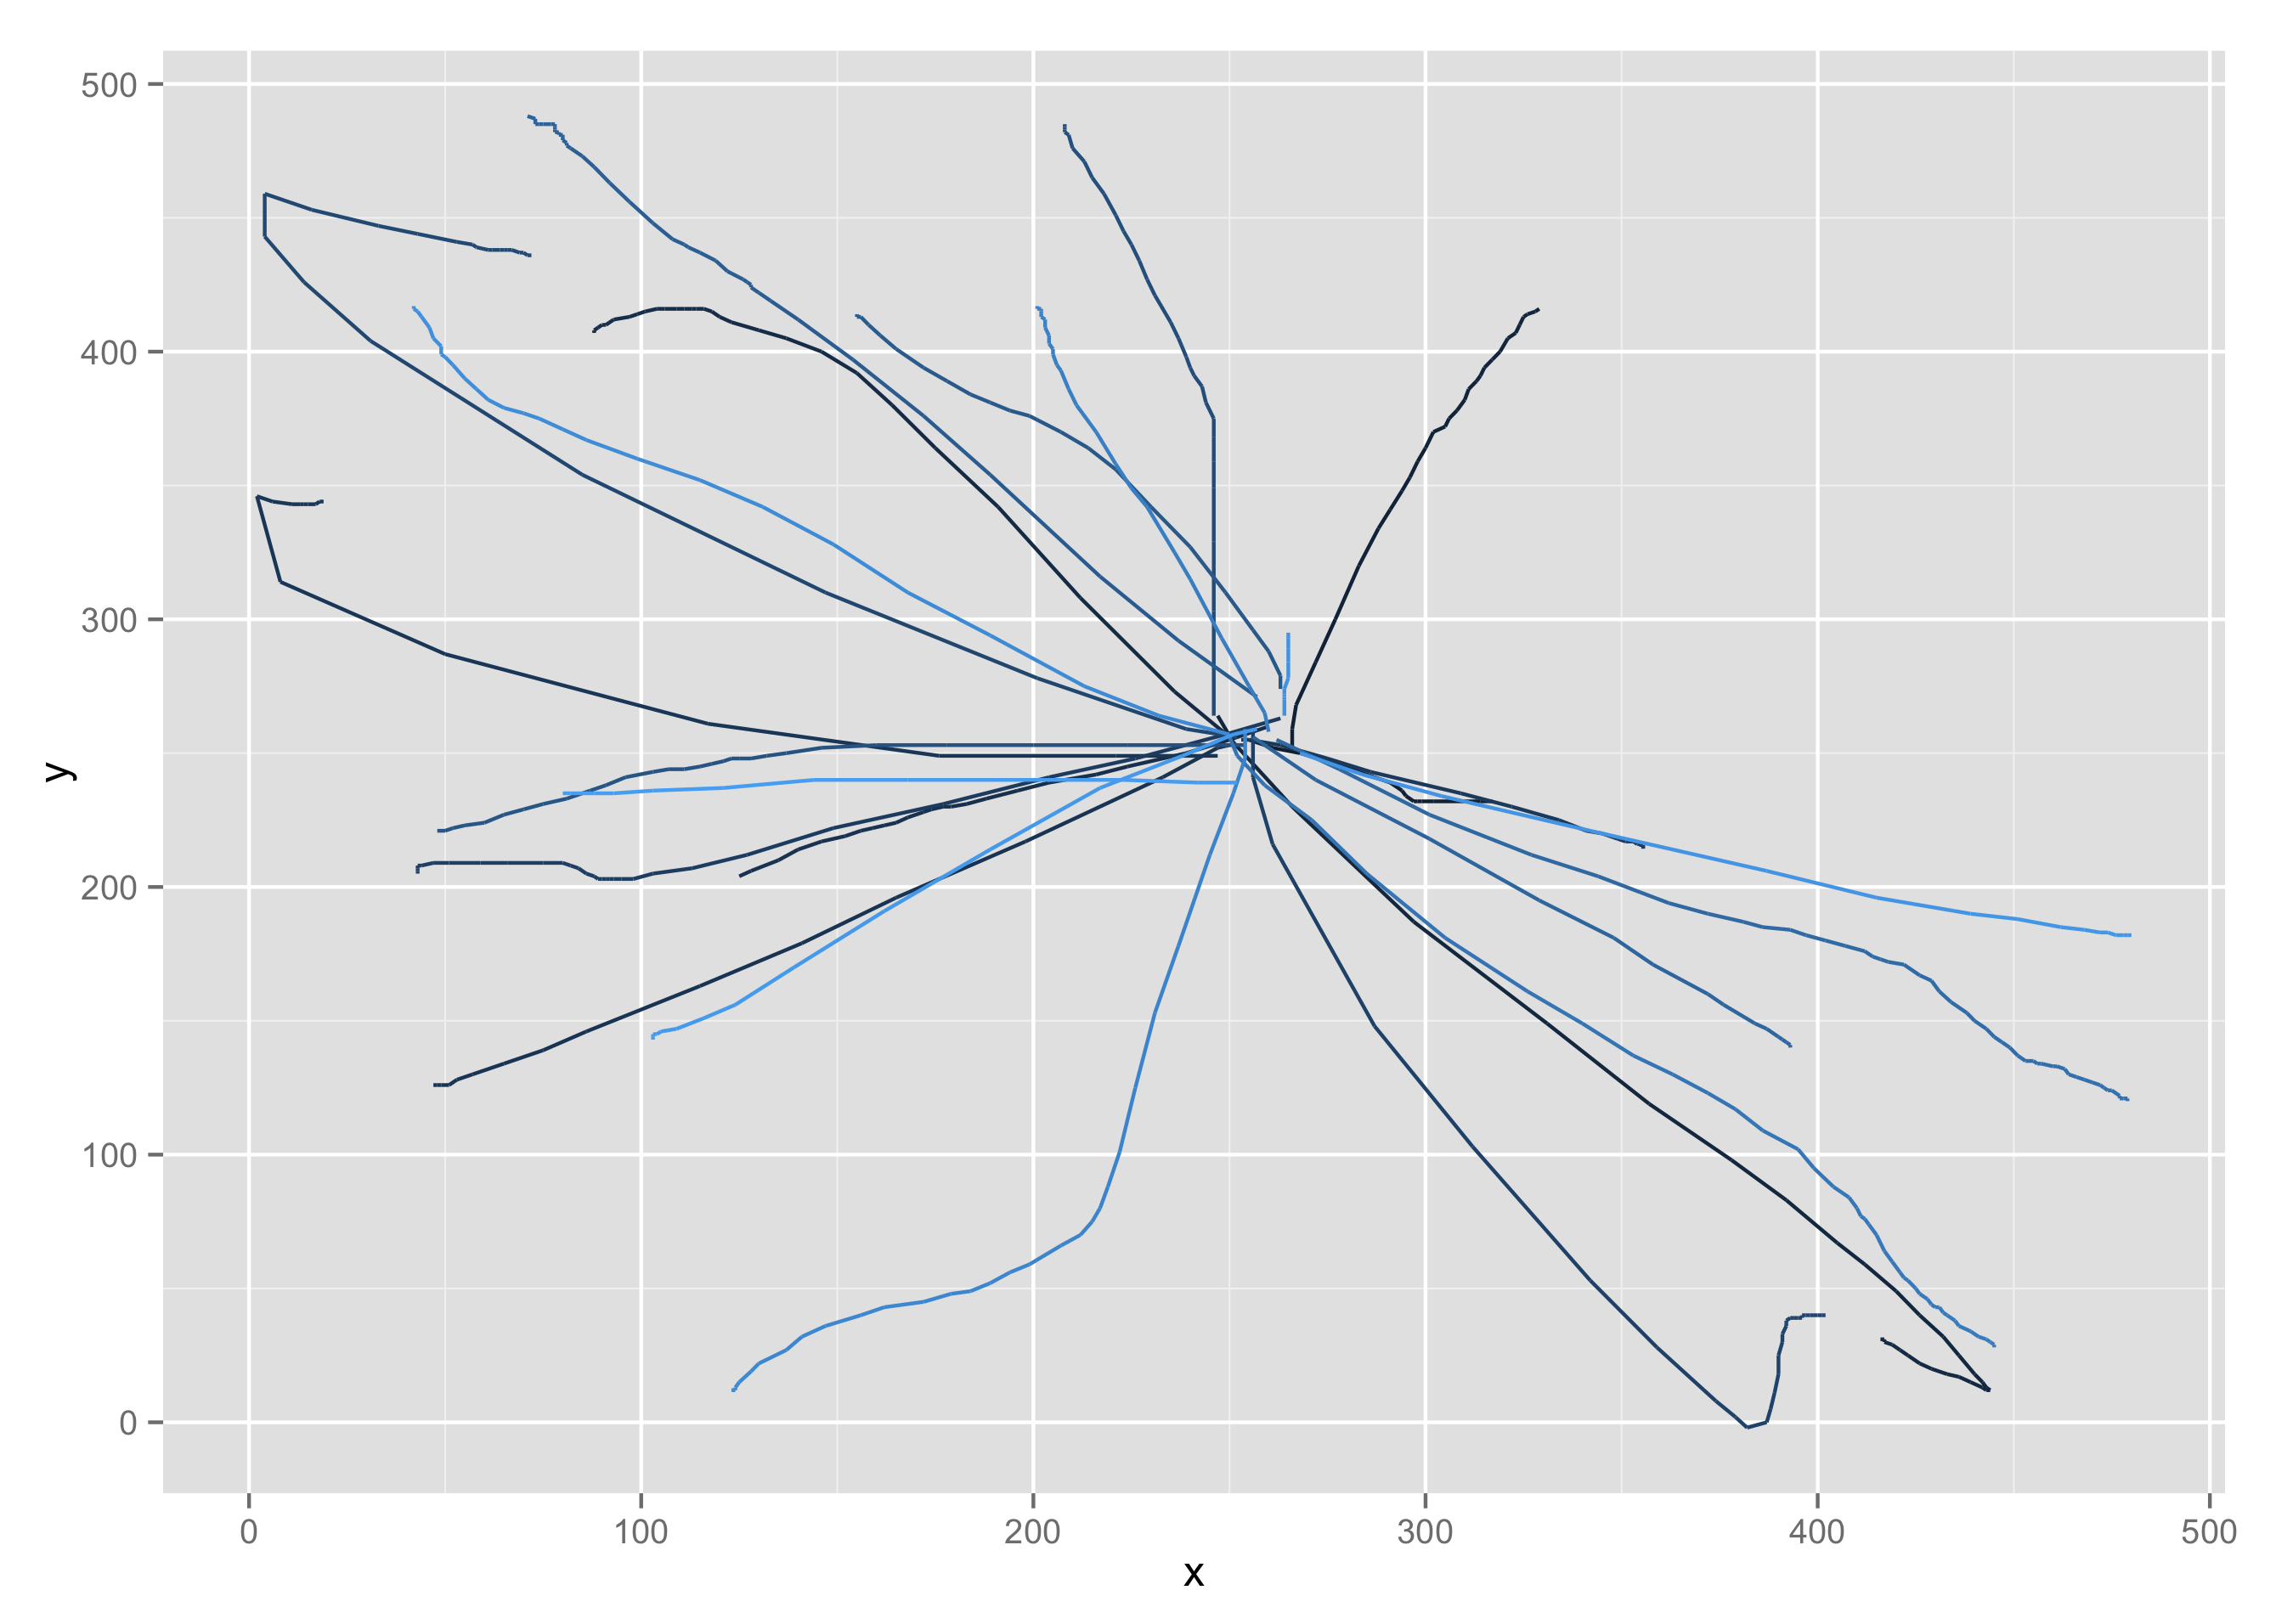
\includegraphics[width=\linewidth]{images/plots/plot_analysis_qualitative_225}
	\end{minipage}
	\begin{minipage}{0.5\linewidth}
		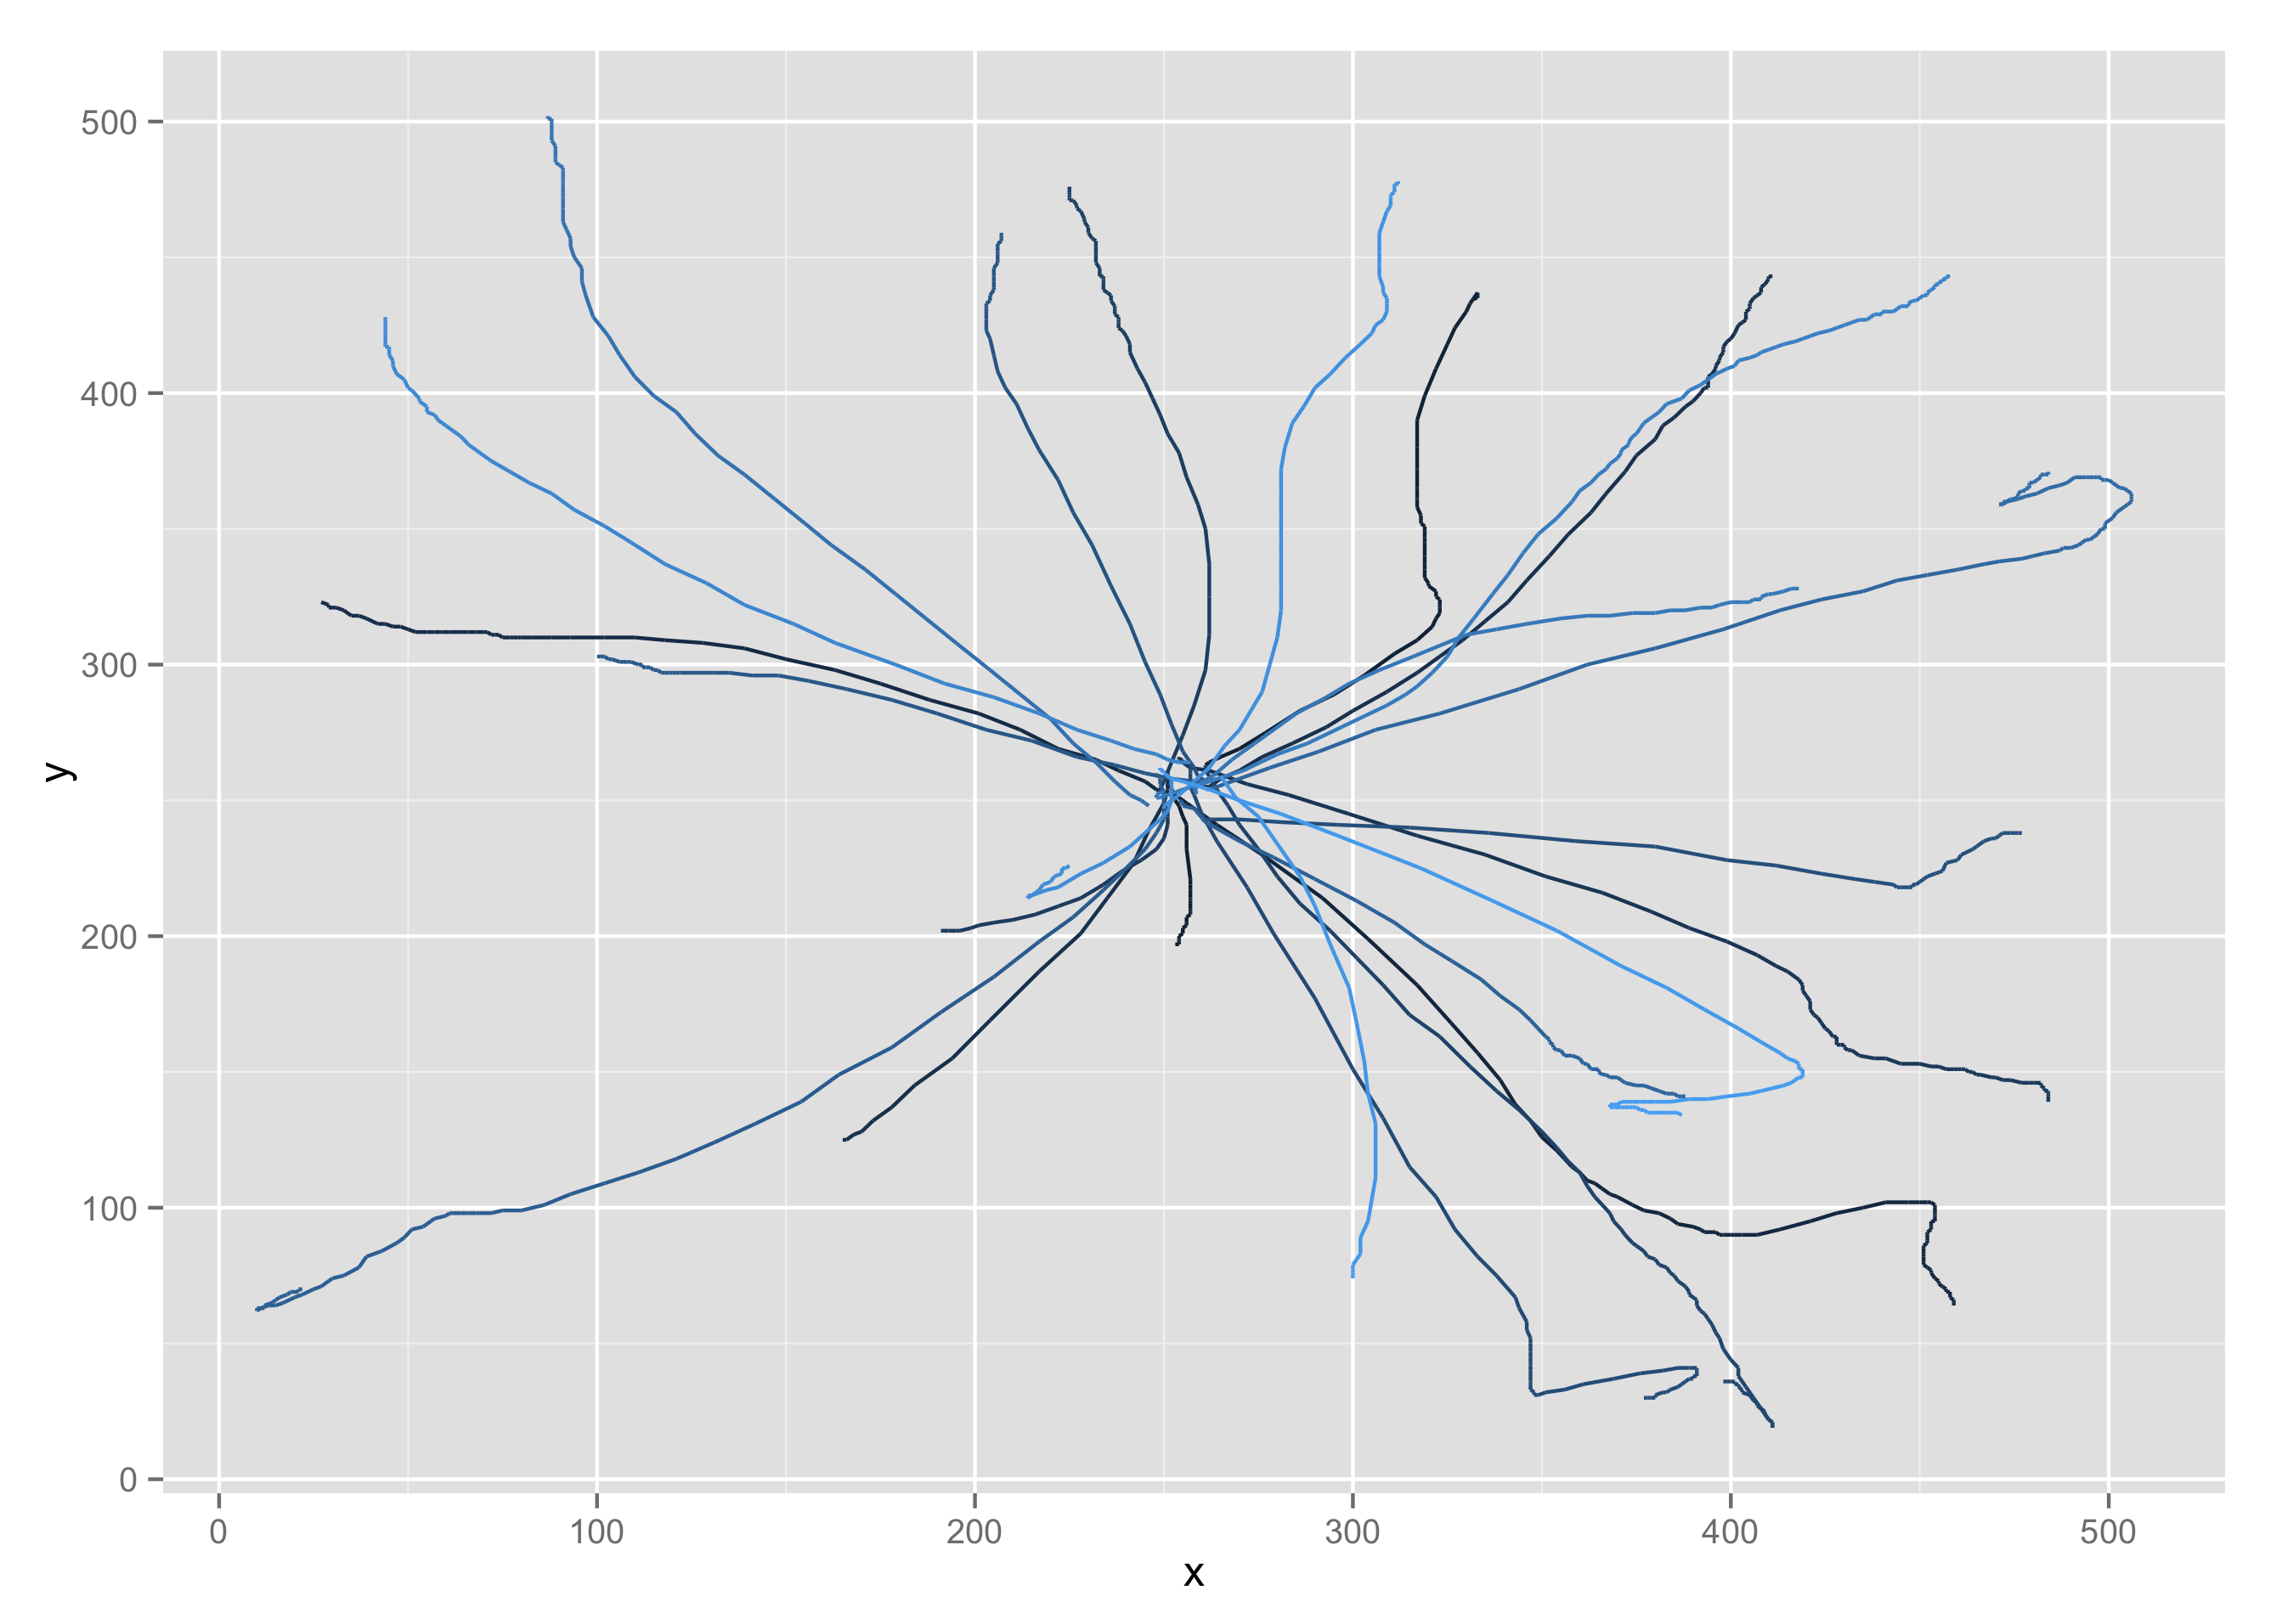
\includegraphics[width=\linewidth]{images/plots/plot_analysis_qualitative_161}
	\end{minipage}
	\begin{minipage}{0.5\linewidth}
		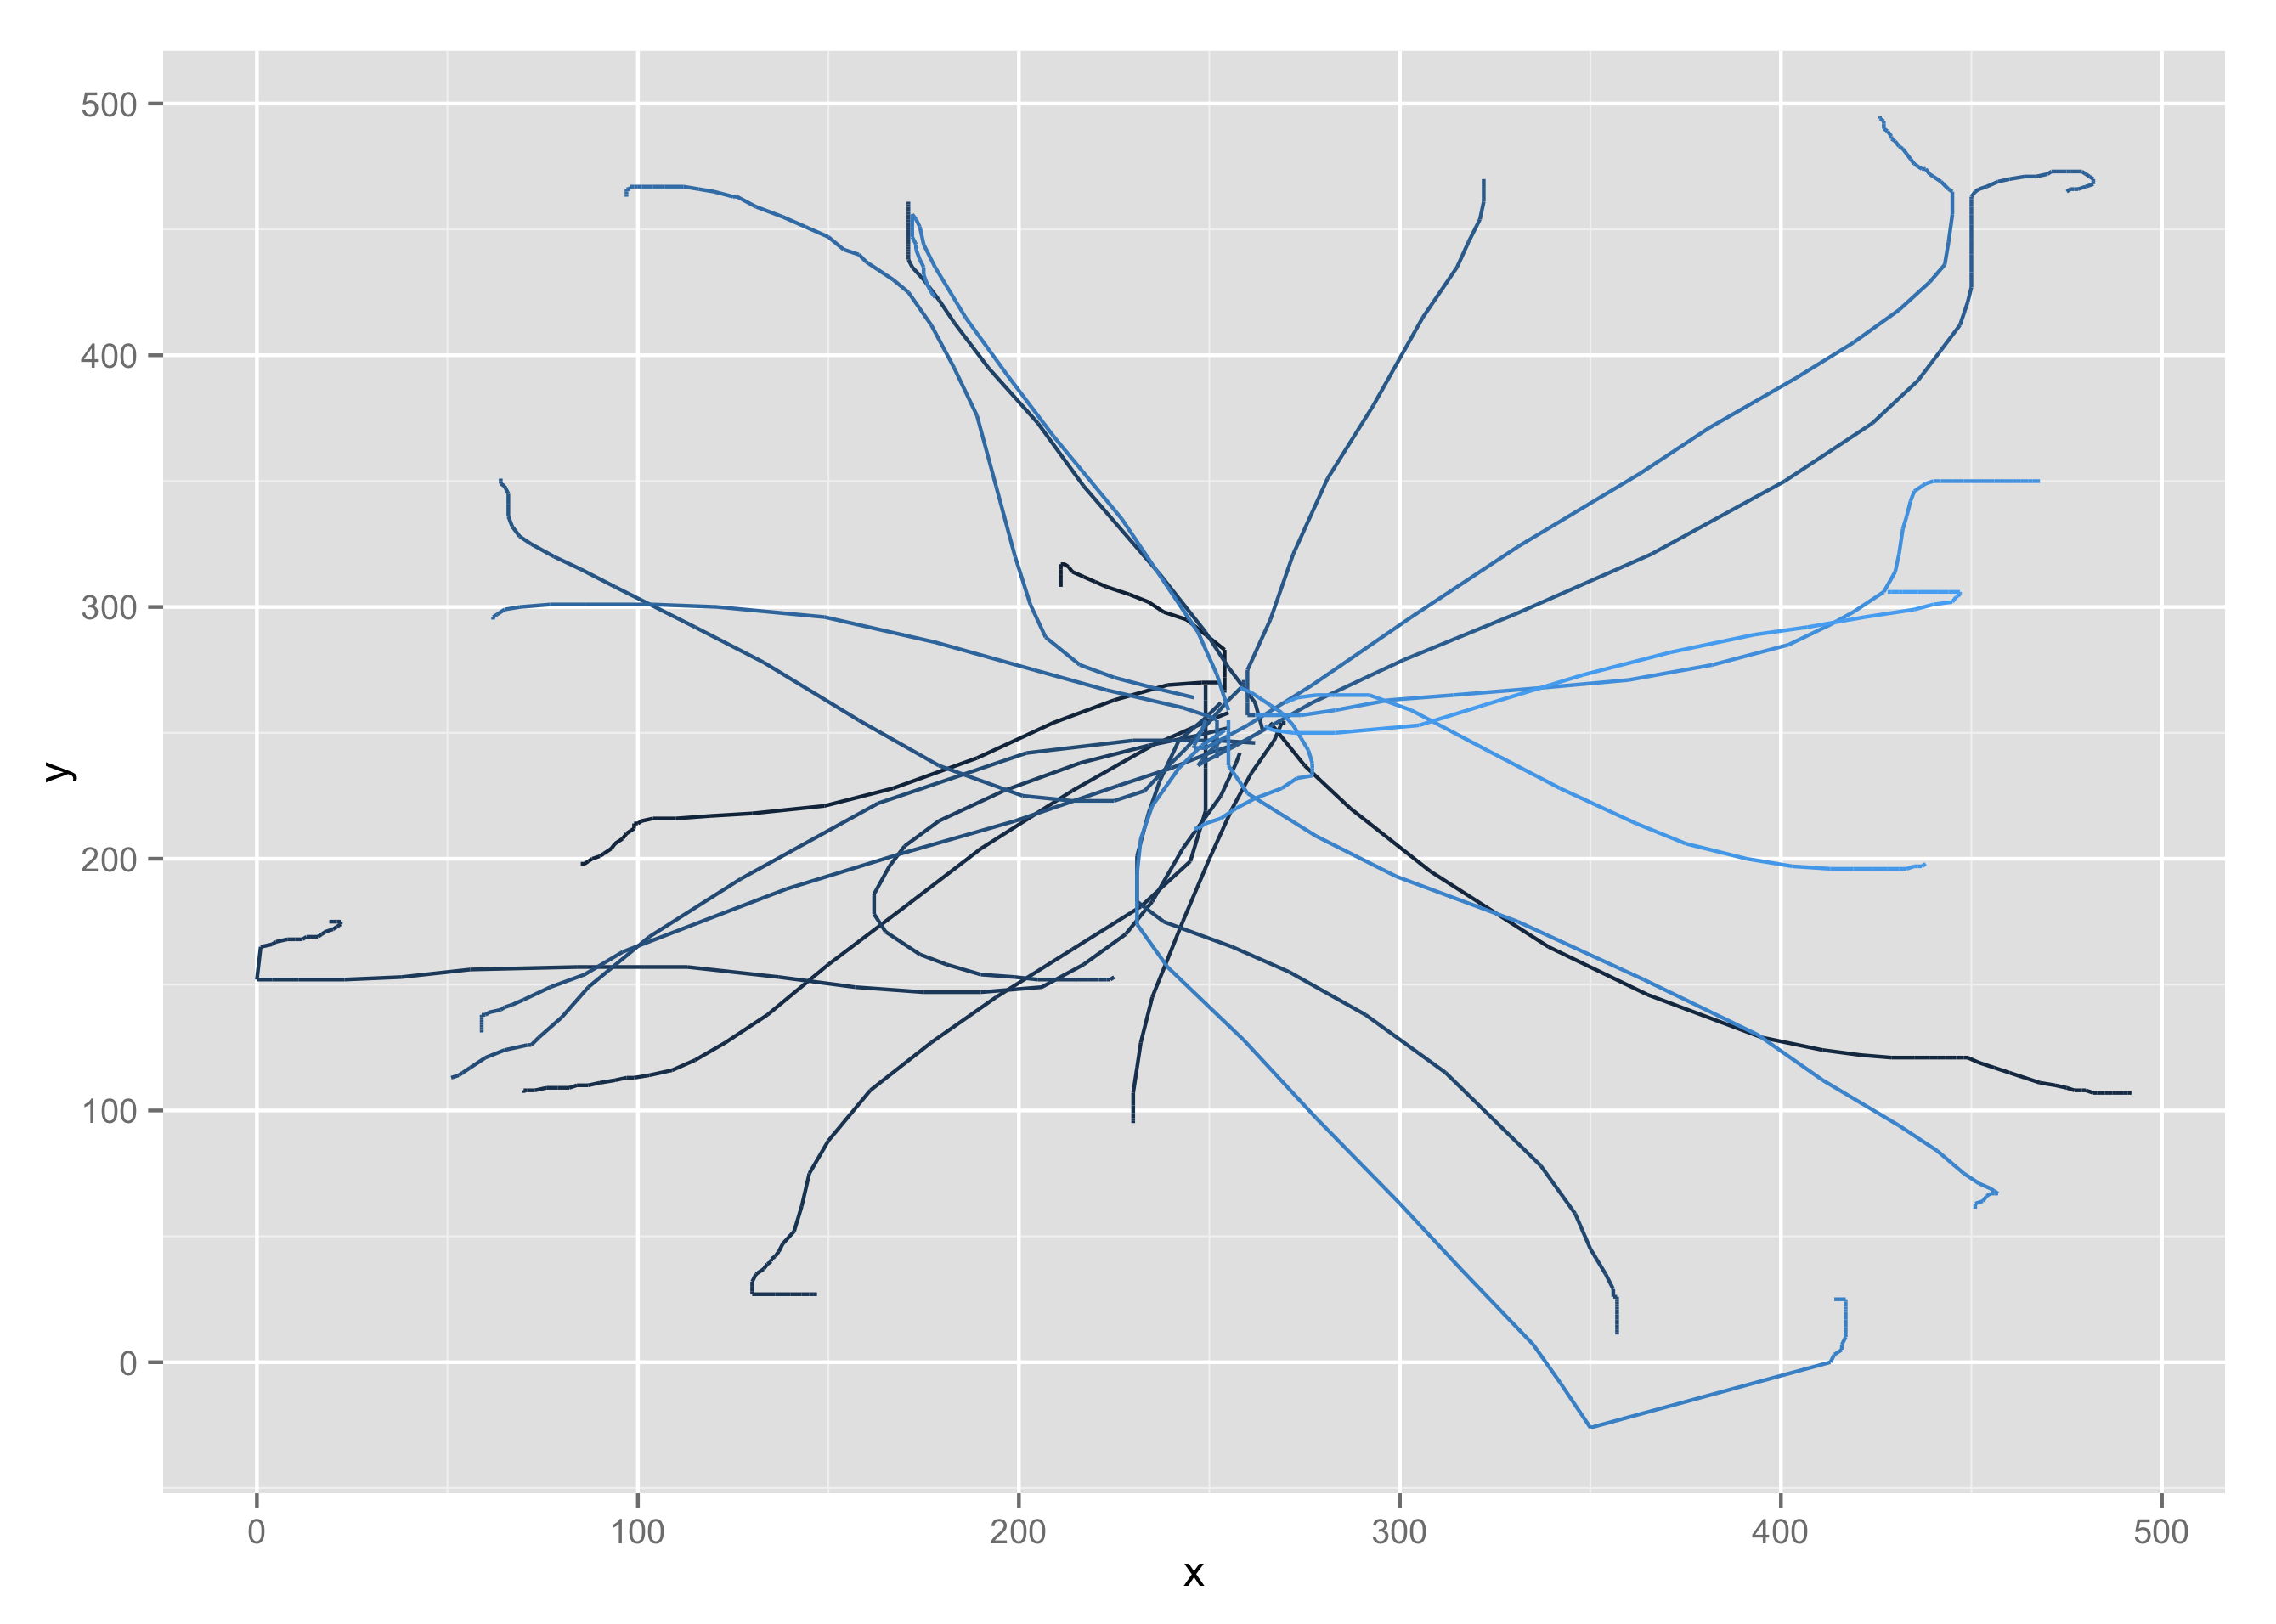
\includegraphics[width=\linewidth]{images/plots/plot_analysis_qualitative_235}
	\end{minipage}
	\begin{minipage}{0.5\linewidth}
		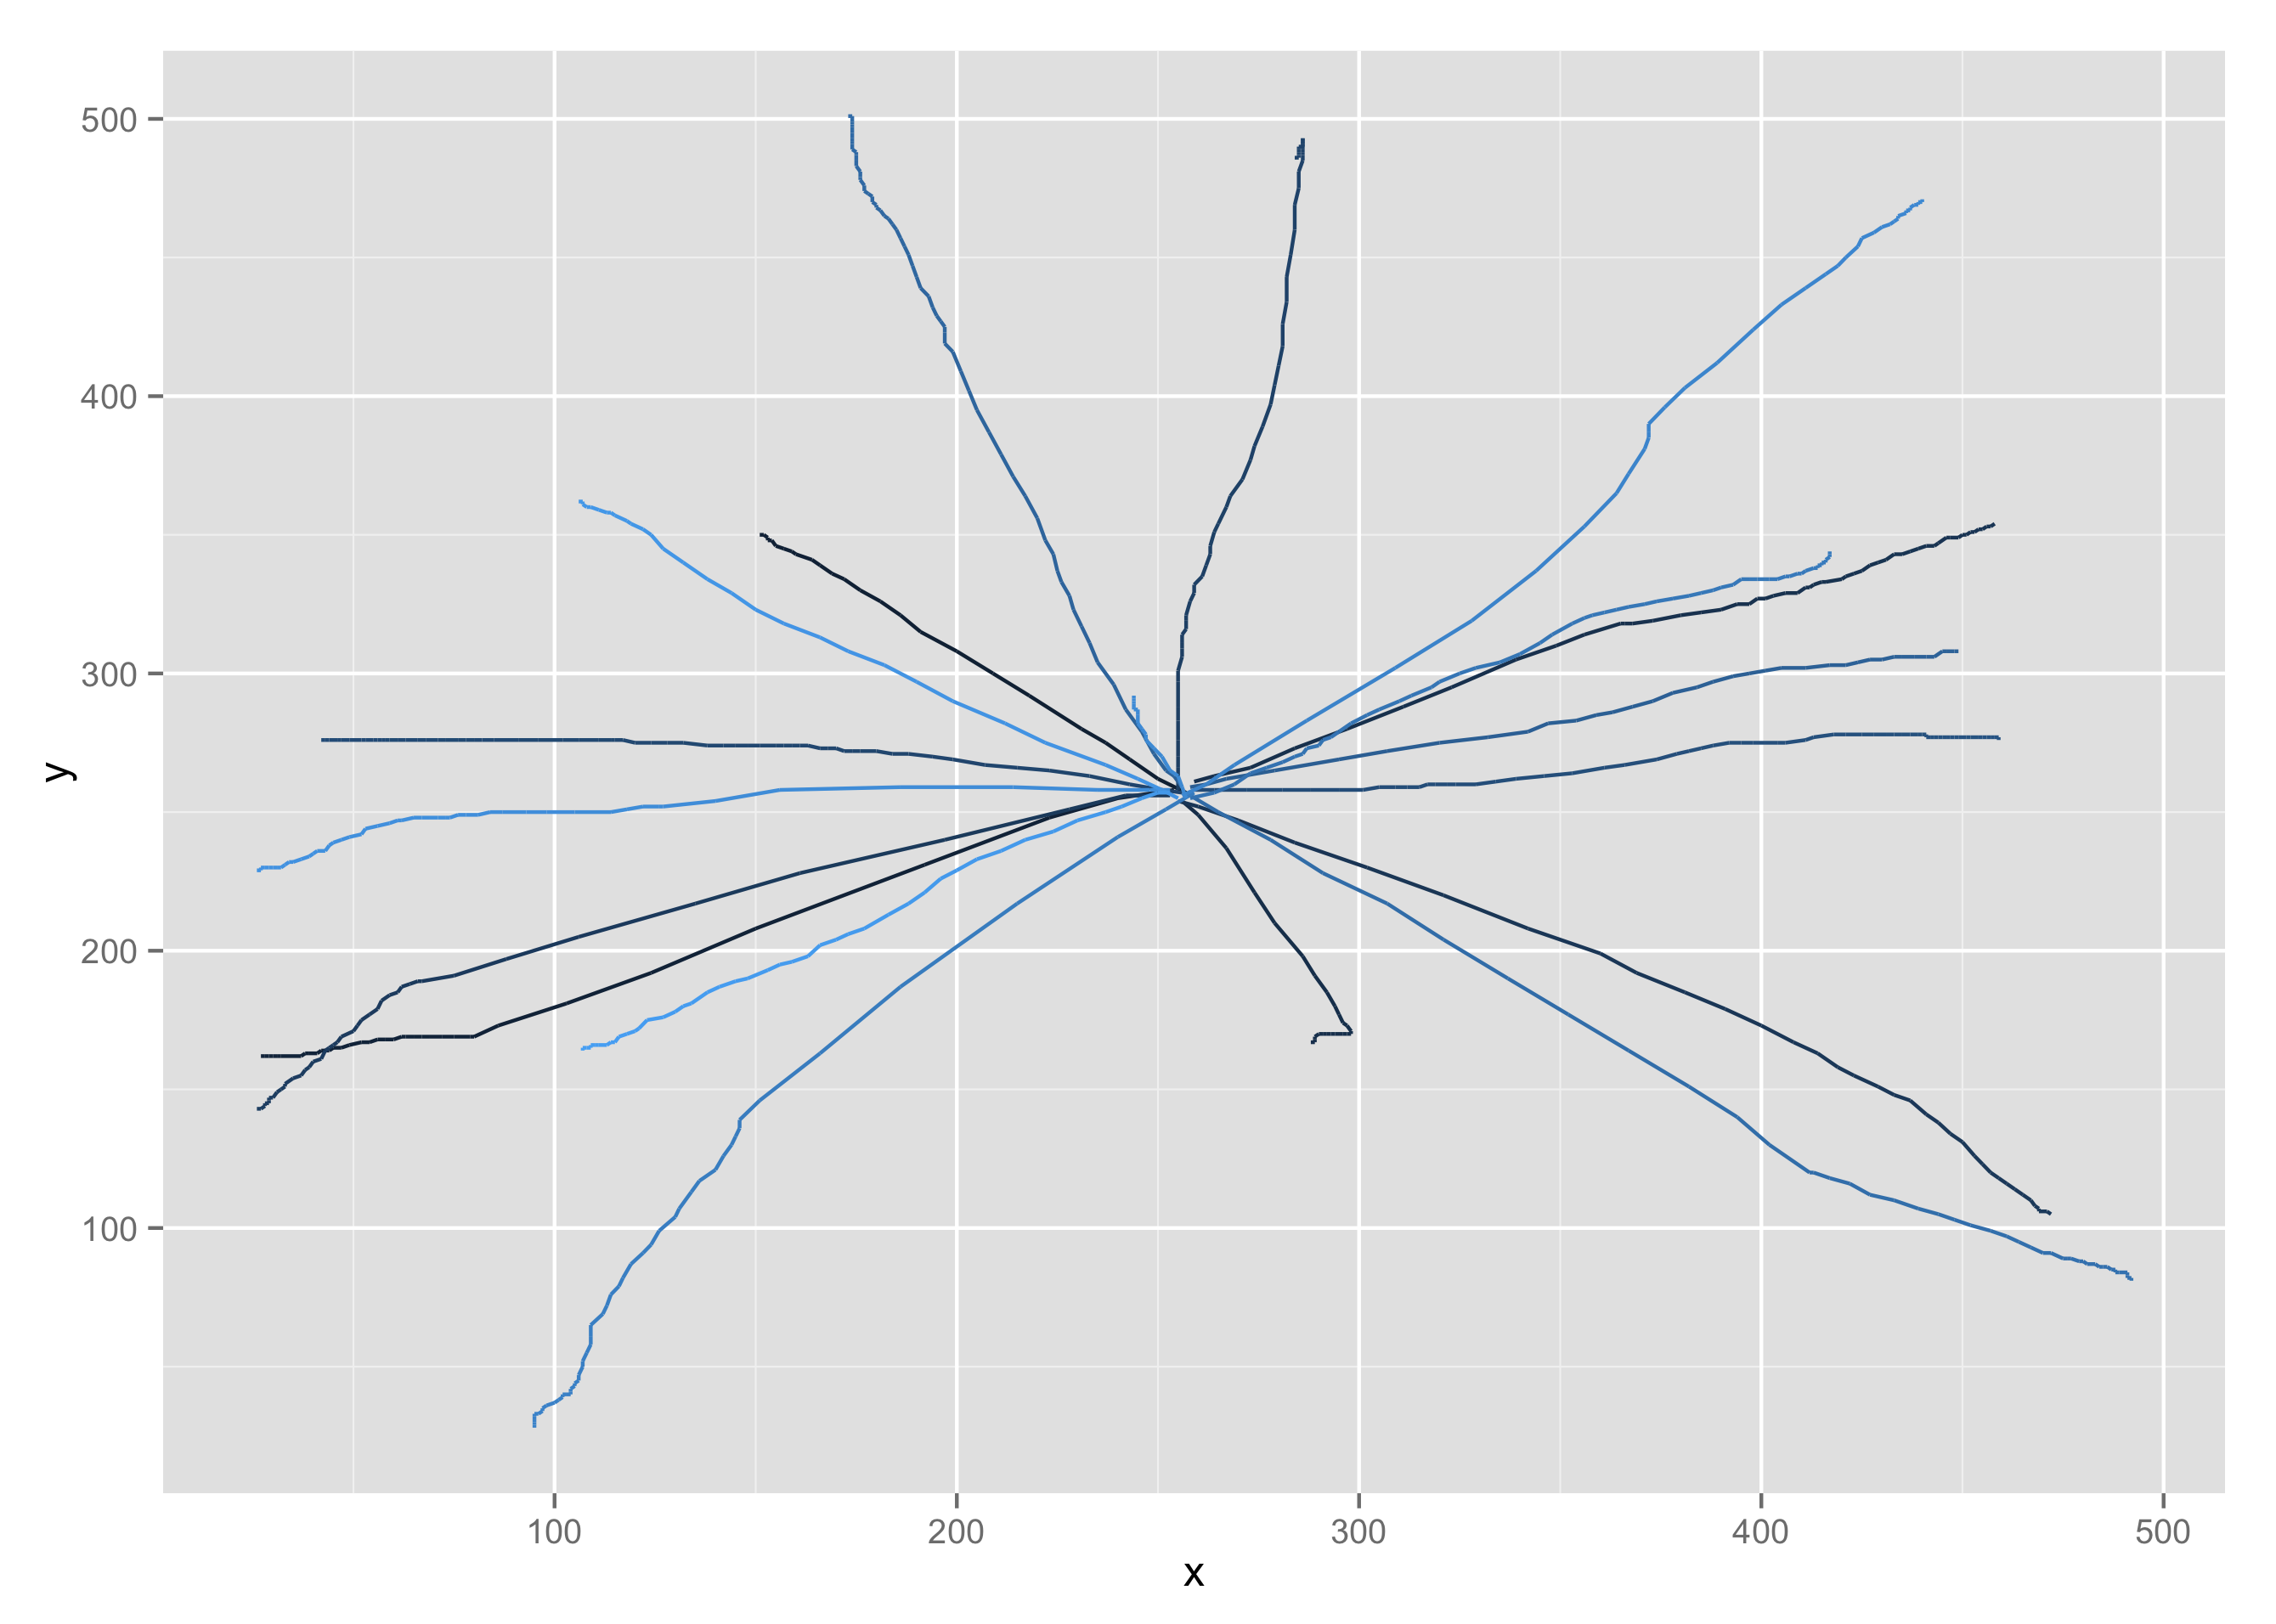
\includegraphics[width=\linewidth]{images/plots/plot_analysis_qualitative_239}
	\end{minipage}	
	\captionof{figure}{6 testdeltageres bevægelsesbaner for de 25 pegeopgaver}
	\label{fig:kvaliativ_persons_1}
\end{minipage}

\begin{minipage}{\textwidth}
	\begin{minipage}{0.5\linewidth}
		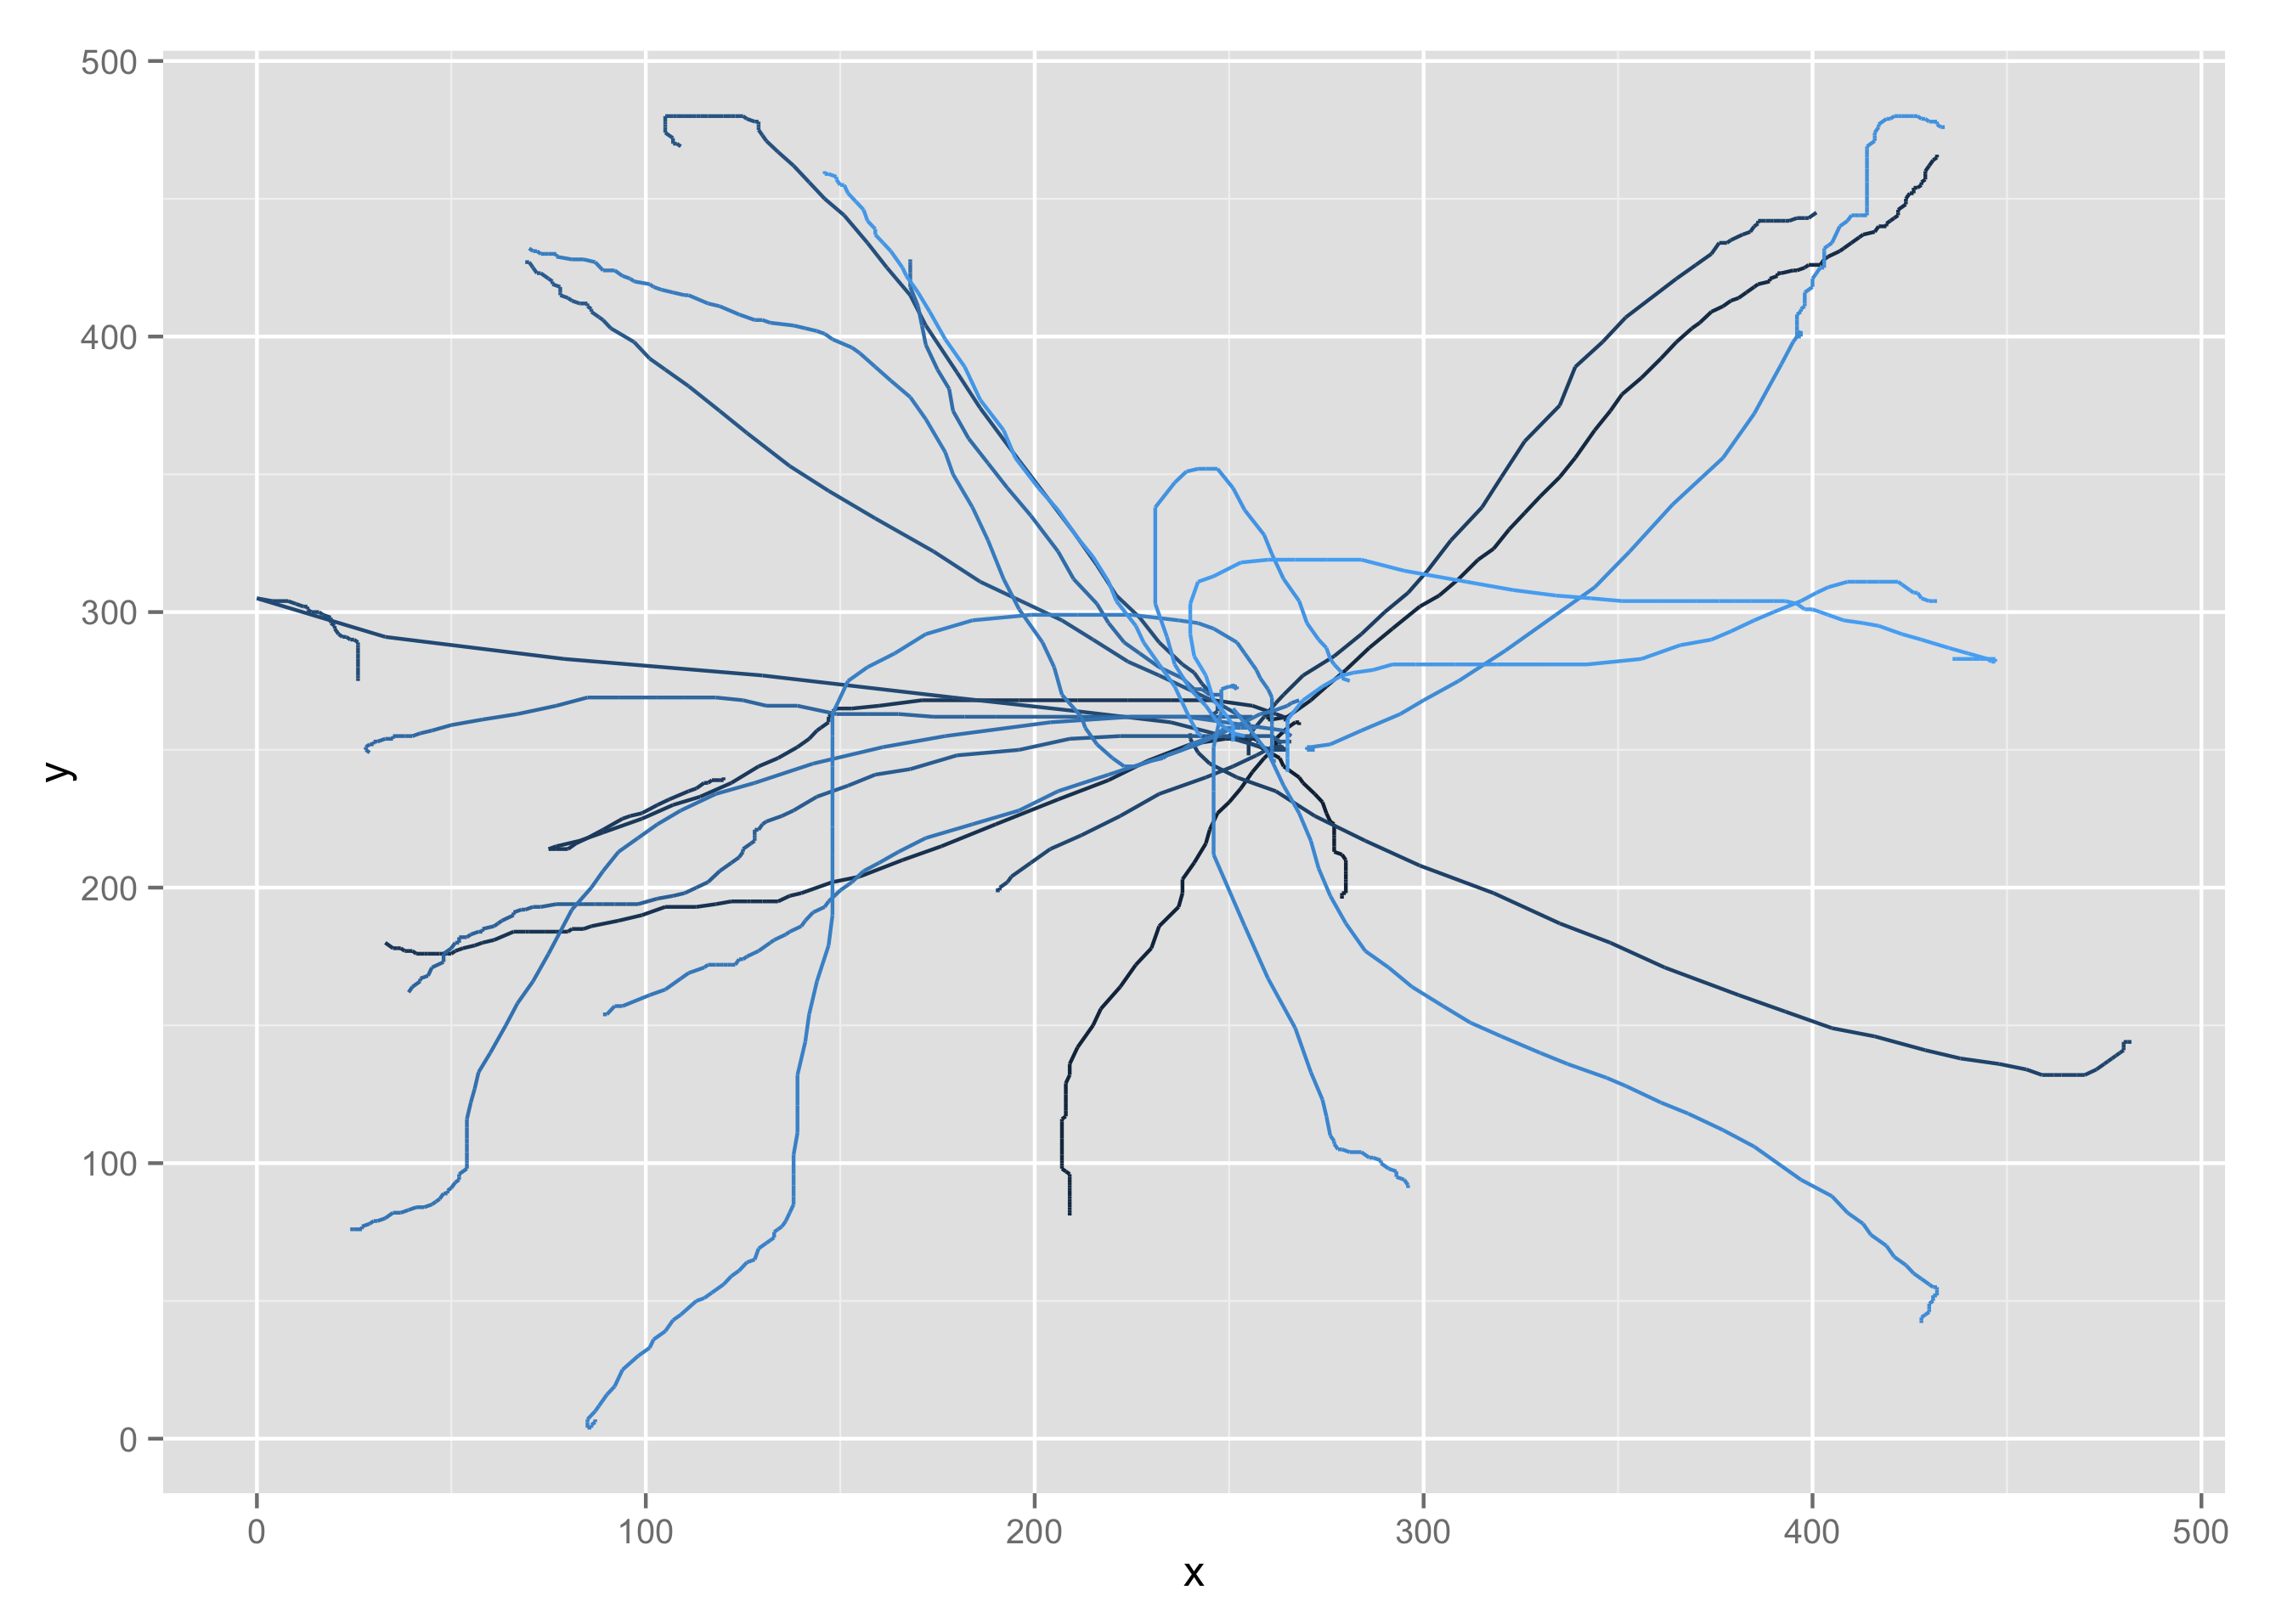
\includegraphics[width=\linewidth]{images/plots/plot_analysis_qualitative_113}
	\end{minipage}
	\begin{minipage}{0.5\linewidth}
		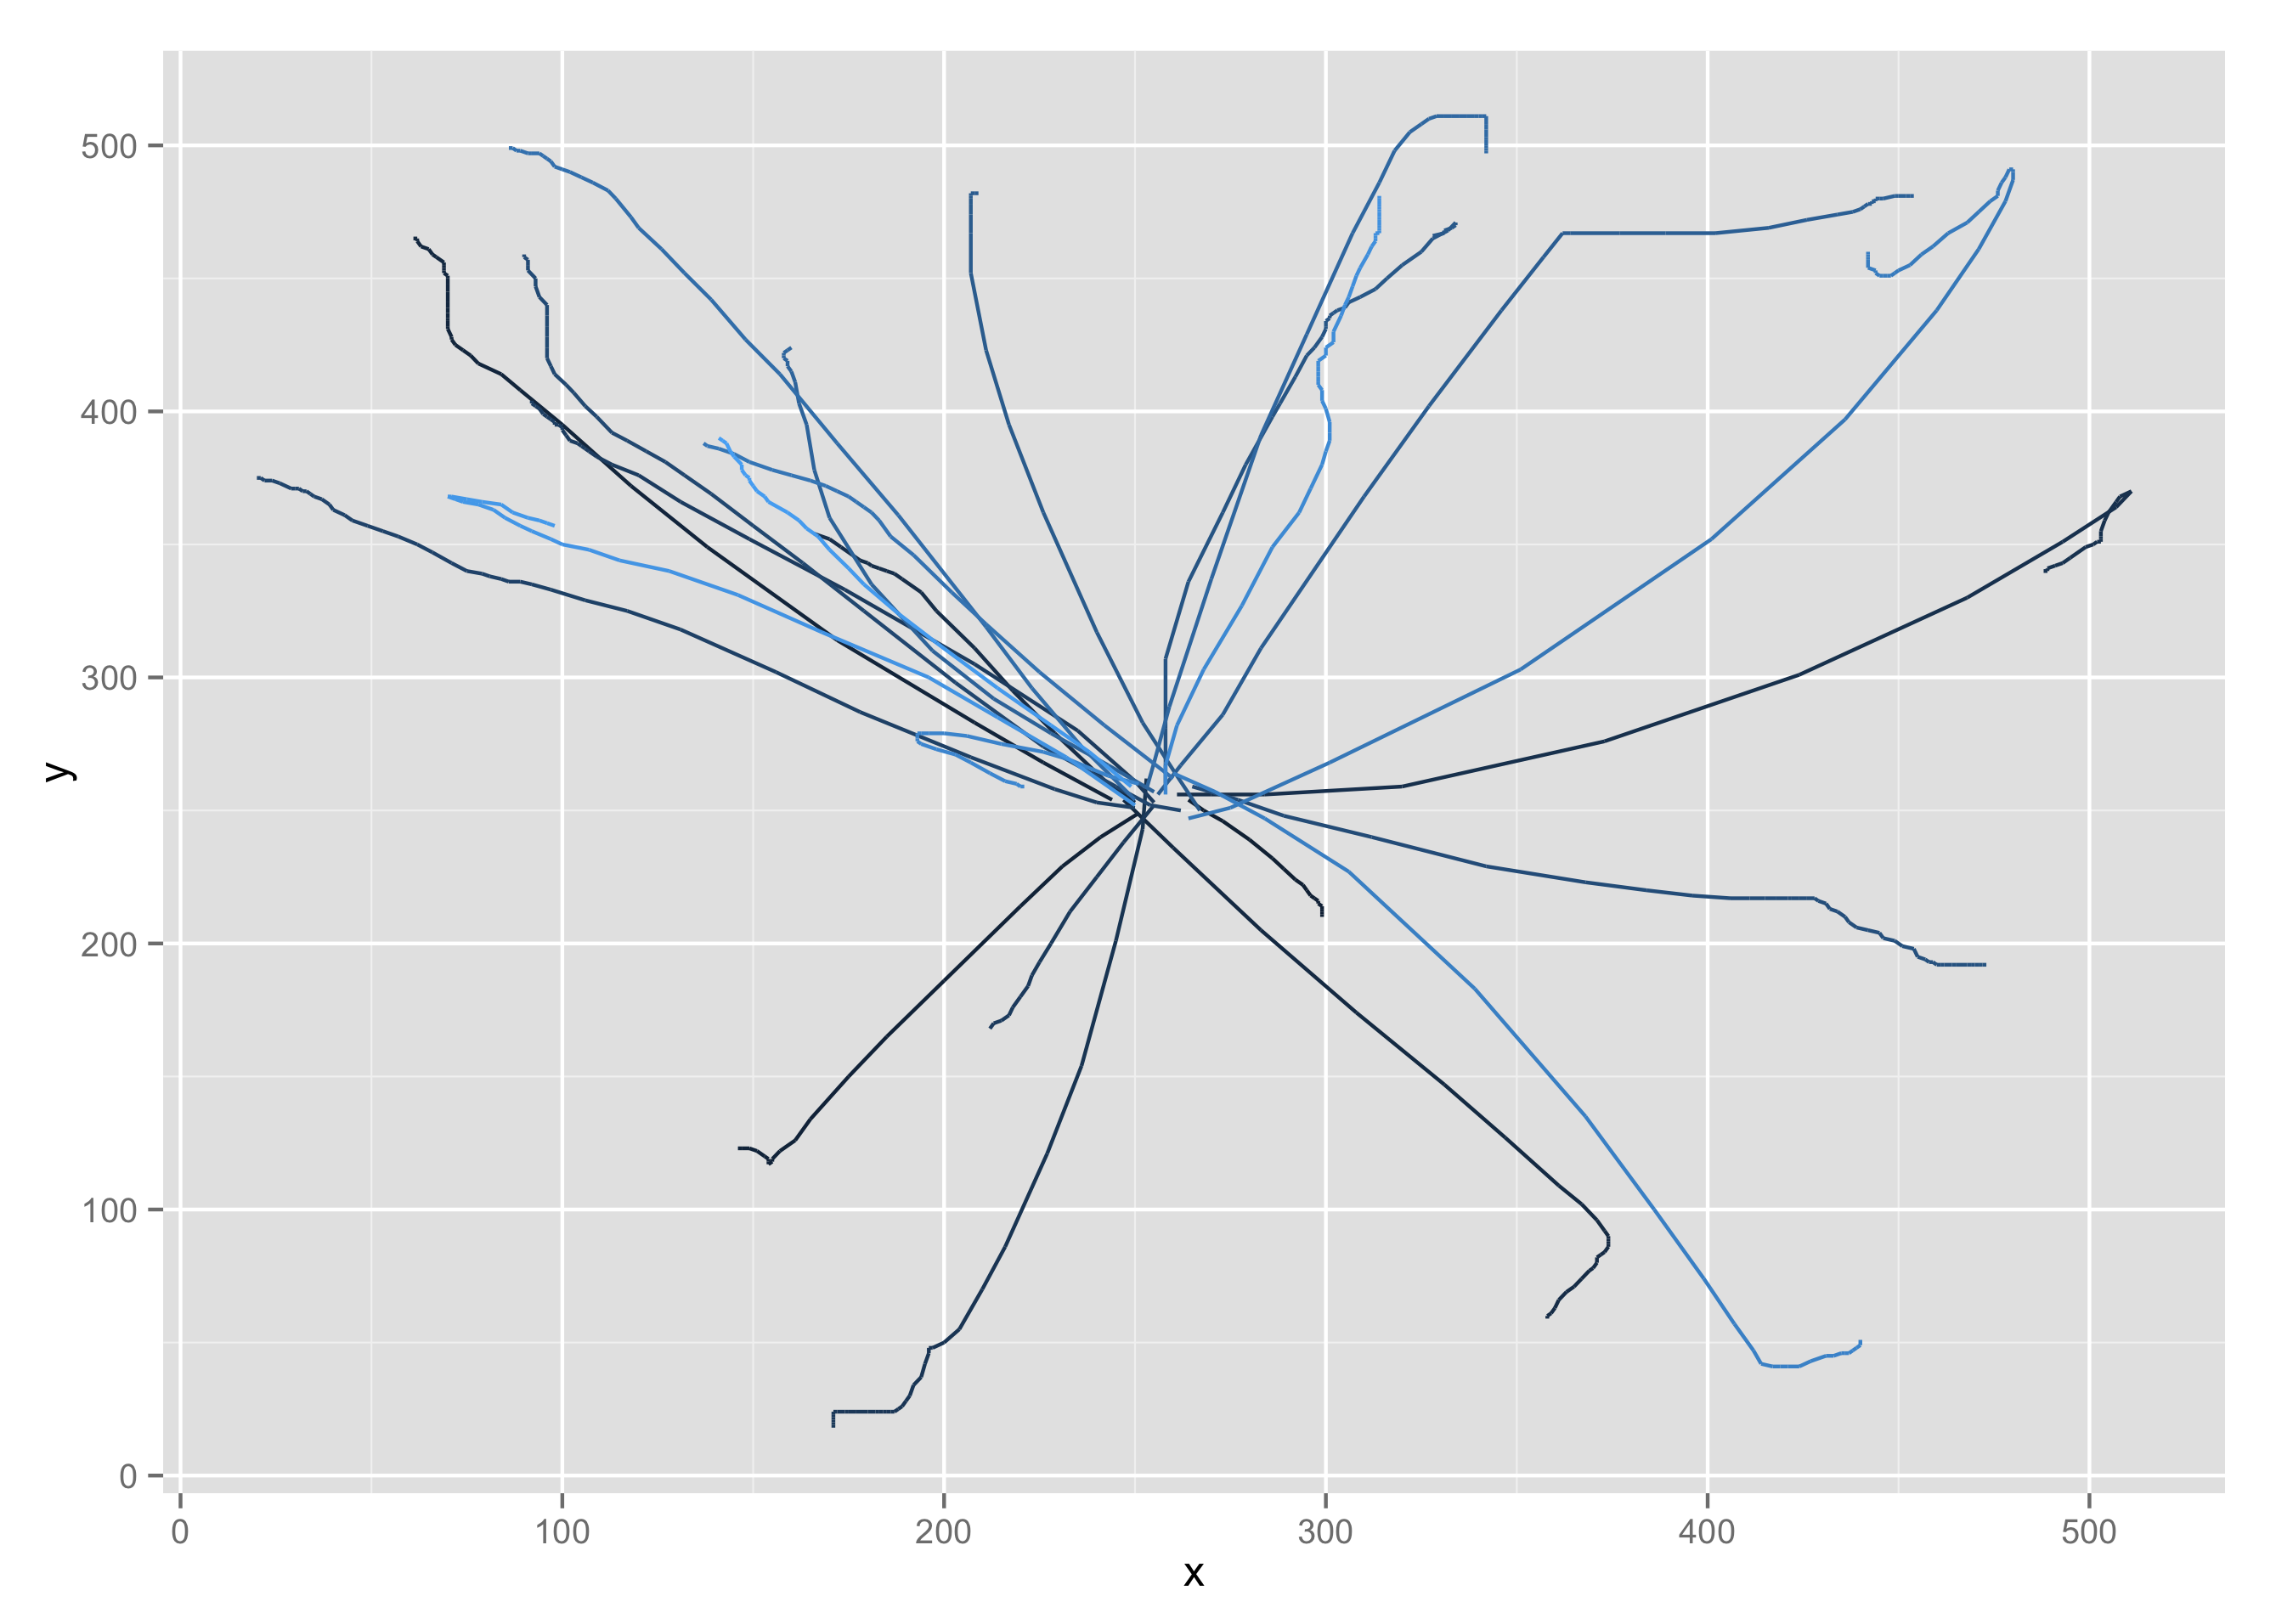
\includegraphics[width=\linewidth]{images/plots/plot_analysis_qualitative_263}
	\end{minipage}
	\begin{minipage}{0.5\linewidth}
		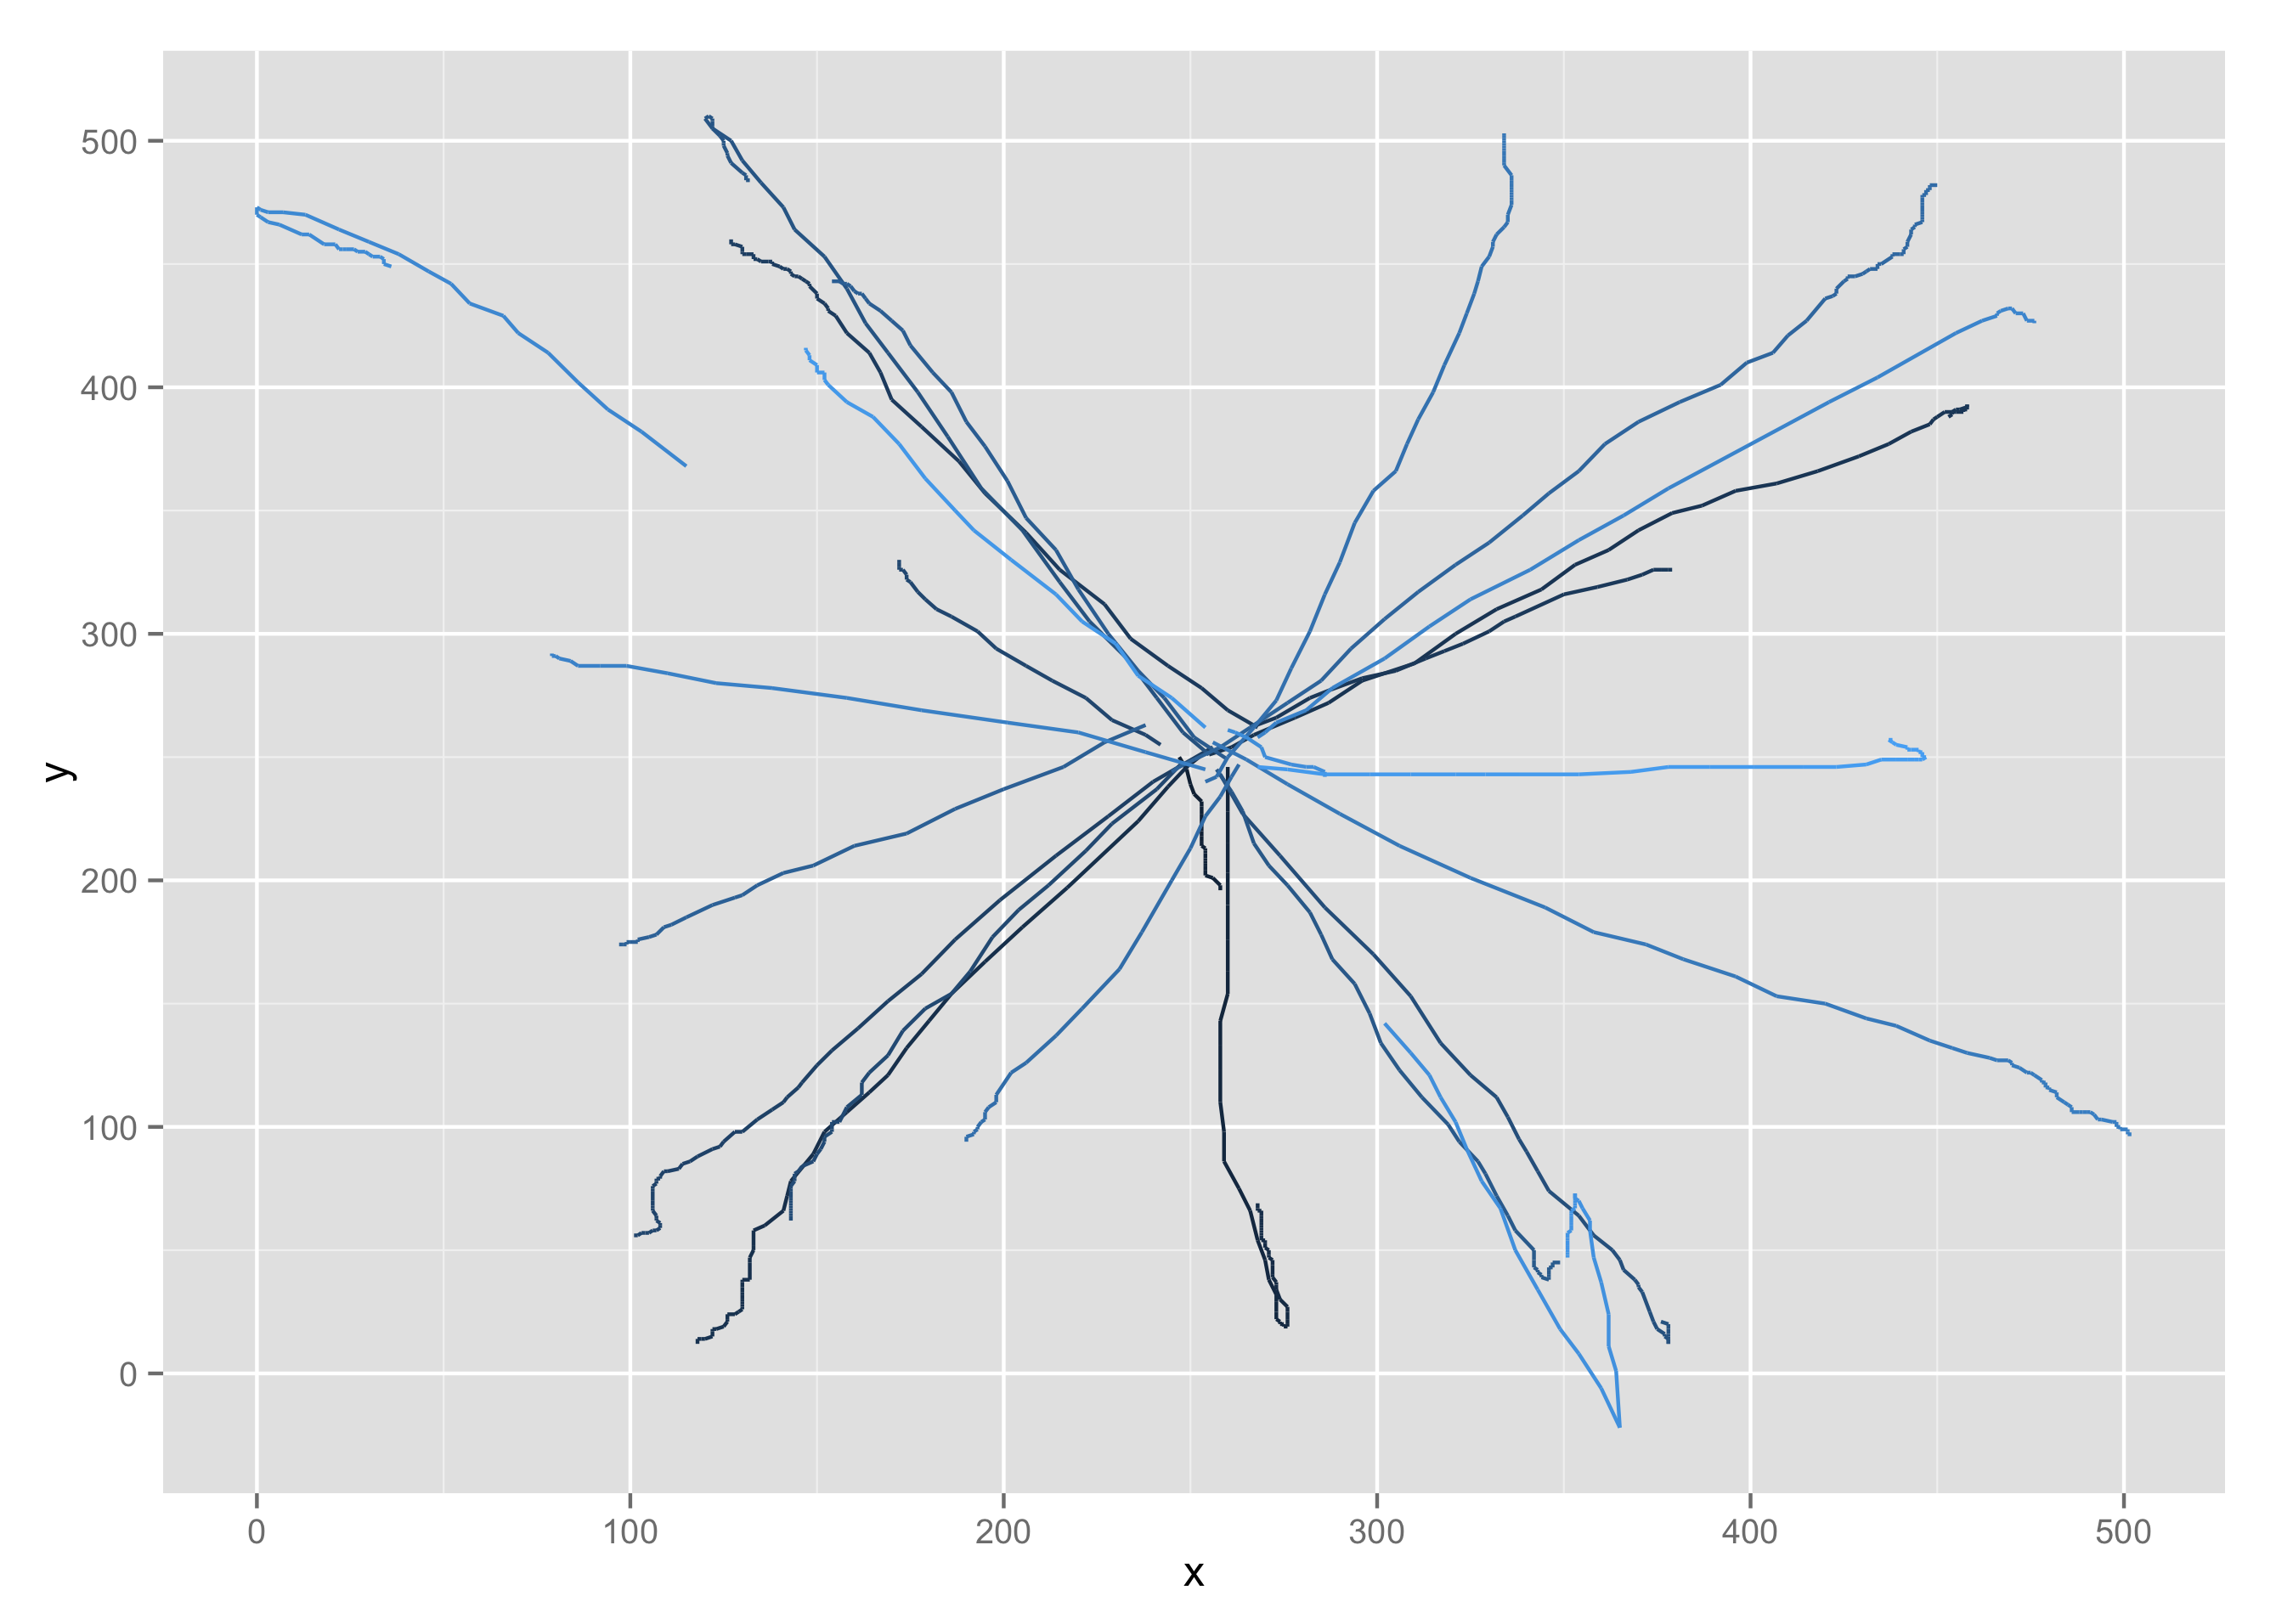
\includegraphics[width=\linewidth]{images/plots/plot_analysis_qualitative_166}
	\end{minipage}
		\begin{minipage}{0.5\linewidth}
		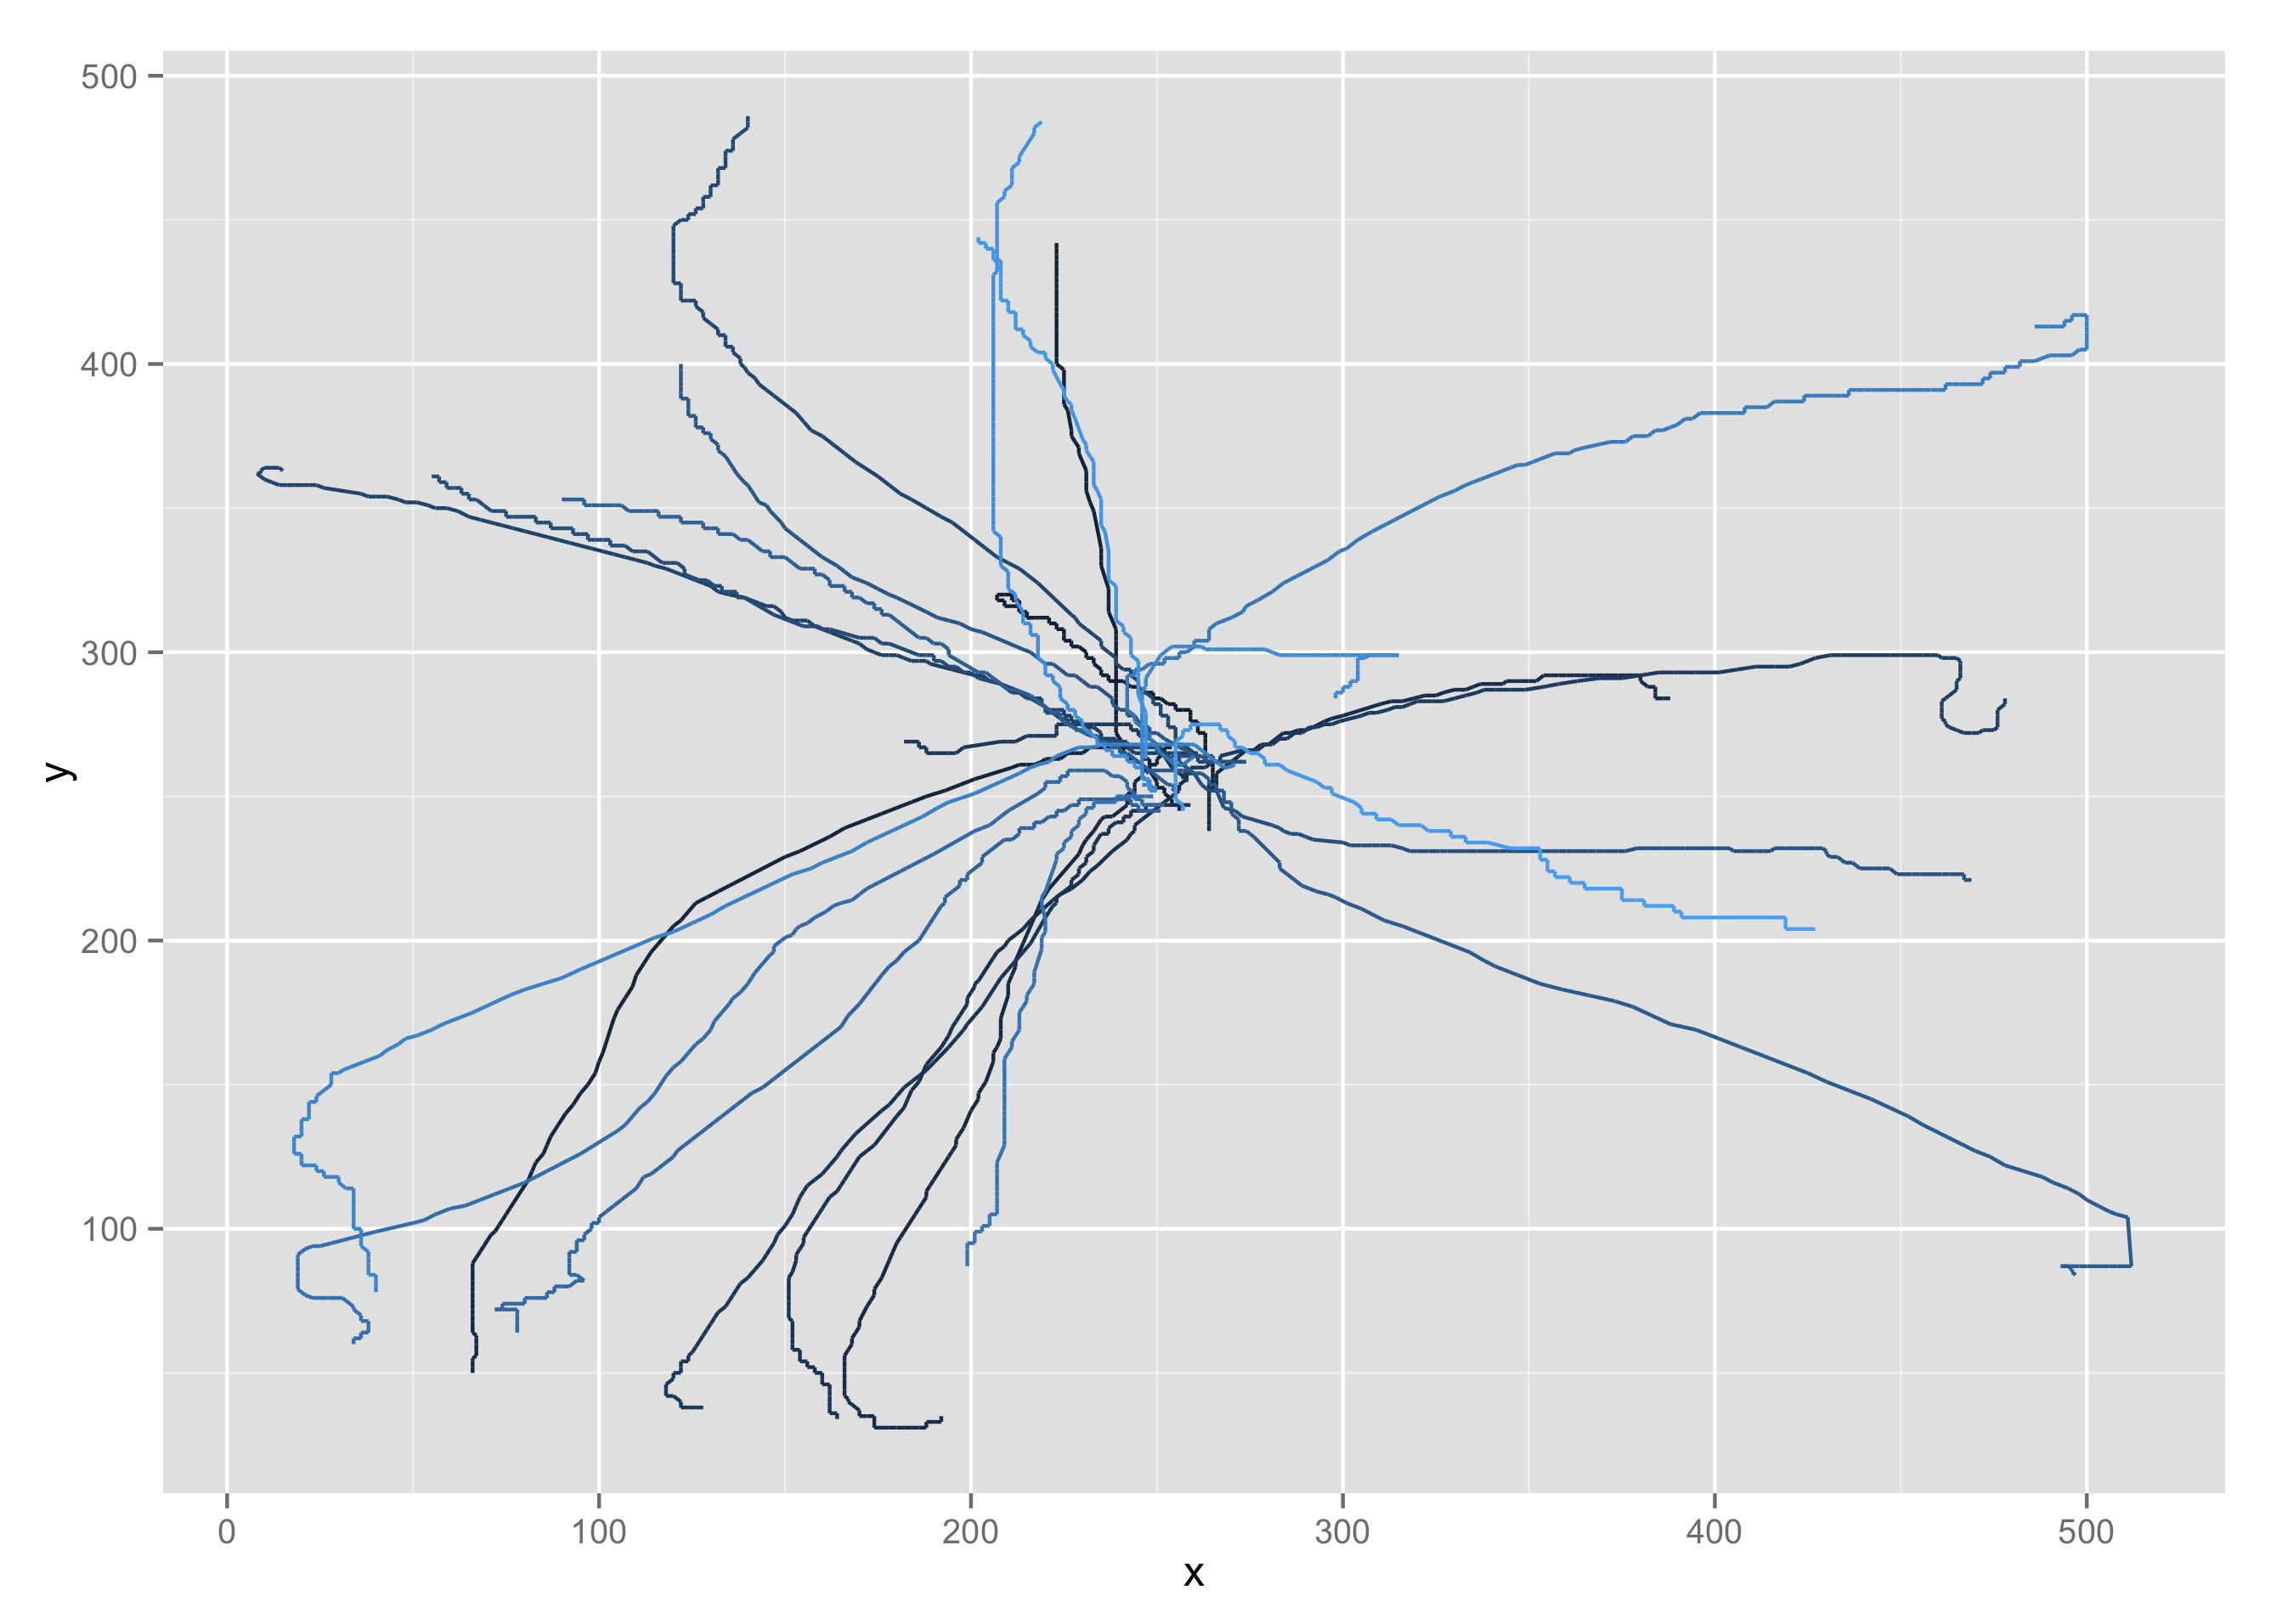
\includegraphics[width=\linewidth]{images/plots/plot_analysis_qualitative_72}
	\end{minipage}
	\begin{minipage}{0.5\linewidth}
		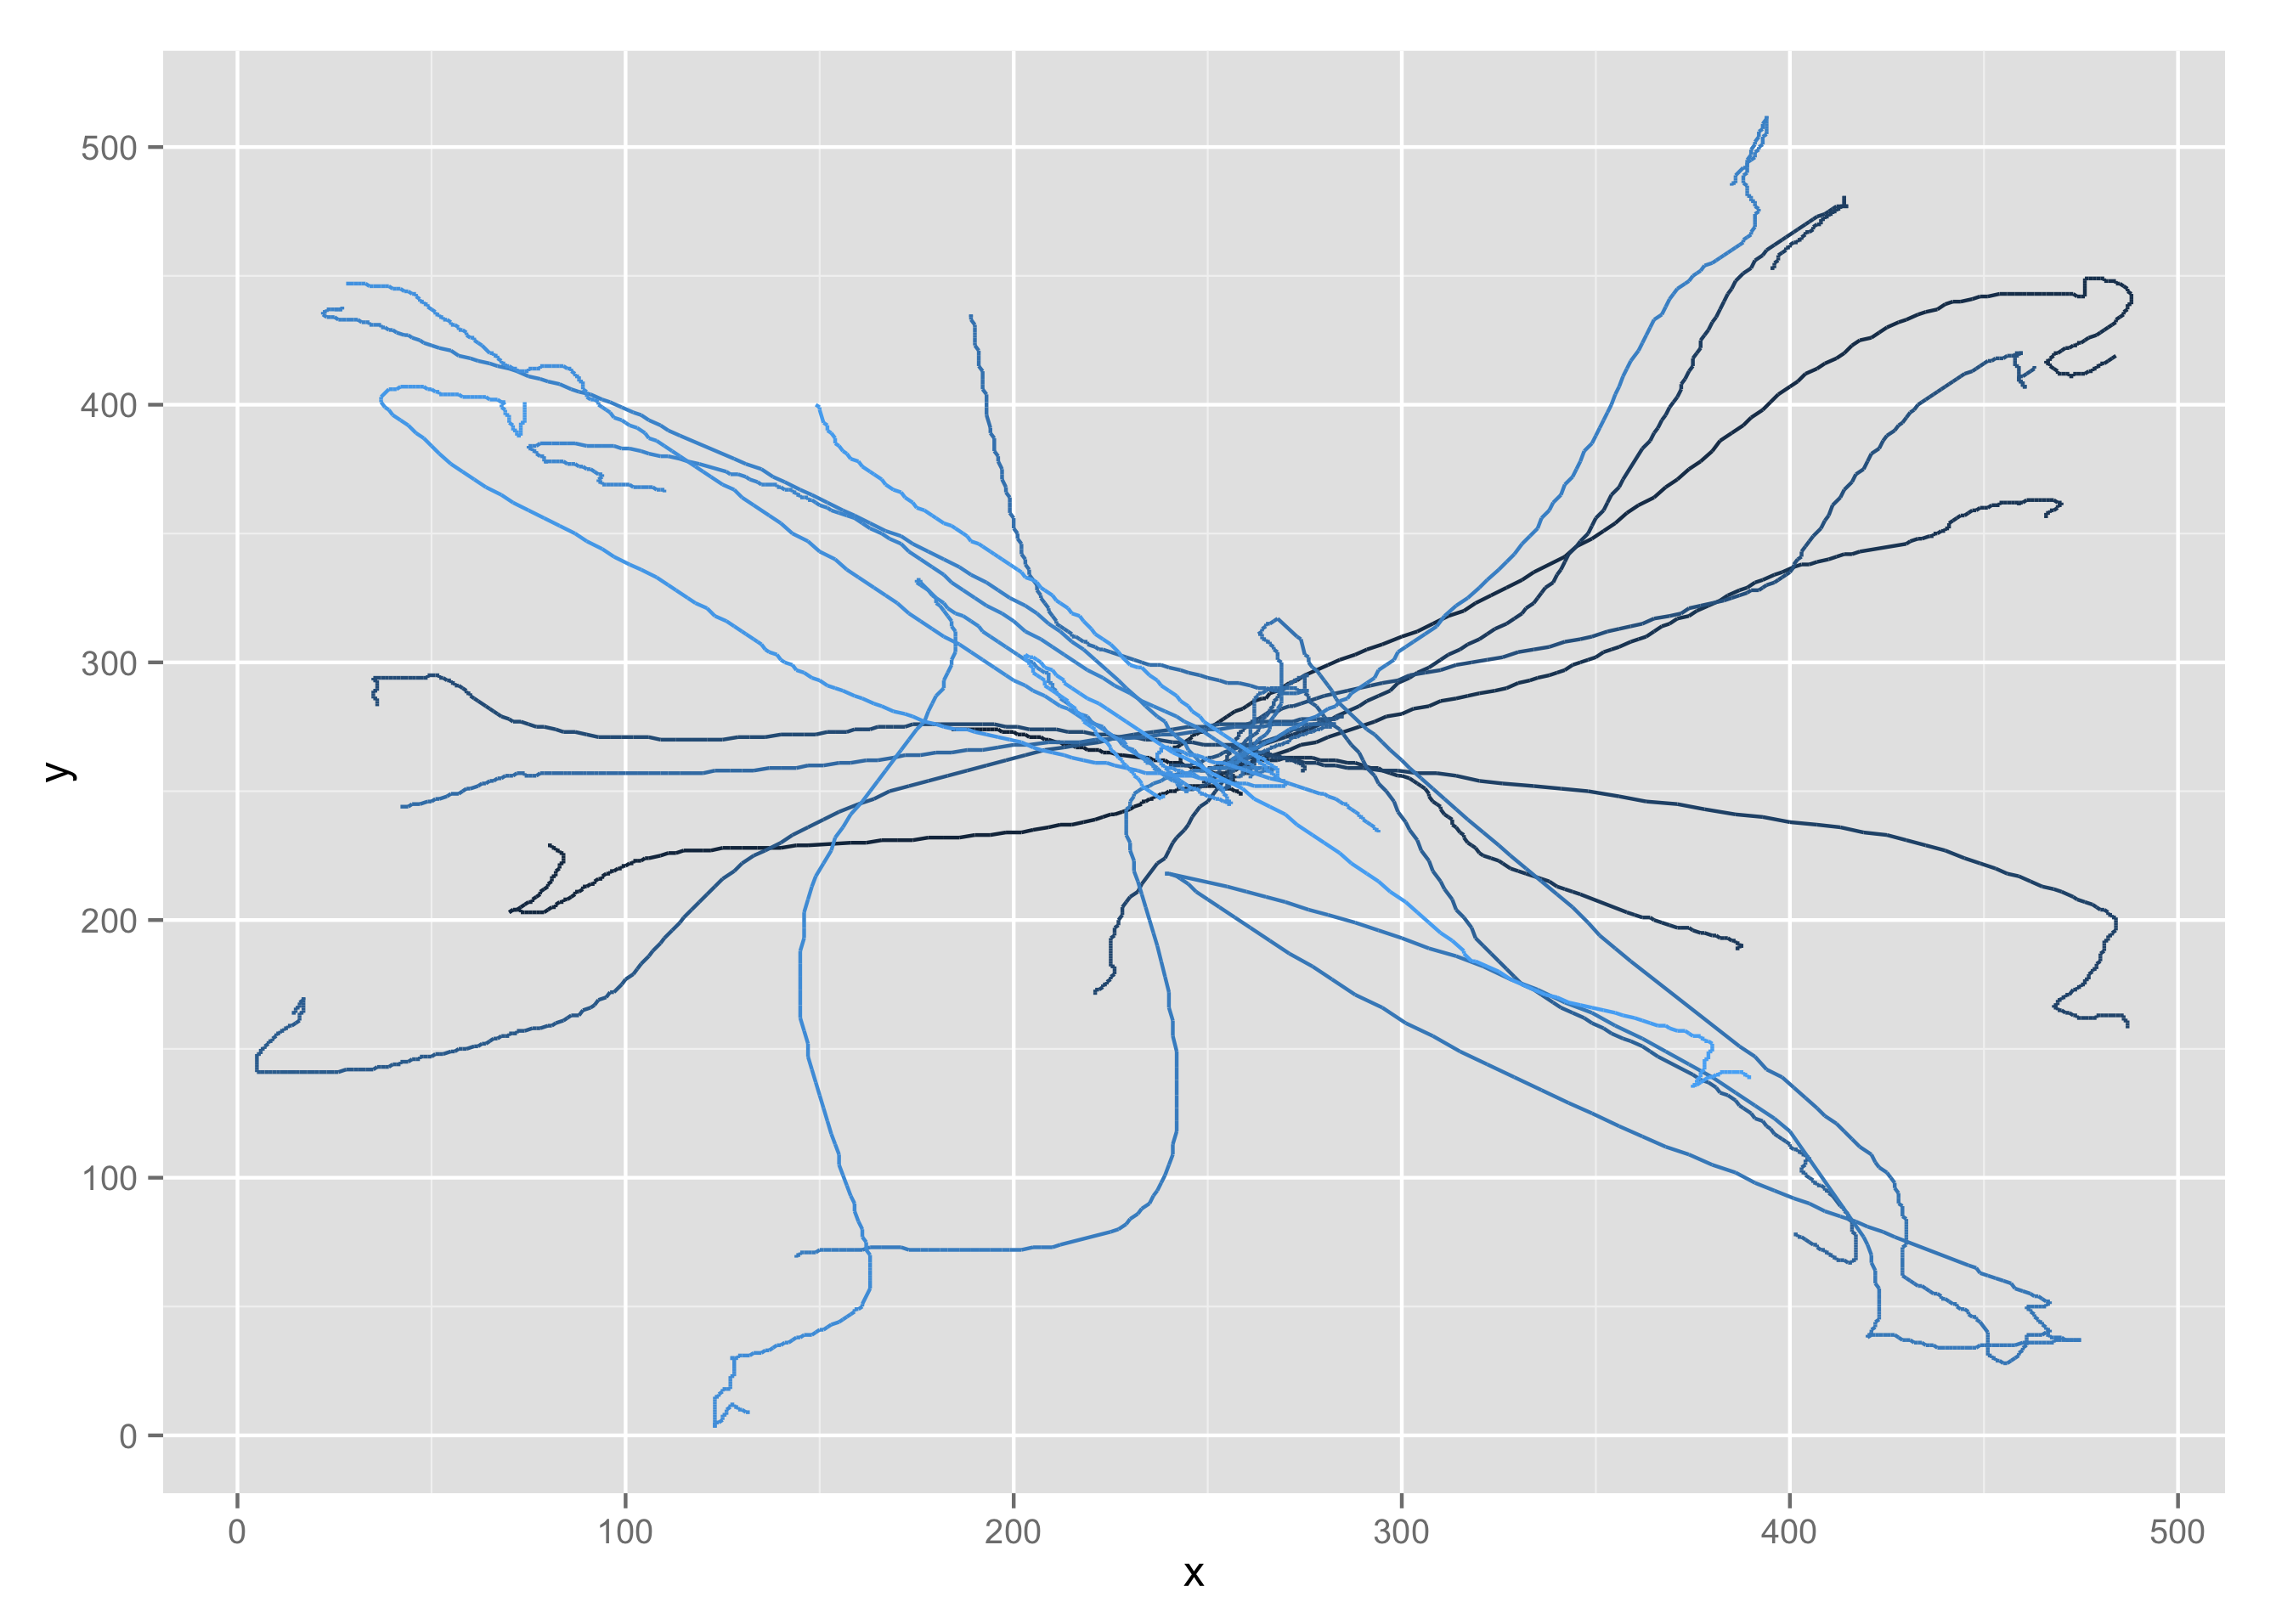
\includegraphics[width=\linewidth]{images/plots/plot_analysis_qualitative_151}
	\end{minipage}
	\begin{minipage}{0.5\linewidth}
		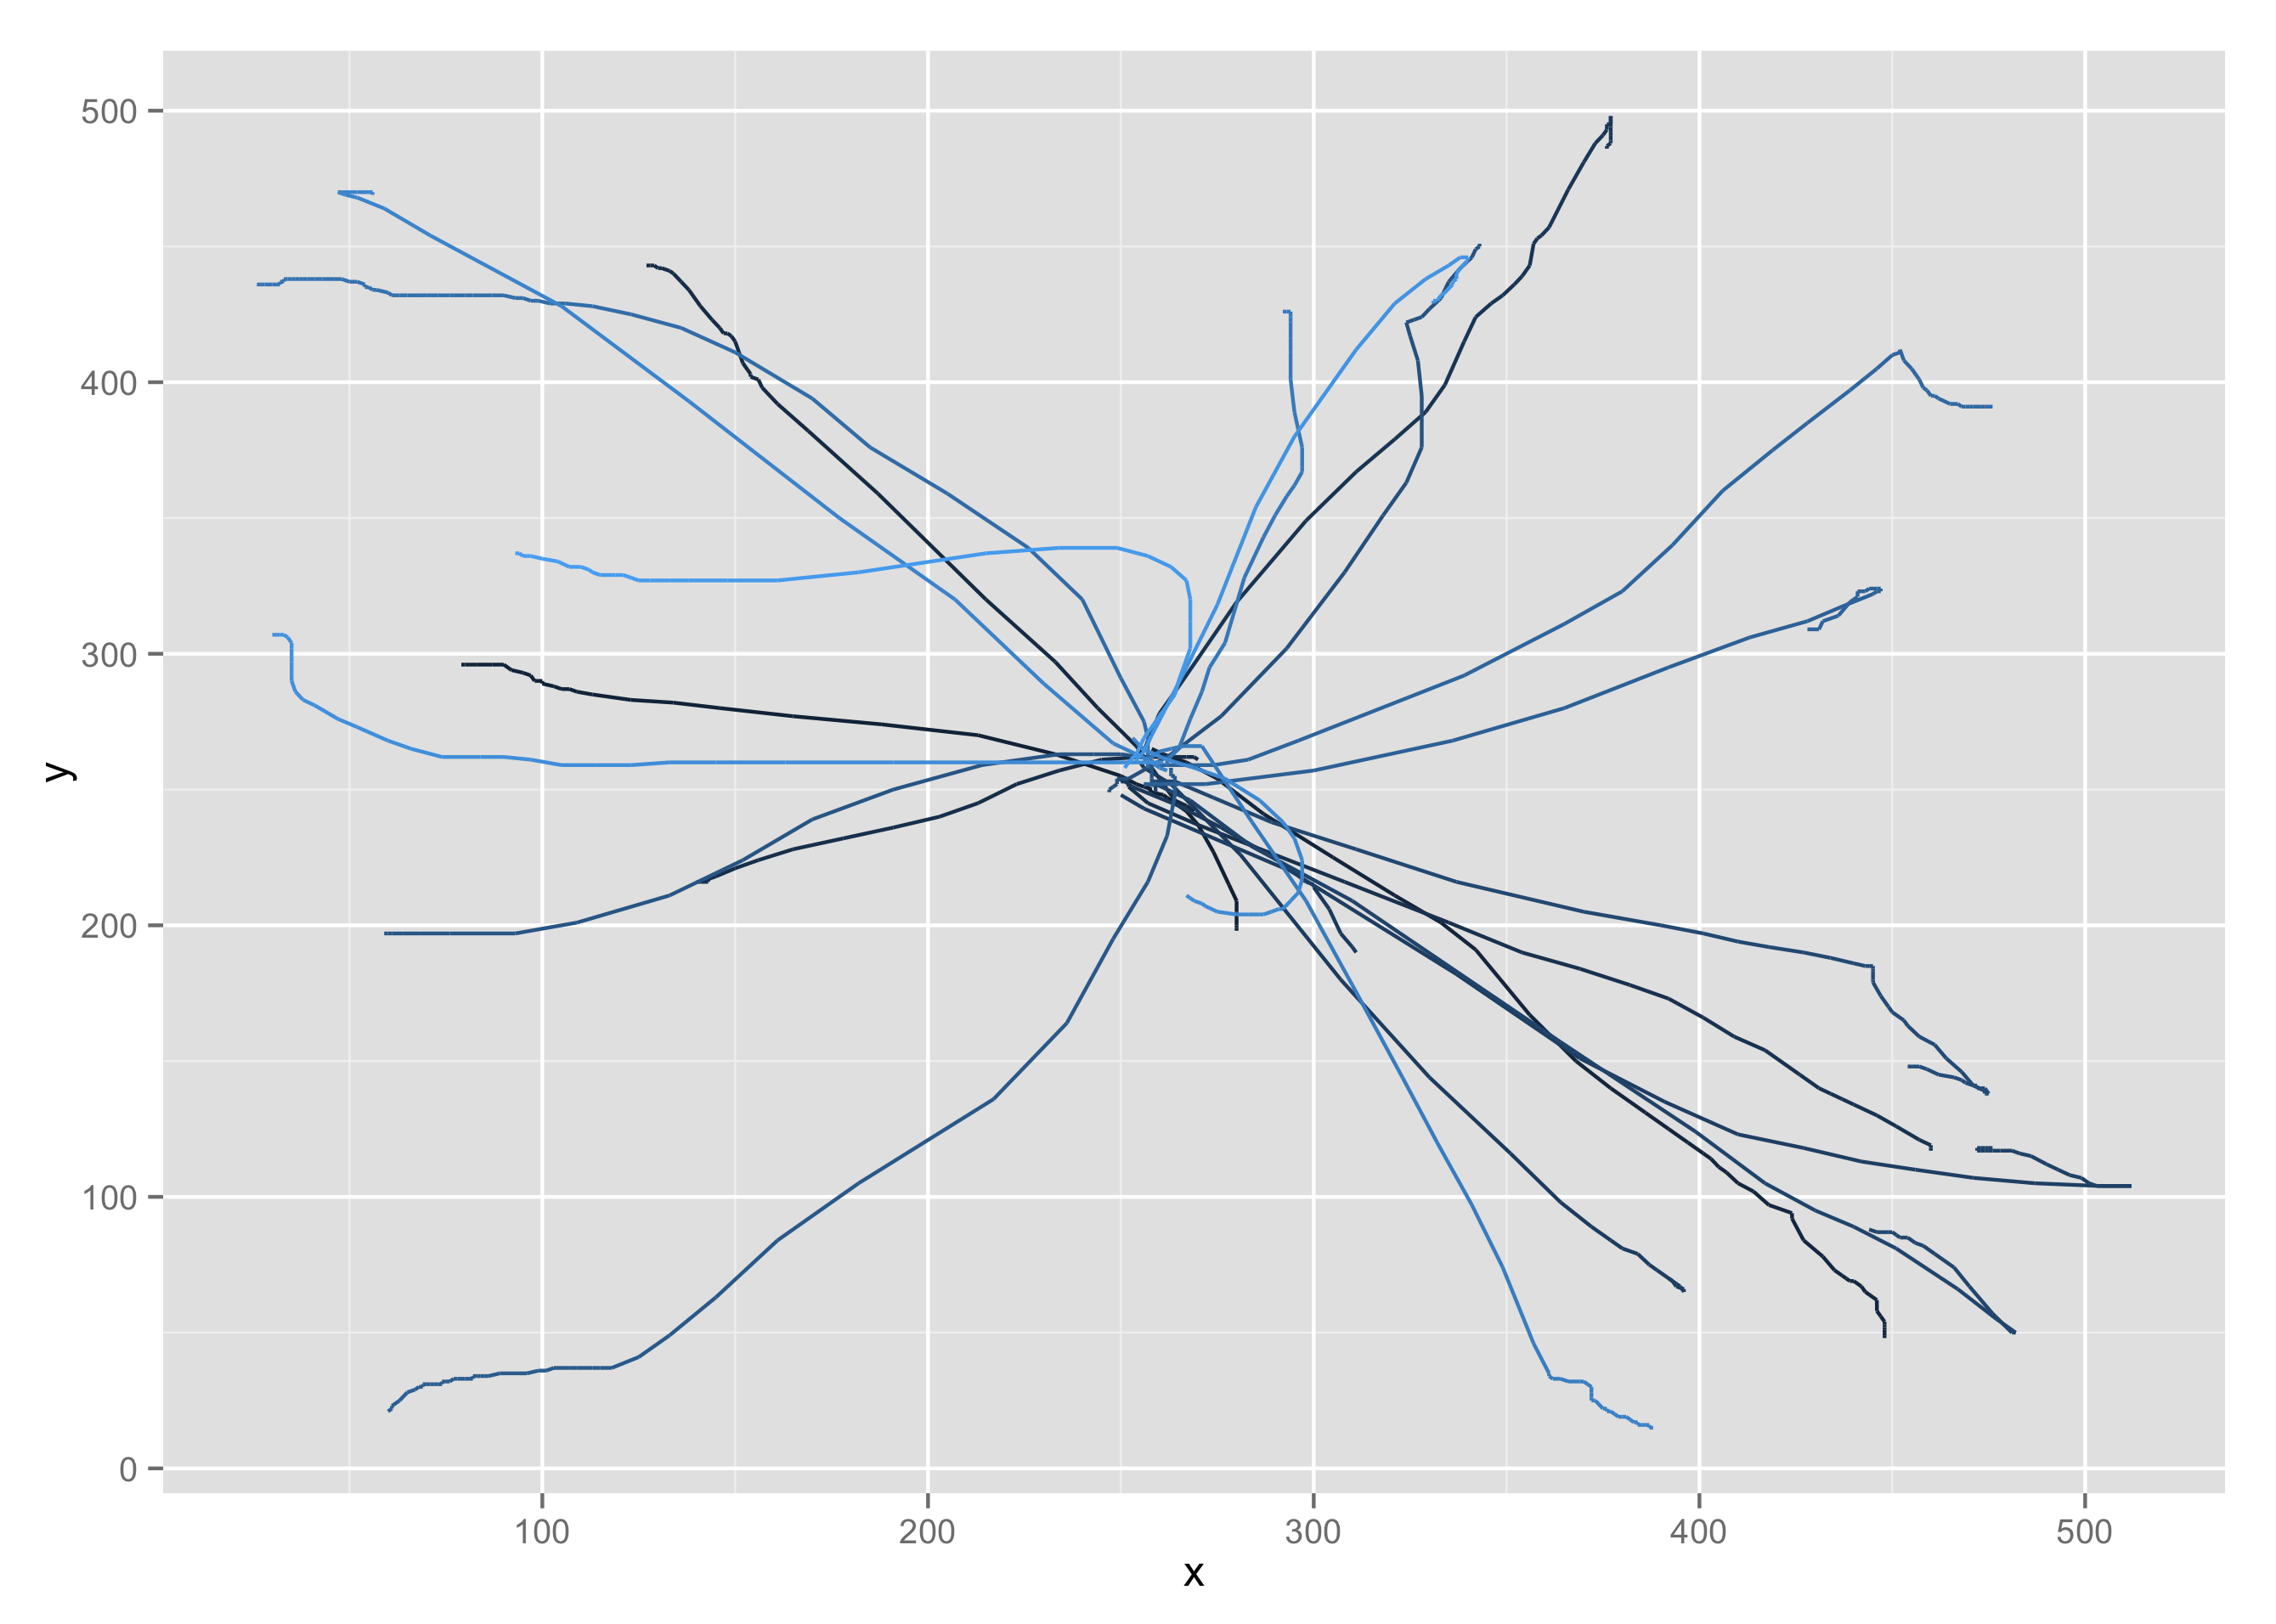
\includegraphics[width=\linewidth]{images/plots/plot_analysis_qualitative_170}
	\end{minipage}
	\begin{minipage}{0.5\linewidth}
		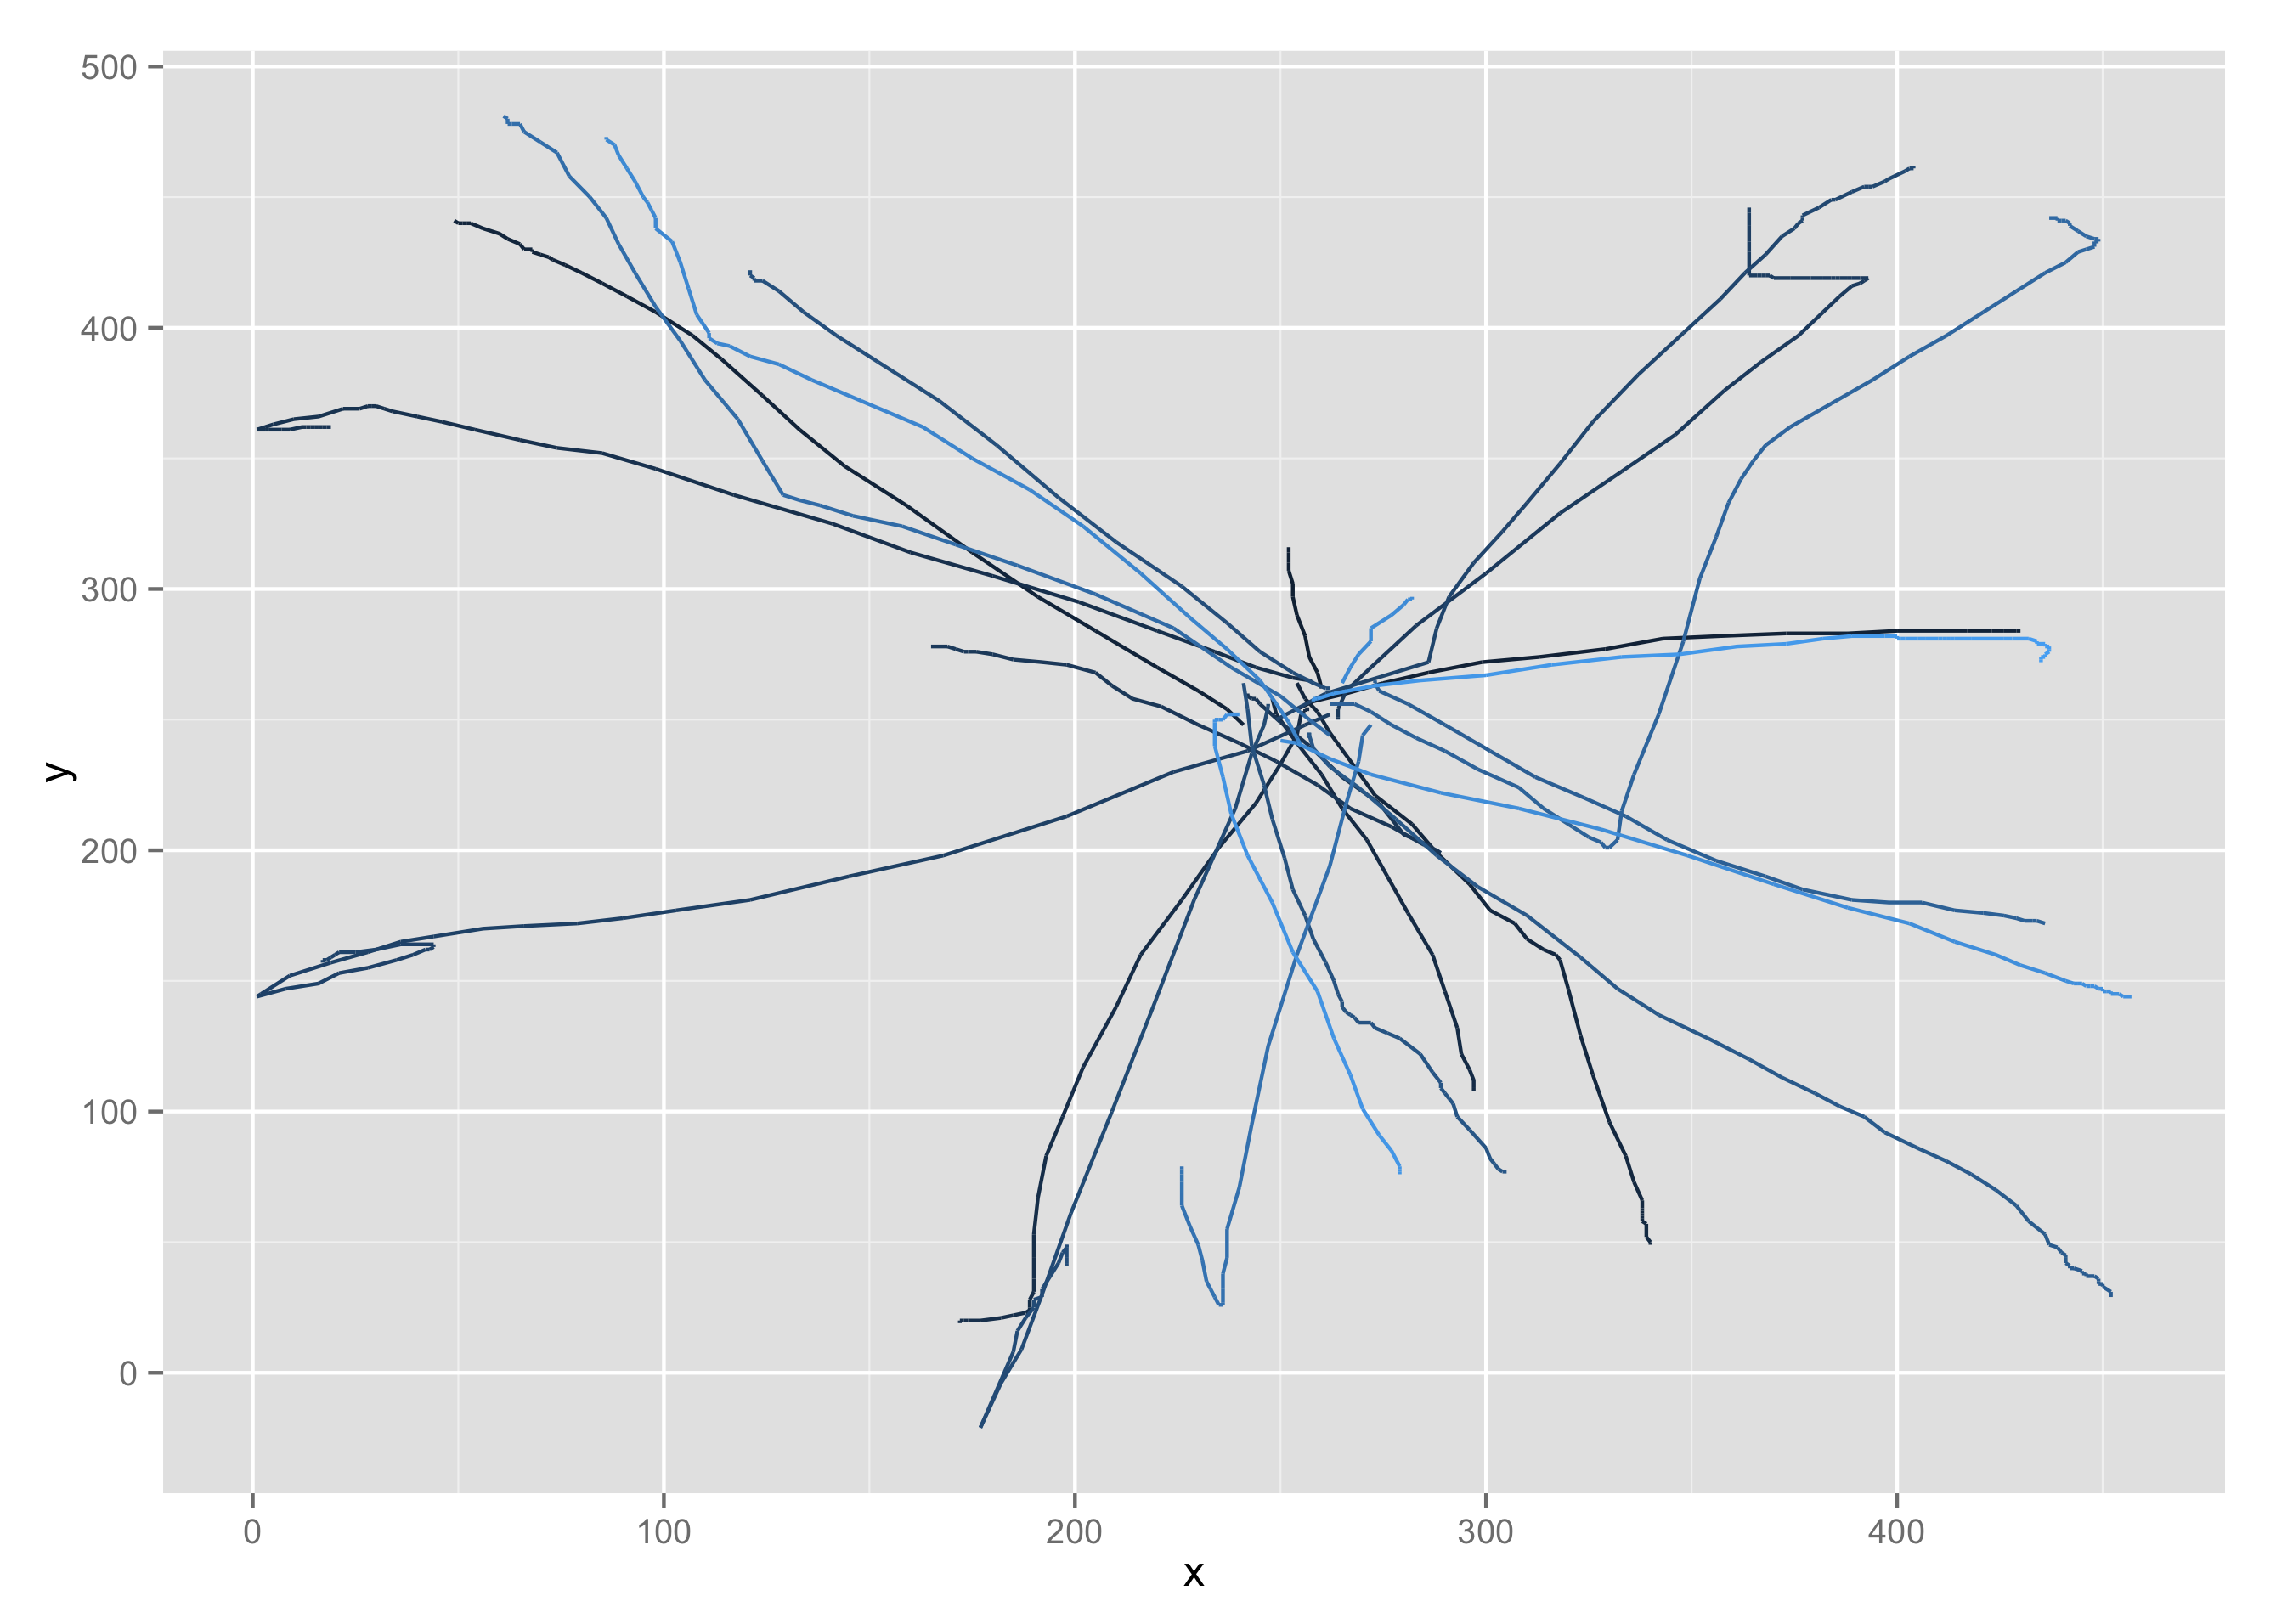
\includegraphics[width=\linewidth]{images/plots/plot_analysis_qualitative_176}
	\end{minipage}
	\begin{minipage}{0.5\linewidth}
		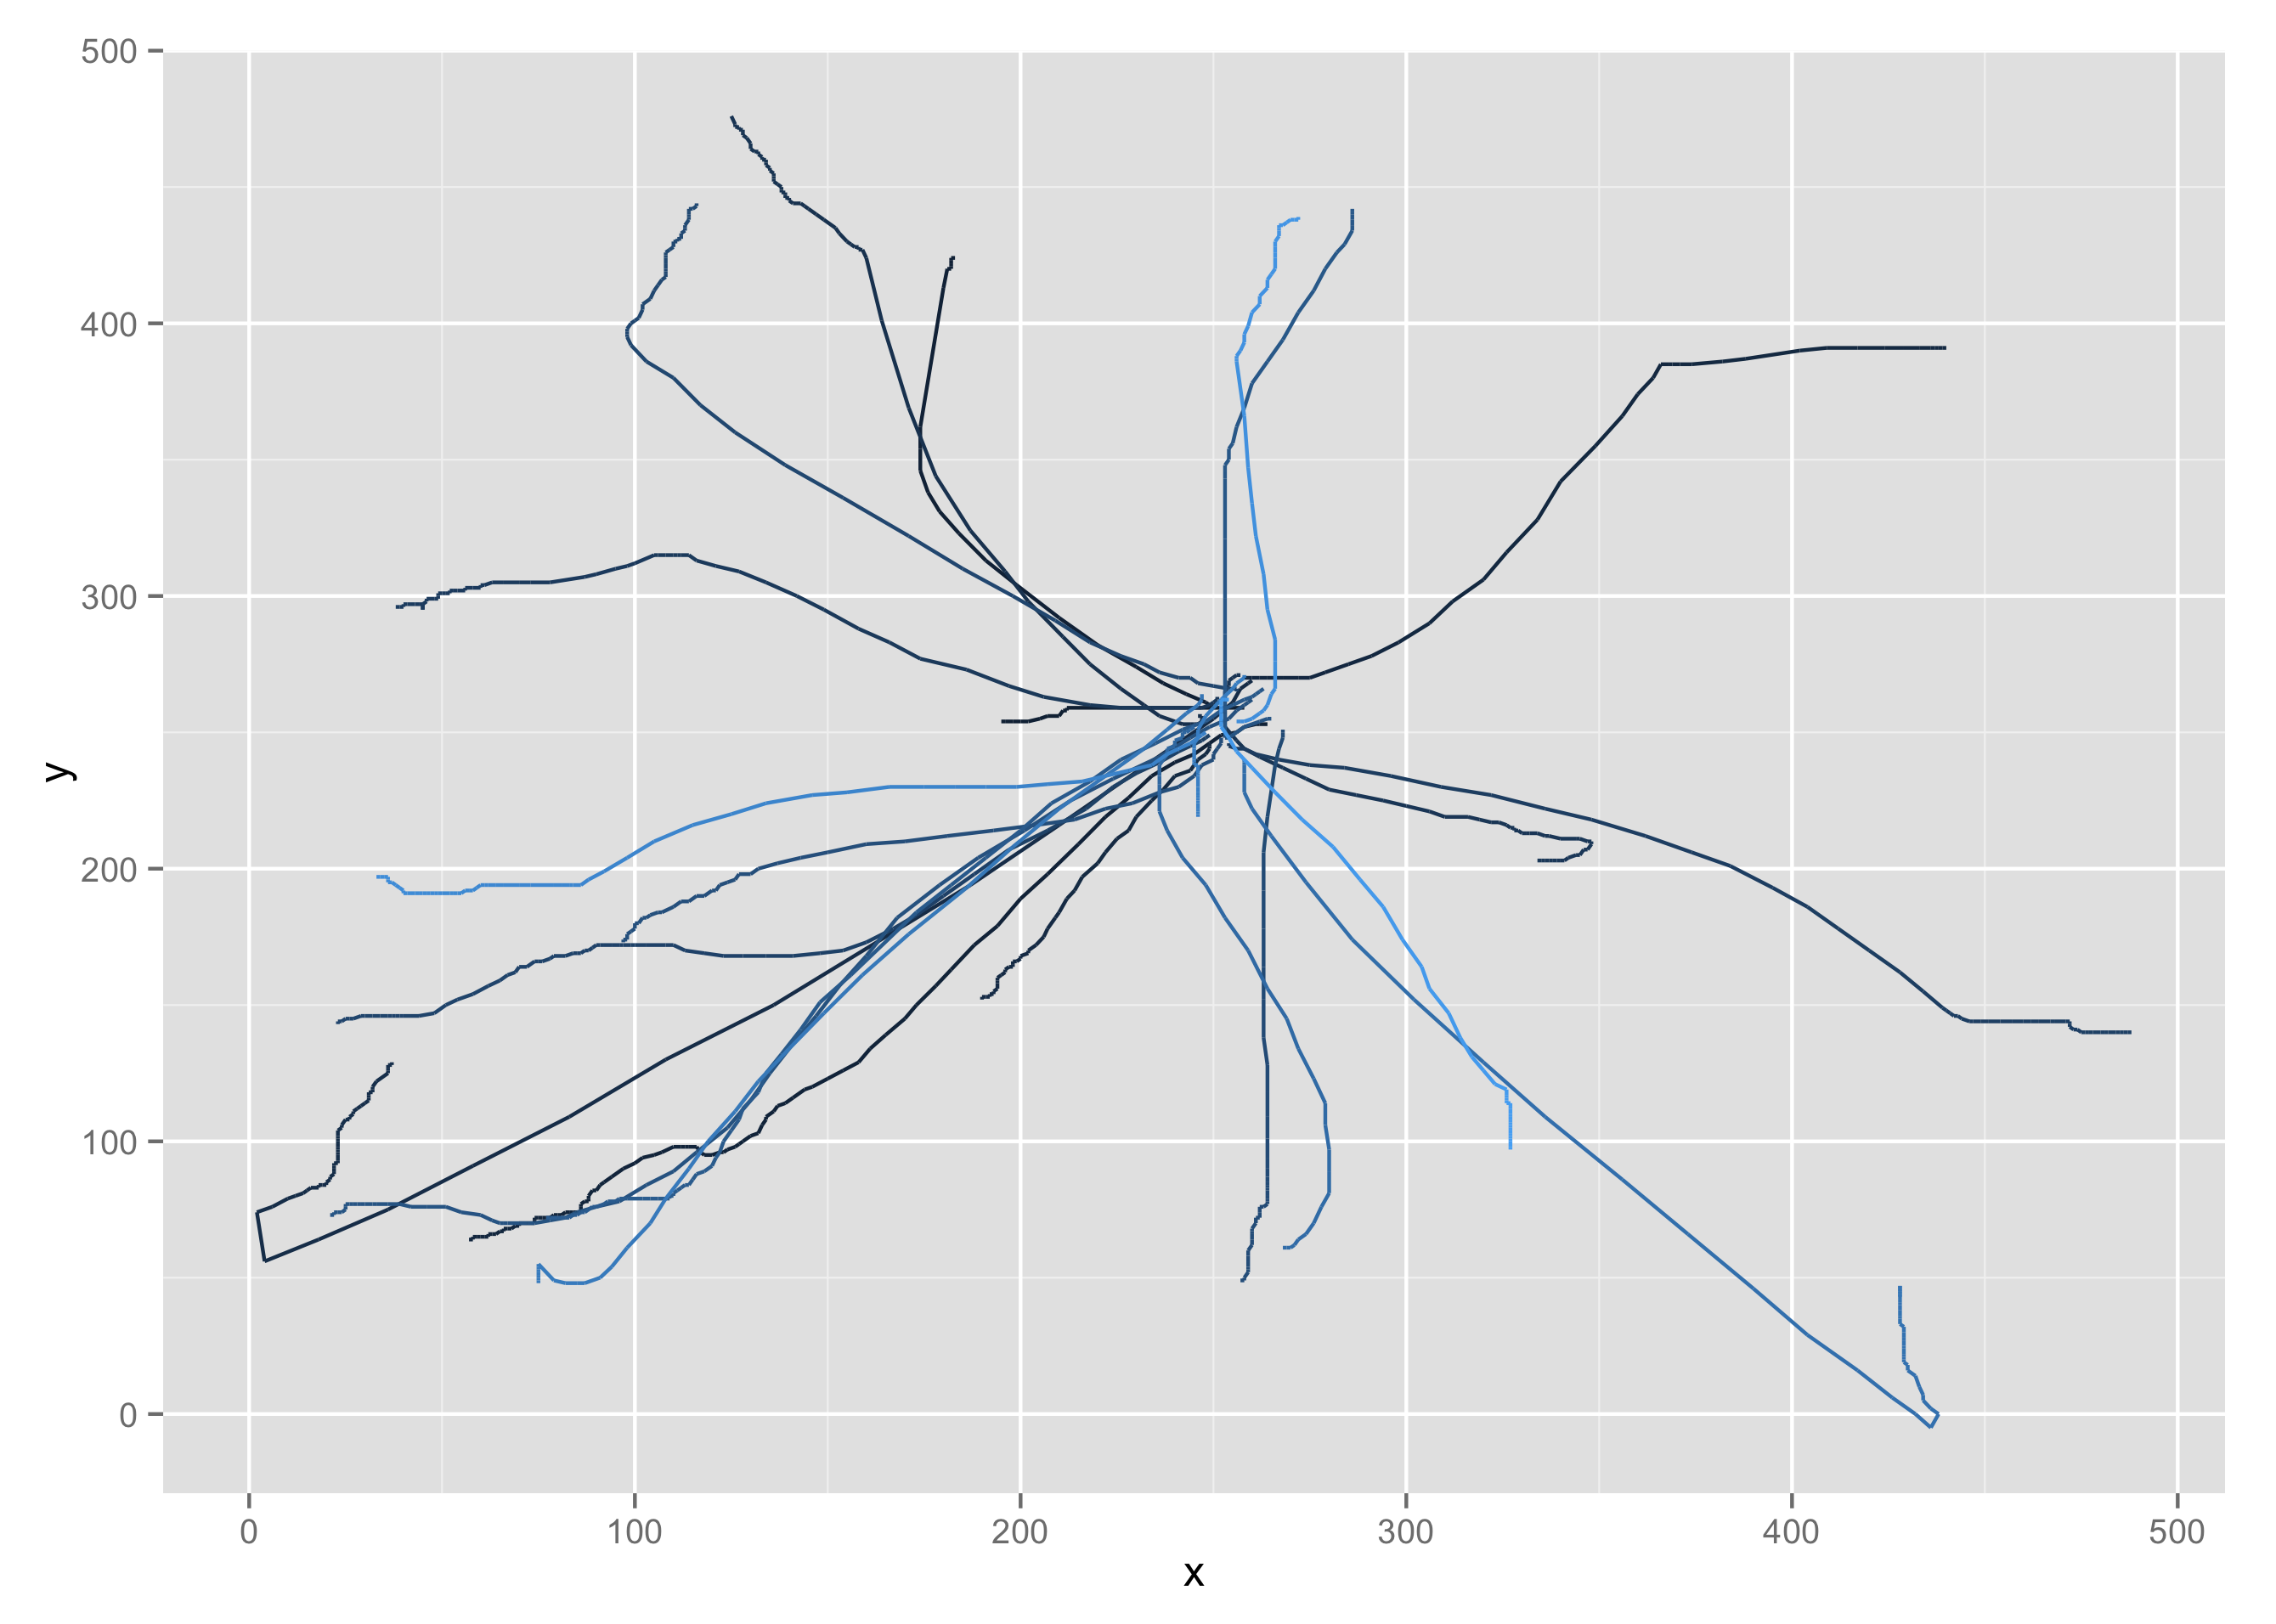
\includegraphics[width=\linewidth]{images/plots/plot_analysis_qualitative_154}
	\end{minipage}
	\captionof{figure}{8 testdeltageres bevægelsesbaner for de 25 pegeopgaver}
	\label{fig:kvaliativ_persons_2}
\end{minipage}


\begin{minipage}{\textwidth}
	\begin{minipage}{0.5\linewidth}
		\includegraphics[width=\linewidth]{images/plots/plot_analysis_qualitative_257}
	\end{minipage}
		\begin{minipage}{0.5\linewidth}
		\includegraphics[width=\linewidth]{images/plots/plot_analysis_qualitative_114}
	\end{minipage}
	\begin{minipage}{0.5\linewidth}
		\includegraphics[width=\linewidth]{images/plots/plot_analysis_qualitative_3}
	\end{minipage}
	\begin{minipage}{0.5\linewidth}
		\includegraphics[width=\linewidth]{images/plots/plot_analysis_qualitative_78}
	\end{minipage}
	\begin{minipage}{0.5\linewidth}
		\includegraphics[width=\linewidth]{images/plots/plot_analysis_qualitative_171}
	\end{minipage}
	\begin{minipage}{0.5\linewidth}
		\includegraphics[width=\linewidth]{images/plots/plot_analysis_qualitative_219}
	\end{minipage}
	\captionof{figure}{6 testdeltageres bevægelsesbaner for de 25 pegeopgaver}
	\label{fig:kvaliativ_persons_3}
\end{minipage}


%-- R-kode --%
\newpage
\chapter{R-kode fra analyse}
\label{sec:r-code}
\lstinputlisting[language=R]{main.r}

\end{appendices}
\addcontentsline{toc}{chapter}{\bibname}
\printbibliography
\end{document}
